%%%%%%%%%%%%%%%%%%%%%%%%%%%%%%%%%%%%%%%%
% datoteka diploma-vzorec.tex
%
% vzorčna datoteka za pisanje diplomskega dela v formatu LaTeX
% na UL Fakulteti za računalništvo in informatiko
%
% vkup spravil Gašper Fijavž, december 2010
% 
%
%
% verzija 12. februar 2014 (besedilo teme, seznam kratic, popravki Gašper Fijavž)
% verzija 10. marec 2014 (redakcijski popravki Zoran Bosnić)
% verzija 11. marec 2014 (redakcijski popravki Gašper Fijavž)
% verzija 15. april 2014 (pdf/a 1b compliance, not really - just claiming, Damjan Cvetan, Gašper Fijavž)
% verzija 23. april 2014 (privzeto cc licenca)
% verzija 16. september 2014 (odmiki strain od roba)
% verzija 28. oktober 2014 (odstranil vpisno številko)
% verija 5. februar 2015 (Literatura v kazalu, online literatura)
% verzija 25. september 2015 (angl. naslov v izjavi o avtorstvu)
% verzija 26. februar 2016 (UL izjava o avtorstvu)
% verzija 16. april 2016 (odstranjena izjava o avtorstvu)
% verzija 5. junij 2016 (Franc Solina dodal vrstice, ki jih je označil s svojim imenom)


\documentclass[a4paper, 12pt]{book}
%\documentclass[a4paper, 12pt, draft]{book} % Nalogo preverite tudi z opcijo draft, ki vam bo pokazala, katere vrstice so predolge!

\usepackage[utf8x]{inputenc}   % omogoča uporabo slovenskih črk kodiranih v formatu UTF-8
\usepackage[slovene,english]{babel}    % naloži, med drugim, slovenske delilne vzorce
\usepackage[pdftex]{graphicx}  % omogoča vlaganje slik različnih formatov
\usepackage{fancyhdr}          % poskrbi, na primer, za glave strani
\usepackage{amssymb}           % dodatni simboli
\usepackage{amsmath}           % eqref, npr.
%\usepackage{hyperxmp}
\usepackage[hyphens]{url}  % dodal Solina
\usepackage{comment}       % dodal Solina

\usepackage[pdftex, colorlinks=true,
						citecolor=black, filecolor=black, 
						linkcolor=black, urlcolor=black,
						pagebackref=false, 
						pdfproducer={LaTeX}, pdfcreator={LaTeX}, hidelinks]{hyperref}

\usepackage{color}       % dodal Solina
\usepackage{soul}       % dodal Solina

%%%%%%%%%%%%%%%%%%%%%%%%%%%%%%%%%%%%%%%%
%	DIPLOMA INFO
%%%%%%%%%%%%%%%%%%%%%%%%%%%%%%%%%%%%%%%%
\newcommand{\ttitle}{Učenje igranja realno-časovne strateške igre z uporabo globokega spodbujevalnega učenja}
\newcommand{\ttitleEn}{Learning to play a real-time strategy game with deep reinforcement learning}
\newcommand{\tsubject}{\ttitle}
\newcommand{\tsubjectEn}{\ttitleEn}
\newcommand{\tauthor}{Jernej Habjan}
\newcommand{\tkeywords}{AlphaZero, realno-časovna strateška igra, Unreal Engine}
\newcommand{\tkeywordsEn}{AlphaZero, real-time strategy game, Unreal Engine}


%%%%%%%%%%%%%%%%%%%%%%%%%%%%%%%%%%%%%%%%
%	HYPERREF SETUP
%%%%%%%%%%%%%%%%%%%%%%%%%%%%%%%%%%%%%%%%
\hypersetup{pdftitle={\ttitle}}
\hypersetup{pdfsubject=\ttitleEn}
\hypersetup{pdfauthor={\tauthor, jh0228@student.uni-lj.si}}
\hypersetup{pdfkeywords=\tkeywordsEn}

%%%%%%%%%%%%%%%%%%%%%%%%%%%%%%%%%%%%%%%%
% postavitev strani
%%%%%%%%%%%%%%%%%%%%%%%%%%%%%%%%%%%%%%%%  

\addtolength{\marginparwidth}{-20pt} % robovi za tisk
\addtolength{\oddsidemargin}{40pt}
\addtolength{\evensidemargin}{-40pt}

\renewcommand{\baselinestretch}{1.3} % ustrezen razmik med vrsticami
\setlength{\headheight}{15pt}        % potreben prostor na vrhu
\renewcommand{\chaptermark}[1]%
{\markboth{\MakeUppercase{\thechapter.\ #1}}{}} \renewcommand{\sectionmark}[1]%
{\markright{\MakeUppercase{\thesection.\ #1}}} \renewcommand{\headrulewidth}{0.5pt} \renewcommand{\footrulewidth}{0pt}
\fancyhf{}
\fancyhead[LE,RO]{\sl \thepage} 
%\fancyhead[LO]{\sl \rightmark} \fancyhead[RE]{\sl \leftmark}
\fancyhead[RE]{\sc \tauthor}              % dodal Solina
\fancyhead[LO]{\sc Diplomska naloga}     % dodal Solina


\newcommand{\BibTeX}{{\sc Bib}\TeX}

%%%%%%%%%%%%%%%%%%%%%%%%%%%%%%%%%%%%%%%%
% naslovi
%%%%%%%%%%%%%%%%%%%%%%%%%%%%%%%%%%%%%%%%  


\newcommand{\autfont}{\Large}
\newcommand{\titfont}{\LARGE\bf}
\newcommand{\clearemptydoublepage}{\newpage{\pagestyle{empty}\cleardoublepage}}
\setcounter{tocdepth}{1}	      % globina kazala

%%%%%%%%%%%%%%%%%%%%%%%%%%%%%%%%%%%%%%%%
% konstrukti
%%%%%%%%%%%%%%%%%%%%%%%%%%%%%%%%%%%%%%%%  
\newtheorem{izrek}{Izrek}[chapter]
\newtheorem{trditev}{Trditev}[izrek]
\newenvironment{dokaz}{\emph{Dokaz.}\ }{\hspace{\fill}{$\Box$}}

%%%%%%%%%%%%%%%%%%%%%%%%%%%%%%%%%%%%%%%%%%%%%%%%%%%%%%%%%%%%%%%%%%%%%%%%%%%%%%%
%% PDF-A
%%%%%%%%%%%%%%%%%%%%%%%%%%%%%%%%%%%%%%%%%%%%%%%%%%%%%%%%%%%%%%%%%%%%%%%%%%%%%%%


%%%%%%%%%%%%%%%%%%%%%%%%%%%%%%%%%%%%%%%% 
% define medatata
%%%%%%%%%%%%%%%%%%%%%%%%%%%%%%%%%%%%%%%% 
\def\Title{\ttitle}
\def\Author{\tauthor, jh0228@student.uni-lj.si}
\def\Subject{\ttitleEn}
\def\Keywords{\tkeywordsEn}

%%%%%%%%%%%%%%%%%%%%%%%%%%%%%%%%%%%%%%%% 
% \convertDate converts D:20080419103507+02'00' to 2008-04-19T10:35:07+02:00
%%%%%%%%%%%%%%%%%%%%%%%%%%%%%%%%%%%%%%%% 
\def\convertDate{%
    \getYear
}

{\catcode`\D=12
 \gdef\getYear D:#1#2#3#4{\edef\xYear{#1#2#3#4}\getMonth}
}
\def\getMonth#1#2{\edef\xMonth{#1#2}\getDay}
\def\getDay#1#2{\edef\xDay{#1#2}\getHour}
\def\getHour#1#2{\edef\xHour{#1#2}\getMin}
\def\getMin#1#2{\edef\xMin{#1#2}\getSec}
\def\getSec#1#2{\edef\xSec{#1#2}\getTZh}
\def\getTZh +#1#2{\edef\xTZh{#1#2}\getTZm}
\def\getTZm '#1#2'{%
    \edef\xTZm{#1#2}%
    \edef\convDate{\xYear-\xMonth-\xDay T\xHour:\xMin:\xSec+\xTZh:\xTZm}%
}

\expandafter\convertDate\pdfcreationdate 

%%%%%%%%%%%%%%%%%%%%%%%%%%%%%%%%%%%%%%%%
% get pdftex version string
%%%%%%%%%%%%%%%%%%%%%%%%%%%%%%%%%%%%%%%% 
\newcount\countA
\countA=\pdftexversion
\advance \countA by -100
\def\pdftexVersionStr{pdfTeX-1.\the\countA.\pdftexrevision}


%%%%%%%%%%%%%%%%%%%%%%%%%%%%%%%%%%%%%%%%
% XMP data
%%%%%%%%%%%%%%%%%%%%%%%%%%%%%%%%%%%%%%%%  
\usepackage{xmpincl}
\includexmp{pdfa-1b}

%%%%%%%%%%%%%%%%%%%%%%%%%%%%%%%%%%%%%%%%
% pdfInfo
%%%%%%%%%%%%%%%%%%%%%%%%%%%%%%%%%%%%%%%%  
\pdfinfo{%
    /Title    (\ttitle)
    /Author   (\tauthor, damjan@cvetan.si)
    /Subject  (\ttitleEn)
    /Keywords (\tkeywordsEn)
    /ModDate  (\pdfcreationdate)
    /Trapped  /False
}

\usepackage{amssymb}
\usepackage{color,soulutf8}

\begin{document}
\selectlanguage{slovene}
\frontmatter
\setcounter{page}{1} %
\renewcommand{\thepage}{}       % preprecimo težave s številkami strani v kazalu
\newcommand{\sn}[1]{"`#1"'}                    % dodal Solina (slovenski narekovaji)

%%%%%%%%%%%%%%%%%%%%%%%%%%%%%%%%%%%%%%%%
%naslovnica
 \thispagestyle{empty}%
   \begin{center}
    {\large\sc Univerza v Ljubljani\\%
      Fakulteta za računalništvo in informatiko}%
    \vskip 10em%
    {\autfont \tauthor\par}%
    {\titfont \ttitle \par}%
    {\vskip 3em \textsc{DIPLOMSKO DELO\\[5mm]         % dodal Solina za ostale študijske programe
 VISOKOŠOLSKI STROKOVNI ŠTUDIJSKI PROGRAM\\ PRVE STOPNJE\\ RAČUNALNIŠTVO IN INFORMATIKA}\par}%
%    UNIVERZITETNI  ŠTUDIJSKI PROGRAM\\ PRVE STOPNJE\\ RAČUNALNIŠTVO IN INFORMATIKA}\par}%
%    INTERDISCIPLINARNI UNIVERZITETNI\\ ŠTUDIJSKI PROGRAM PRVE STOPNJE\\ RAČUNALNIŠTVO IN MATEMATIKA}\par}%
%    INTERDISCIPLINARNI UNIVERZITETNI\\ ŠTUDIJSKI PROGRAM PRVE STOPNJE\\ UPRAVNA INFORMATIKA}\par}%
%    INTERDISCIPLINARNI UNIVERZITETNI\\ ŠTUDIJSKI PROGRAM PRVE STOPNJE\\ MULTIMEDIJA}\par}%
    \vfill\null%
    {\large \textsc{Mentor}: doc.\ dr. Matej Guid\par}%
   {\large \textsc{Somentor}:  prof.\ dr. Branko Šter \par}%
    {\vskip 2em \large Ljubljana, 2019 \par}%
\end{center}
% prazna stran
%\clearemptydoublepage      % dodal Solina (izjava o licencah itd. se izpiše na hrbtni strani naslovnice)

%%%%%%%%%%%%%%%%%%%%%%%%%%%%%%%%%%%%%%%%
%copyright stran
\thispagestyle{empty}
\vspace*{8cm}

\noindent
{\sc Copyright}. 
Rezultati diplomske naloge so intelektualna lastnina avtorja in Fakultete za računalništvo in informatiko Univerze v Ljubljani.
Za objavo in koriščenje rezultatov diplomske naloge je potrebno pisno privoljenje avtorja, Fakultete za računalništvo in informatiko ter mentorja.

\begin{center}
\mbox{}\vfill
\emph{Besedilo je oblikovano z urejevalnikom besedil \LaTeX.}
\end{center}
% prazna stran
\clearemptydoublepage

%%%%%%%%%%%%%%%%%%%%%%%%%%%%%%%%%%%%%%%%
% stran 3 med uvodnimi listi
\thispagestyle{empty}
\vspace*{4cm}

\noindent
Fakulteta za računalništvo in informatiko izdaja naslednjo nalogo:
\medskip
\begin{tabbing}
\hspace{32mm}\= \hspace{6cm} \= \kill
Tematika naloge:
\end{tabbing}
Implementirajte računalniški program, ki bo kombiniral drevesno preiskovanje Monte Carlo (MCTS) in strojno učenje z globokimi nevronskimi mrežami, za inteligentno igranje realno-časovne strateške igre. Pri tem se zgledujte po algoritmu AlphaZero. Eksperimentalno ovrednotite različne konfiguracije učnih parametrov pri strojnem učenju. Kakovost igranja preverite na poljubni realno-časovni strateški igri. Uspešnost uporabljenega pristopa demonstrirajte s pomočjo grafičnega vmesnika, ki bo omogočal vizualizacijo igranja računalniških agentov.
\vspace{15mm}
\vspace{2cm}
% prazna stran
\clearemptydoublepage
% zahvala
\thispagestyle{empty}\mbox{}\vfill\null\it%
\noindent
Zahvaljujem se mentorju doc.\ dr. Mateju Guidu in somentorju prof.\ dr. Branku Šteru, lektorici Olgi Koplan, prijateljem in družini, ki so mi pomagali pri pisanju diplomske naloge.
\rm\normalfont
% prazna stran
\clearemptydoublepage
% kazalo
\pagestyle{empty}
\def\thepage{}% preprecimo tezave s stevilkami strani v kazalu
\tableofcontents{}
% prazna stran
\clearemptydoublepage

%%%%%%%%%%%%%%%%%%%%%%%%%%%%%%%%%%%%%%%%
% seznam kratic

\chapter*{Seznam uporabljenih kratic}  % spremenil Solina, da predolge vrstice ne gredo preko desnega roba

\begin{comment}
\begin{tabular}{l|l|l}
  {\bf kratica} & {\bf angleško} & {\bf slovensko} \\ \hline
  % after \\: \hline or \cline{col1-col2} \cline{col3-col4} ...
  {\bf CA} & classification accuracy & klasifikacijska točnost \\
  {\bf DBMS} & database management system & sistem za upravljanje podatkovnih baz \\
  {\bf SVM} & support vector machine & metoda podpornih vektorjev \\
  \dots & \dots & \dots \\
\end{tabular}
\end{comment}

\noindent\begin{tabular}{p{0.13\textwidth}|p{.33\textwidth}|p{.33\textwidth}}    % po potrebi razširi prvo kolono tabele na račun drugih dveh!
	{\bf kratica} & {\bf angleško} & {\bf slovensko} \\ \hline
	{\bf CNN}  & convolutional neural network & konvolucijska nevronska mreža \\
	{\bf JSON} & JavaScript Object Notation & notacija za označevanje JavaScript objektov \\
	{\bf MCTS} & Monte Carlo tree search & drevesno preiskovanje Monte Carlo \\
	{\bf MSE}  & mean-squared error & srednja kvadratna napaka \\
	{\bf RTS}  & real-time strategy & realno-časovna strateška\\
	{\bf UE4}  & game engine Unreal Engine 4 & celostni pogon Unreal Engine 4 \\
\end{tabular}


% prazna stran
\clearemptydoublepage

%%%%%%%%%%%%%%%%%%%%%%%%%%%%%%%%%%%%%%%%
% povzetek
\addcontentsline{toc}{chapter}{Povzetek}
\chapter*{Povzetek}

\noindent\textbf{Naslov:} \ttitle
\bigskip

\noindent\textbf{Avtor:} \tauthor
\bigskip

%\noindent\textbf{Povzetek:} 
\noindent 
Z algoritmom AlphaZero smo implementirali učenje in priporočanje akcij v realno-časovni strateški igri.
Pregledali smo krajšo zgodovino globokega spodbujevalnega učenja na igrah in povzeli, zakaj je pristop samostojnega učenja najprimernejši.
Za strateško igro smo določili stanja igre in stanje s kodirnikom preoblikovali v format, primeren za učenje nevronske mreže.
Določili smo ustavitveni pogoj z iztekom števila preostalih potez za posameznega igralca.
Utemeljili smo različne konfiguracije učnih parametrov in izpostavili tisto, ki računalniškega agenta na naši igri najuspešnejše uči.
Rezultate smo prikazali s Python knjižnico Pygame in v celostnem pogonu Unreal Engine 4. 
V obeh vizualizacijah lahko igramo proti naučenemu modelu ali opazujemo, kako se dva računalniška nasprotnika bojujeta med sabo.
\bigskip

\noindent\textbf{Ključne besede:} \tkeywords.
% prazna stran
\clearemptydoublepage

%%%%%%%%%%%%%%%%%%%%%%%%%%%%%%%%%%%%%%%%
% abstract
\selectlanguage{english}
\addcontentsline{toc}{chapter}{Abstract}
\chapter*{Abstract}

\noindent\textbf{Title:} \ttitleEn
\bigskip

\noindent\textbf{Author:} \tauthor
\bigskip

%\noindent\textbf{Abstract:} 
\noindent With algorithm AlphaZero we have implemented the learning and recommendation of actions in a real-time strategy game.
We examined a short history of deep reinforcement learning in games and summarized why the self-learning approach is best suited.
For a strategic game, we determined the state of the game and transformed it with the encoder into a format suitable for learning a neural network.
We determined a stopping condition with the expiry of the number of remaining moves for each player.
We substantiated different configurations of learning parameters and exposed the most successful configuration for learning our game.
The results were displayed with the Python Pygame module and the game engine Unreal Engine 4.
In both visualizations we can play against the learned model, or we can observe two computer opponents fighting against each other.
\bigskip

\noindent\textbf{Keywords:} \tkeywordsEn.
\selectlanguage{slovene}
% prazna stran
\clearemptydoublepage

%%%%%%%%%%%%%%%%%%%%%%%%%%%%%%%%%%%%%%%%
\mainmatter
\setcounter{page}{1}
\pagestyle{fancy}


%%%%%%%%%%%%%%%%%%%%%%%%%%%%%%%%%%%%%%%%%%%%%%%%%%%%%%%%%%%%%%%%%%%%%%%%%%%%%%%%%%%%%%%%%%%%%%%%%%%%%%%%%%%%%%%%%%%%%%%%
%%%%%%%%%%%%%%%%%%%%%%%%%%%%%%%%%%%%%%%%%%%%%%%%%%%%%%%%%%%%%%%%%%%%%%%%%%%%%%%%%%%%%%%%%%%%%%%%%%%%%%%%%%%%%%%%%%%%%%%%
%%%%%%%%%%%%%%%%%%%%%%%%%%%%%%%%%%%%%%%%%%%%%%%%%%%%%%%%%%%%%%%%%%%%%%%%%%%%%%%%%%%%%%%%%%%%%%%%%%%%%%%%%%%%%%%%%%%%%%%%
%%%%%%%%%%%%%%%%%%%%%%%%%%%%%%%%%%%%%%%%%%%%%%%%%%%%%%%%%%%%%%%%%%%%%%%%%%%%%%%%%%%%%%%%%%%%%%%%%%%%%%%%%%%%%%%%%%%%%%%%
%%%%%%%%%%%%%%%%%%%%%%%%%%%%%%%%%%%%%%%%%%%%%%%%%%%%%%%%%%%%%%%%%%%%%%%%%%%%%%%%%%%%%%%%%%%%%%%%%%%%%%%%%%%%%%%%%%%%%%%%

\chapter{Uvod}

Razvijanje inteligentnega agenta je problem, s katerim se mora soočiti večina razvijalcev realno-časovnih strateških iger. 
Agentove akcije so v večini primerov vnaprej kodirane in zato pogosto predvidljive, saj se človeški igralec nauči načinov delovanja računalniških igralcev in jih tako lažje porazi.
Če pustimo agentu, da sam opravlja akcije nenadzorovano, bo te akcije izvajal naključno in bodo večino časa slabše kot vnaprej opisana taktika.
Agentu lahko podamo hevristiko, ki predstavlja pravilo, po katerem mora delovati da doseže boljše delovanje.
Ta se po njej ravna in z njeno pomočjo poskuša izvesti akcijo, ki mu doprinese največjo nagrado, vendar bo za njen izračun porabil dolgo časa, saj ima na voljo veliko število kombinacij izbire akcij, ki je pri realno-časovnih strateških igrah velikokrat preveliko.
Za primer vzemimo igro, ki vsebuje 10 figur, kjer ima vsaka 5 možnih potez.
Prostor akcij se razveji na možen faktor $5^{10}$, kar znaša približno 10 milijonov možnih akcij.
Za realno-časovno strateško igro StarCraft je ocenjenih možnih vsaj $10^{1685}$ stanj igre, za šah je običajno ocenjeno med $10^{40}$ in $10^{46}$~{\cite{chinchalkar1996upper}}~{\cite{steinerberger2015number}} ter $10^{171}$ pri igro Go~\cite{ontanon2017combinatorial}.
Za primerjavo lahko kot zanimivost vzamemo število atomov v opazovanem vesolju, ki obsega med $10^{78}$ in $10^{82}$~\cite{atoms}.

Preiskovanje prostora z grobo silo torej odpade. 
Ostanejo nam hevristični algoritmi, kot na primer algoritem minimaks (ang. mini-max) z rezanjem alpha-beta~{\cite{knuth1975analysis}} ali drevesno preiskovanje Monte Carlo (ang. Monte Carlo tree search; MCTS)~{\cite{kocsis2006bandit}}~{\cite{coulom2006efficient}}. 
Seveda pa moramo upoštevati, da algoritem rezanje Alpha-Beta deluje dobro samo pod pogoji, da obstaja zanesljiva ocenjevalna funkcija in da ima igra majhen vejitveni faktor, kar pa je v nasprotju z veliko klasičnimi namiznimi igrami, kot so npr. igra Go in video igre. 
V takšnih primerih se je bolje odločiti za drevesno preiskovanje Monte Carlo~\cite{chaslot2008monte}.
Ta ima pomanjkljivost, da si stanj igre ne zapomni skozi iteracij več iger, kjer bi lahko to vrednost stanja uporabil za bolj natančen izračun naslednjih stanj.

Za pomnjenje vrednosti stanj so primerne globoke nevronske mreže, ki si skozi mnogo iteracij učenja izboljšujejo napoved izbire akcije v določenem stanju igre oziroma izboljšajo svojo napoved določenega izhoda ob določenem vhodu.
Ravno to potrebuje drevesno preiskovanje Monte Carlo kot začetno stanje, iz katerega lažje izberemo primerno akcijo.
Da nevronska mreža dobi dovolj podatkov za učenje, moramo te podatke nekje pridobiti.
Lahko bi povprašali prijatelje da nam pomagajo odigrati vrsto iger, nad katerimi bi se potem model nevronske mreže učil.
Lažje ter hitreje pa bi bilo, če te igre odigra algoritem z igranjem proti drugemu računalniškemu nasprotniku.
S tem bo izgradil dovolj veliko učno množico z rezultati zmag oziroma porazov iger. 
Ob tem nevronska mreža posodobi svojo napoved akcij za določeno stanje igre, kar v prihodnosti pomeni boljšo napoved akcije.

To je glavna ideja o implementaciji algoritma, ki jo vsebuje algoritem AlphaZero, ki smo ga uporabili v naši diplomski nalogi.
Algoritem se lahko uporabi tudi za učenje igranja raznih namiznih iger, realno-časovnih strateških iger z igranjem velikega števila iger sam proti sebi (boljša različica algoritma napreduje v naslednjo iteracijo) in učenja iz razlike napovedi rezultatov proti dejanskim rezultom iger~{\cite{silver2018general}}.
Ko je model nevronske mreže naučen na izbrani igri, ga lahko uporabimo, da nam priporoči akcijo v določenem stanju.
S tem lahko implementiramo računalniškega igralca, ki pridobiva priporočene akcije od naučenega modela in jih izvršuje, kot tudi priporočilni sistem za akcije, ki jih prikazujemo človeškemu igralcu za pomoč oziroma učenje igranja igre človeškega igralca. 
Algoritem nam priporoči akcijo in ne strategije (za to bi potrebovali bolj abstrakten pogled na igro). 

O strateških igrah, njihovih abstrakcijah in zakaj so tako zanimive za raziskovanje na področju umetne inteligence bomo več spoznali v poglavju~\ref{chrts}.
Za tem si bomo v poglavju~\ref{alphazero} podrobneje pregledali sestavo AlphaZero algoritma in zakaj je primeren za našo realno-časovno strateško igro.
Ko bomo imeli izdelan algoritem učenja, bomo zanj sestavili realno-časovno strateško igro, kar bo prikazano v poglavju~\ref{chpravilaigre} in izpostavili, katere so glavne težave pri teh igrah in njihovem učenju.
Algoritem bomo na novo opisani igri naučili v poglavju~\ref{chucenjemodela}, kjer bomo pregledali razne parametre učenja in v poglavju~\ref{chvizualizacija} model potem preizkusili z vizualizacijo v Python modulu Pygame in celostnem pogonu Unreal Engine 4.
V ~\ref{chrezultati}. poglavju bomo ocenili rezultate učenja in ugotovili, katera vrsta učnih parametrov nam je podala najboljši rezultat.
V poglavju~\ref{chdiskusija} bomo rezultate pregledali s širše perspektive, omenili bomo tudi možne nadaljnje pristope in izboljšave, ki bi pomagali pri učenju algoritma. 
Pregledali bomo tudi koristnost aplikacije naučenega modela v pogon, kot je Unreal Engine in kaj so njegove omejitve.
Na koncu bomo v poglavju~\ref{chzakljucek} naredili kratek pregled dosežkov in prispevkov diplomske naloge.

%%%%%%%%%%%%%%%%%%%%%%%%%%%%%%%%%%%%%%%%%%%%%%%%%%%%%%%%%%%%%%%%%%%%%%%%%%%%%%%%%%%%%%%%%%%%%%%%%%%%%%%%%%%%%%%%%%%%%%%%
%%%%%%%%%%%%%%%%%%%%%%%%%%%%%%%%%%%%%%%%%%%%%%%%%%%%%%%%%%%%%%%%%%%%%%%%%%%%%%%%%%%%%%%%%%%%%%%%%%%%%%%%%%%%%%%%%%%%%%%%
%%%%%%%%%%%%%%%%%%%%%%%%%%%%%%%%%%%%%%%%%%%%%%%%%%%%%%%%%%%%%%%%%%%%%%%%%%%%%%%%%%%%%%%%%%%%%%%%%%%%%%%%%%%%%%%%%%%%%%%%
%%%%%%%%%%%%%%%%%%%%%%%%%%%%%%%%%%%%%%%%%%%%%%%%%%%%%%%%%%%%%%%%%%%%%%%%%%%%%%%%%%%%%%%%%%%%%%%%%%%%%%%%%%%%%%%%%%%%%%%%
%%%%%%%%%%%%%%%%%%%%%%%%%%%%%%%%%%%%%%%%%%%%%%%%%%%%%%%%%%%%%%%%%%%%%%%%%%%%%%%%%%%%%%%%%%%%%%%%%%%%%%%%%%%%%%%%%%%%%%%%

\chapter{Realno-časovne strateške igre}
\label{chrts}

Realno-časovne strateške igre (ang. real-time strategy; RTS) so žanr strateš- kih iger, pri katerih igralec nadzoruje množico figur in poskuša premagati nasprotnika z izgradnjo ekonomije, izboljšavo raznih tehnologij in urjenjem primernih vojaških figur, ki dodajo dodano vrednost h končnemu cilju poraza nasprotnega igralca in s tem zmagi igre.
Odvijajo se v realnem času, kar pomeni, da se stanje igre lahko spremeni večkrat na sekundo in s tem igralca prisili k stalni pozornosti na igro.
Primer RTS iger sta Age of Empires II (Ensemble Studios) in StarCraft (Blizzard Entertainment, THQ) (glej Sliko~{\ref{picRtsGames}}). 

\begin{figure}[h!]
	\begin{center}
		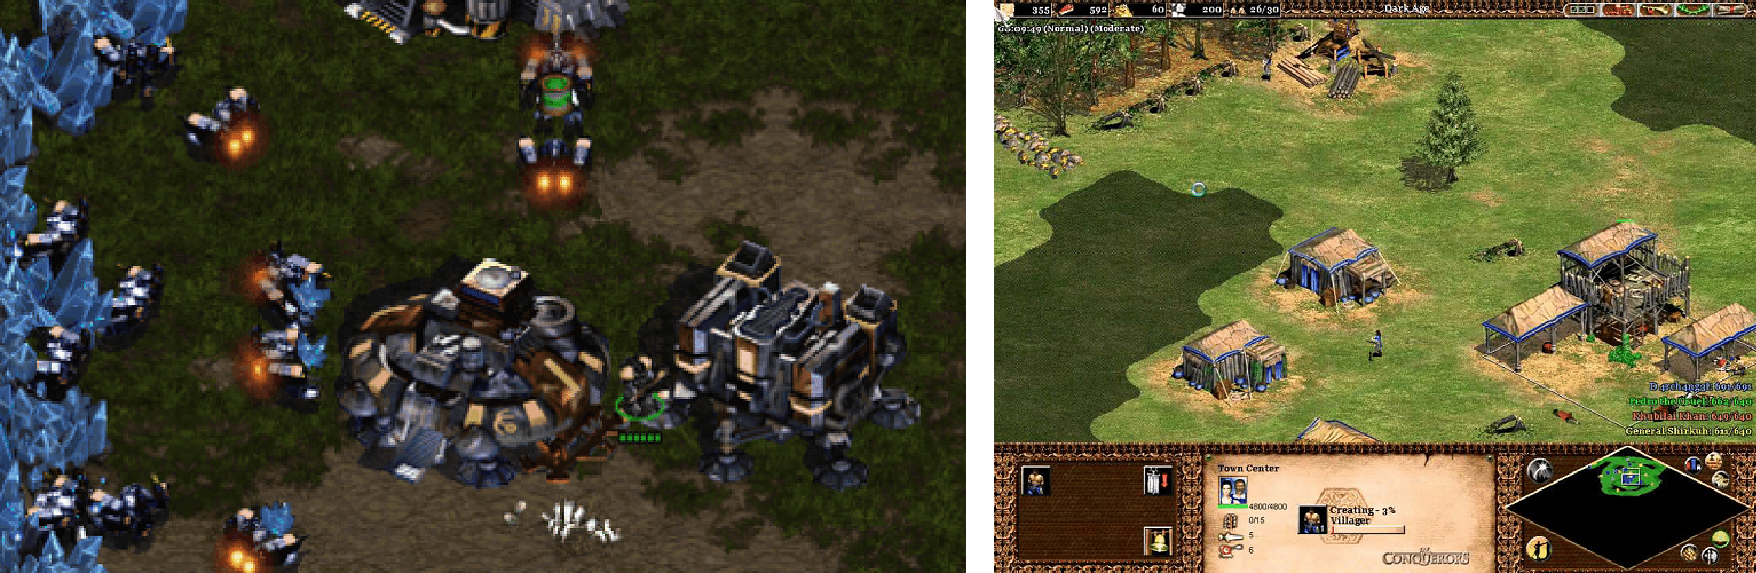
\includegraphics[width=1.0\textwidth]{photos/horizontal_rts.pdf}
	\end{center}
	\caption{Na zgornjih dveh slikah sta predstavljeni igra StarCraft (levo) in Age of Empires II (desno). 
		Obe igri sta prikazani v začetku igre, kjer sta na slikah vidni glavni hiši, delavci, viri surovin (minerali, rude zlata, drevesa ipd.).
		Pri igri Age of Empires II je viden zemljevid, kjer zasenčenost predstavlja neraziskani del. 
		Bodimo pozorni, da izvajanje določenih akcij poteka več časa, saj na primer delavci pri igri StarCraft vračajo mineralno rudo več časovnih enot, pri igri Age of Empires II pa se več časovnih enot urijo delavci.}
	\label{picRtsGames}
\end{figure}

Razlike realno-časovnih iger v primerjavi s tradicionalnimi namiznimi igrami je dobro opisal Santiago Ontañon v raziskovalnem delu Pregled učenja umetne inteligence na realno-časovnih strateških igrah in tekmovanja v igri StarCraft~\cite{survey_real_time_strategy_ai_research_starcraft}.
Te razlike so naslednje:
\begin{itemize}
	\item izvajanje akcij v istem časovnem intervalu, ki lahko trajajo več časovnih intervalov;
	\item odločitev akcij v krajšem časovnem obdobju, saj se za razliko od šaha, kjer ima igralec na voljo več minut za izbiro poteze, v igri, kot je npr. StarCraft, stanje igre zamenja 24-krat na sekundo;
	\item igre so lahko vidne le na področjih, kjer je igralec že raziskal določeno področje in imajo nanj vpogled igralčeve figure;
	\item večina iger ni determinističnih, ampak imajo akcije verjetnost uspeha;
	\item kompleksnost raziskovalnega prostora je veliko večja.
\end{itemize}
\noindent
Zaradi teh razlik so nastopili razni izzivi:
\begin{itemize}
	\item planiranje: Realno-časovne strateške igre imajo običajno večji raziskovalni prostor od tradicionalnih namiznih iger, kar prepreči globlje raziskovanje stanj iger. 
	Kot bomo pozneje pregledali, se igre zato abstrahirajo na več nivojev.
	Višji kot je nivo, bolj dolgoročni so cilji, kot na primer gradnja ekonomije, na nižjem nivoju pa so kratkotrajnejši cilji, kot na primer premik posamezne figure ipd.
	\item učenje: Učenje igranja igre lahko poteka na način predhodnega učenja, ki uporablja posnetke že odigranih iger, in na način učenja v igri, ki uporablja spodbujevalno učenje in modeliranje nasprotnika.
	\item negotovost: Negotovost nastane zaradi nevidnosti nasprotnikovih figur in njegovih potez v vsakem trenutku. 
	Ne moremo določiti, katero akcijo bo nasprotnik izvedel, zato je potrebna izgradnja drevesa, ki nam pove največjo verjetnost izbrane nasprotnikove akcije v določenem stanju igre.
	\item prostorsko in časovno razumevanje: Prostorsko razumevanje je usmerjeno k postavljanju stavb in pozicije vojske za obrambo in napad, medtem ko je časovno razumevanje usmerjeno k ugotavljanju časovne primernosti izdelave določenih figur, ki so primerne za izboljšavo igralčeve ekonomije, tehnološkega drevesa ali časa napada ipd.
	\item izkoriščanje znanja domen: V tradicionalnih igrah, kot je npr. šah, se lahko zanašamo na dobre ocenjevalne funkcije in na algoritem alpha-beta ter tabele s popolno informacijo o končnicah z malo figurami (ang. tablebases).
	V realno-časovnih strateških igrah ni jasno, kako lahko računalniški nasprotniki uporabijo domenska znanja iz posnetkov iger, zato se razvijalci tovrstnih iger bolj osredotočajo na izgradnjo več različnih taktik, med katerimi se odloča računalniški nasprotnik na podlagi hevristike.
	\item razdelitev nalog (prikazano na Sliki~\ref{picRazdelitevNalog}): Večje in zahtevnejše naloge so razdeljene na manjše, ki jih uvrščamo v več nivojev glede na abstrakcijo.
	\begin{itemize}
		\item Strategija je najvišji nivo abstrakcije, ki zajema okrog 3-minutna planiranja in vse figure ki jih igralec nadzoruje.
		\item Taktika je implementacija trenutne strategije (pozicija vojaških enot, stavb. 30-sekundno planiranje).
		\item Reakcijska kontrola je implementacija taktike, ki je osredotočena na posamezno figuro.
		\item Analiza terena se osredotoča na strnjena območja in na višinsko prednost.
		%\item Pridobivanje znanja je naloga s katero pridobivamo informacije o taktiki nasprotnika.
	\end{itemize}

	\begin{figure}[t!]
		\begin{center}
			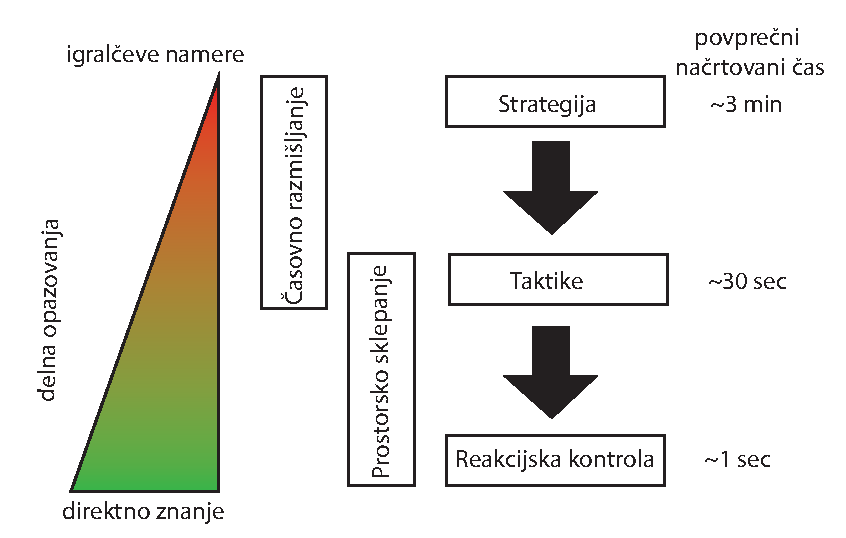
\includegraphics[width=0.8\textwidth]{photos/RazdelitevNalog.pdf}
		\end{center}
		\caption{Razdelitev nalog glede na čas reakcije in abstrakcije nalog. 
			Prikazani so nivoji odločanja glede na časovni razpon, kjer se negotovost akcij povečuje s povečevanjem ciljnega časa, za kar moramo igro pravilno abstrahirati na taktike in strategije. 
			Tem lahko lažje sledimo kakor posameznim taktikam osredotočenim na figuro, saj predstavljajo strnjene zbirke krajših akcij. }
		\label{picRazdelitevNalog}
	\end{figure}
\end{itemize}

\section{Strategija}
V strateških igrah je velikokrat uporabljen pristop direktnega kodiranja strategije, ki uporabljajo končne avtomate, kjer lahko razbijemo delovanje na več stanj, kot so napadanje, nabiranje surovin, popravilo itd., in hitro menjavanje med njimi. 
Direktno kodiranje prinese dobre pričakovane rezultate, vendar se lahko človeški igralec nauči te strategije in tako računalniškega agenta hitro porazi.
Planirani pristopi ponujajo večjo prilagodljivost kot direktno kodirani.
\section{Taktika}
Taktika spada pod neposrednejši nadzor figur kakor strategija in je bolj osredotočena na kontrolo določenih točk na mapi, zmago posameznih bitk in iskanje ožin, kjer je nasprotnik šibkejši. 
Taktika temelji na analizi terena, ki ga lahko razbijemo na kompozicijo ožin.

Razbiranje strategije in taktike je za algoritme umetne inteligence težja naloga od nadzorovanja posameznih figur, saj potrebuje višji nivo abstrakcije prostora, figur in akcij kot za izbiro posameznih nizkonivojskih akcij, zato smo se v sklopu diplomske naloge odločili za nadzorovanje figur na nižjem nivoju abstrakcije (nivo reakcijske kontrole).

\section{Abstrakcija prostora}
Za primer abstrakcije prostora vzemimo strateško realno-časovno video igro, kjer figuro spremlja vsaka prikazana točka na prikazovalniku.
V tem primeru bi bilo že prepoznavanje figure za algoritem zahtevno. 
Še zahtevnejši bi pa bil zapis akcij, kot npr. premik, saj se lahko ta figura, opisana z zapisom točk na prikazovalniku, premakne na poljubno dovoljeno mesto.
Zato je primernejše, da figure in njihove premike obravnavamo na višjih ravneh abstrakcije igre~\cite{uriarte2015automatic}.
Figuro lahko predstavimo na lažji način, kjer nas zanima le majhna množica atributov.
Posamezne figure vojaških enot lahko združujemo v večje skupine, katere potem obravnavamo in upravljamo kot en osebek.
Te skupine vojaških enot je potrebno pravilno razporediti na razne strateške točke, ki nam zagotavljajo prednost pred nasprotnikom.
V ta namen lahko razgradimo zemljevid igre glede na ožine in prestope iz višjega na nižji del terena.
Z zgrajenim zemljevidom lahko postavimo figure na razne strateške točke~\cite{uriarte2014game}.

V našem delu smo zemljevid razbili kar na kvadratno mrežo 8~x~8 ali 6~x~6, saj ne vsebuje nobenih ožin in nedostopnih mest.
Imamo majhno število posameznih enot (npr. vojaško enoto), ki jih lahko v video igro apliciramo kot skupek enot, kot smo to opisali zgoraj (npr. skupino vojaških enot).

Abstrakcija prostora poteka težje, če igra vsebuje dejavnike negotovosti, kot je na primer prekrivanje zemljevida z meglo (ang. fog of war), kjer igralec nima podatka o lokaciji, številu in tipih nasprotnikovih figur in njihovih potezah v vsakem trenutku~{\cite{ciancarini2010monte}}. 
Napoved nasprotnikovih potez je tako veliko težja, tako da vsi algoritmi s tako negotovostjo ne delujejo.
Mi smo se za diplomsko nalogo odločili, da imata oba računalniška agenta popoln vpogled na stanje igre in nasprotnikove akcije, saj je to privzeto delovanje izbranega algoritma AlphaZero.

V igri, kot je npr. StarCraft, lahko posamezno vojaško enoto premaknemo na poljubno koordinato na zemljevidu pod pogojem, da je ta koordinata dosegljiva z vidika algoritma za iskanje poti.
Te koordinate premika lahko segajo tudi v neznane dele zemljevida, ki so lahko že zasedene z nasprotnikovo arhitekturo, zato lahko premikanje poenostavimo na sosednja polja.
Napad nasprotnikovih enot, nabiranje zlatnikov ipd. lahko omejimo na izvajanje akcij znotraj določenega polja na najbližjo figuro.
Na primer, vojaška enota lahko napade najbližjo nasprotnikovo enoto znotraj polja, v katerem je ta naša vojaška enota.
V našem primeru, kot bomo pojasnili pri poglavju opis pravil igre~\ref{chpravilaigre}, ne moremo postaviti več figur na isto polje, zato so akcije, kot so napad ali nabiranje zlatnikov, omejene na sosednja polja.

Prav tako smo poenostavili izvajanje akcij, saj smo privzeli izmenjujoče izvajanje potez dveh igralcev.
To je namreč pogoj implementacije igre z algoritmom AlphaZero.
Oba igralca morata biti obveščena o trenutnem stanju igre, drugače lahko nastopi na primer akcija premika dveh enot na isto polje na šahovnici, kar v naši strateški igri ni dovoljeno.

%%%%%%%%%%%%%%%%%%%%%%%%%%%%%%%%%%%%%%%%%%%%%%%%%%%%%%%%%%%%%%%%%%%%%%%%%%%%%%%%%%%%%%%%%%%%%%%%%%%%%%%%%%%%%%%%%%%%%%%%
%%%%%%%%%%%%%%%%%%%%%%%%%%%%%%%%%%%%%%%%%%%%%%%%%%%%%%%%%%%%%%%%%%%%%%%%%%%%%%%%%%%%%%%%%%%%%%%%%%%%%%%%%%%%%%%%%%%%%%%%
%%%%%%%%%%%%%%%%%%%%%%%%%%%%%%%%%%%%%%%%%%%%%%%%%%%%%%%%%%%%%%%%%%%%%%%%%%%%%%%%%%%%%%%%%%%%%%%%%%%%%%%%%%%%%%%%%%%%%%%%
%%%%%%%%%%%%%%%%%%%%%%%%%%%%%%%%%%%%%%%%%%%%%%%%%%%%%%%%%%%%%%%%%%%%%%%%%%%%%%%%%%%%%%%%%%%%%%%%%%%%%%%%%%%%%%%%%%%%%%%%
%%%%%%%%%%%%%%%%%%%%%%%%%%%%%%%%%%%%%%%%%%%%%%%%%%%%%%%%%%%%%%%%%%%%%%%%%%%%%%%%%%%%%%%%%%%%%%%%%%%%%%%%%%%%%%%%%%%%%%%%

\chapter{Predstavitev algoritma AlphaZero}
\label{alphazero}
\section{Zgodovina}

Igranje iger je popularno področje znotraj vede o umetni inteligenci. 
Desetletja je bil za raziskovalce s področja umetne inteligence podvig razviti program za igranje šaha.
Danes so najboljši algoritmi za igranje šaha nepremagljivi celo za svetovnega prvaka.
Ti algoritmi temeljijo na preiskovanju prostora več milijonov šahovskih pozicij in metodah, ki temeljijo na pravilih.
Za razliko od teh programov je bil eden izmed prvih programov Checkers za igranje igre dama (ang. checkers) (Samuel 2000~{\cite{samuel2000some}}), ki se je naučil igranja z metodami samo-igranja in strojnega učenja in ne npr. na metodah, ki temeljijo na pravilih.

Pri tradicionalnih namiznih igrah je vejitveni faktor akcij relativno majhen in je lažje oceniti končno pozicijo iz danega stanja~\cite{wiki:AlphaGo}.
Rečeno je bilo, da za igre, kot je npr. Go, ki ima znatno večje število možnih pozicij ($10^{171}$) v primerjavi s šahom (ki ima med $10^{40}$ in $10^{46}$ pozicij~\cite{chinchalkar1996upper}~\cite{steinerberger2015number}), ne bo možno ugotoviti vrednosti končnega stanja še nekaj desetletij.
Algoritem AlphaGo~\cite{silver2016mastering} je naredil preboj s tem, da uporablja metodo globokega spodbujevalnega učenja in algoritem drevesno preiskovanje Monte Carlo. 
Oktobra 2016 je premagal profesionalnega Go igralca na podlagi učenja na domenskem znanju iger, ki so jih odigrali eksperti.
Ti sistemi so temeljili na predznanju ekspertov za učenje in ocenitev modela, kar pomeni, da ob igranju novih iger posnemajo ekspertovo igranje igre.

Leto za tem je bil razvit algoritem AlphaGo Zero~\cite{silver2017mastering}, ki opisuje pristop k učenju brez domenskega znanja ekspertov, ampak uporablja metodo samo-igranja (učenje, predstavljeno na Sliki~\ref{picCompareGo}). 
Novi model je premagal algoritem AlphaGo, kar predstavlja odlične rezultate z vidika, da AlphaGo Zero pri učenju ne potrebuje usmerjanj s človeškim predznanjem.
Računalniški agenti se lahko tako naučijo reševanja problema brez človeških ekspertov, ki pogostejše delajo napake zaradi utrujenosti ali površnosti in nimajo takojšnega vpogleda na celotno zbirko učne množice.

\begin{figure}[h!]
	\begin{center}
		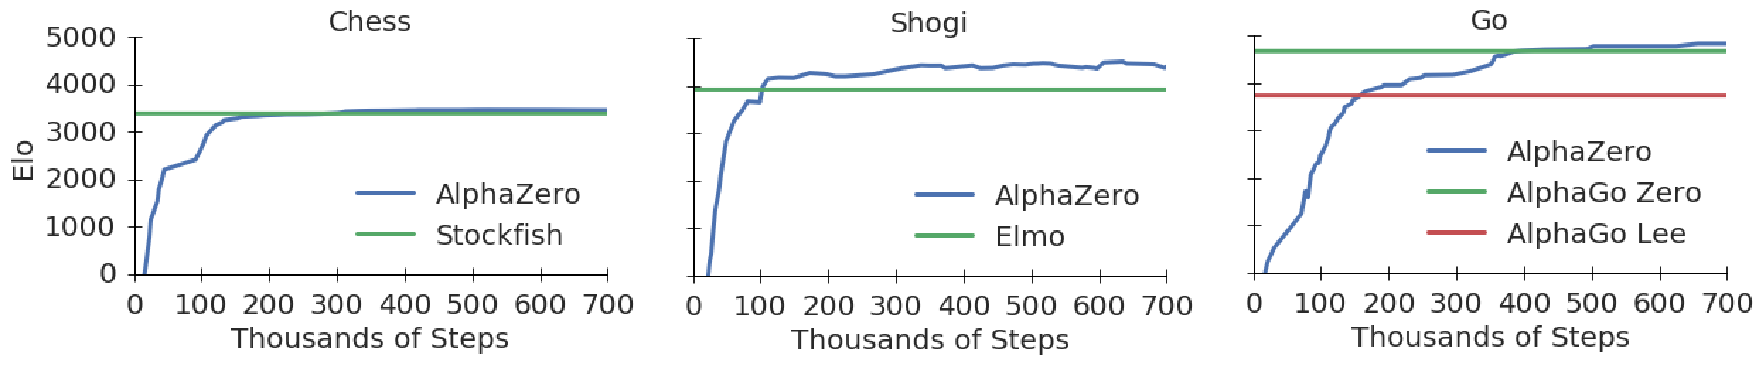
\includegraphics[width=1\textwidth]{photos/go.pdf}
	\end{center}
	\caption{Predstavitev igranja iger z naučenim algoritmom AlphaZero s 700,000 iteracijami, kjer je čas za napoved akcije 1 sekunda.
		Na levi sliki je prikaz igranja šaha proti programu Stockfish iz leta 2016, na srednji sliki igranje proti programu Elmo iz leta 2017 v igri shogi, na desni igranje igre Go proti programoma AlphaGo Lee in AlphaGo Zero~{\cite{silver2017mastering}}.
 }
	\label{picCompareGo}
\end{figure}
\noindent
Delovanje algoritma AlphaGo Zero lahko opišemo v naslednjih korakih~\cite{guid}:
\begin{itemize}
	\item miselno odigraj igro z raziskovanjem neodkritega, pri čemer upoštevaj nasprotnikove akcije,
	\item pri soočenju z neznano pozicijo oceni njeno vrednost in popravi ocene pozicij, ki so vodile do trenutne pozicije,
	\item po prenehanju razmišljanja odigraj potezo, ki je najbolj obetavna,
	\item po koncu igre preglej vse pozicije, kjer si se za pozicije narobe odločil, in jih popravi.
\end{itemize}

\noindent
Za tem je bil razvit algoritem AlphaZero, ki kot temelj vzame ideje AlphaGo Zero in posploši model za poljubne igre, kot so na primer šah, shogi, Go.
Algoritem za delovanje potrebuje samo pravila igre, na podlagi katerih se uči igranja z globokimi nevronskimi mrežami in tabula rasa algoritmom za spodbujevalno učenje.
Zaradi te posplošitve algoritma ga lahko preslikamo na našo RTS igro.
Algoritem AlphaZero je drugačen od AlphaGo Zero v tem, da igre pri AlphaGo Zero nastanejo z igranjem vseh posameznih modelov prejšnjih iteracij, na kar se je moč modela izračunala proti najboljšim igralcem, medtem ko AlphaZero samo hrani eno nevronsko mrežo, ki se stalno posodablja, namesto da čaka iteracijo, da se konča.

\section{Potek učenja}
\label{potekUcenja}
AlphaZero se uči verjetnosti in ocenitve končnega stanja izključno z igranjem proti samemu sebi. 
To potem uporabi pri preiskovanju z glavno namensko metodo drevesnim preiskovanjem Monte Carlo, da razišče drevo stanj za akcijo.
Drevo preišče prostor in vrne verjetnost zmage pri izbiri določene akcije iz trenutnega stanja imenovano $Pi$ in oceno končnega stanja iz trenutnega stanja imenovanega {$V\in\mathbb{R}[-1, 1]$ (poraz, zmaga).
AlphaZero izvede več serij igranja iger proti svojim nasprotnikom, ki predstavlja zdajšnji najboljši model igranja.
Rezultat igranja igre je lahko -1 za poraz, +1 za zmago in 0 za neodločeno.
Po vsaki seriji učenja, se izvede proces igranja iger dveh naučenih modelov, kjer oba igrata drug proti drugemu nekaj iger, nato pa se določi zmagovalni model, ki sedaj postane najboljši model, če je razlika v številu zmag večja za nek faktor.
V našem primeru je bil ta faktor 60\%.

Parametri nevronske mreže so za tem popravljeni, da minimizirajo napako med napovedjo stanja nevronske mreže in dejanskim rezultatom igre ter maksimizirajo podobnost napovedi potez nevronske mreže z dejanskimi vrednostnimi akcij, ki so rezultat drevesnega preiskovanja Monte Carlo (ang. Monte Carlo tree search; MCTS). 
Parametri se nastavijo z gradientnim spustom na funkcijo izgube, ki sešteje srednjo kvadratno napako (ang. mean-squared error; MSE) in prečne entropije (ang. cross entropy).
Nevronska mreža sprejme učne množice stanja iger in vrne izravnan vektor napovedi akcij v trenutnem stanju, označeno s $Pi$, in napoved zmage, označeno z $V$.

\begin{figure}[h!]
	\begin{center}
		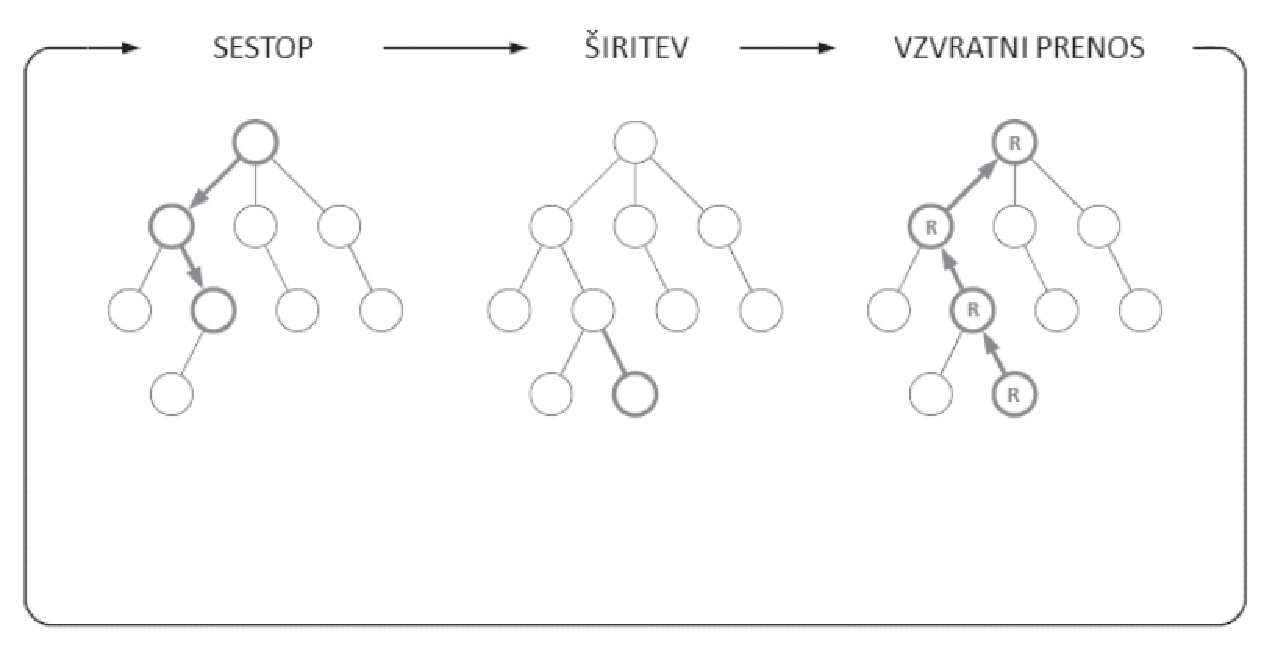
\includegraphics[width=0.8\textwidth]{photos/modifiedMCTS.pdf}
	\end{center}
	\caption{Na sliki je prikazano delovanje algoritma MCTS pri izvedbi algoritma AlphaZero, ki ga uporabljamo v diplomski nalogi. 
		MCTS ne uporablja postopka odigravanja stanj do konca igre, ampak izvede določeno število iteracij iskanja z raziskovalno funkcijo (glej Izrek~\ref{iz:1}, ki predstavlja računanje verjetnosti zmage pri določeni akciji v algoritmu MCTS).}
	\label{modifiedMCTS}
\end{figure}

Uporaba algoritma MCTS je v tej implementaciji algoritma AlphaZero drugačna kakor v splošni uporabi.
Število iteracij je veliko manjše, kakor v njegovi klasični uporabi, kjer je število iteracij več sto tisoč. 
MCTS pripomore k izboljšavi napovedi stanja, ki ga vrne nevronska mreža z raziskovanjem prostora.
Algoritem ne uporablja simulacij za pridobitev končnega stanja igre, vendar samo izboljša napoved stanja, ki ga vrne nevronska mreža.

Vozlišče oziroma stanje ($s$), ki še ni bilo obiskano oziroma ni bila izvedena akcija ($a$), se vzpostavi z napovedjo nevronske mreže in za tem vzvratno propagira napoved stanja U($s$, $a$) (glej Izrek~{\ref{eq:mctsFormula}}).
Če je vozlišče končno stanje igre, vzvratno propagira končno stanje.
MCTS v tem primeru izvede par sto iteracij (v našem primeru 30-50) in ne več tisoč, kot jih izvajajo drugi algoritmi.
V sklopu diplomske naloge govorimo o MCTS iskanjih in ne odigravanjih, saj jih ta ne vpeljuje (glej Sliko~\ref{modifiedMCTS}).

\begin{izrek}
	\label{iz:1}
	Pričakovana vrednost akcije v določenem stanju igre U($s$,~$a$) predstavlja pričakovano nagrado ob izbiri akcije ($a$) v danem stanju igre ($s$) Q($s$,~$a$), kateri je prišteta napoved nagrade v tem stanju P($s$,~$a$) ob izbiri akcije v danem stanju, ki ga vrne nevronska mreža, pomnoženo s raziskovalnim faktorjem in korenom števila vseh obiskov stanja igre v primerjavi s števili obiskov danega vozlišča.
	\begin{equation}
	U(s, a) = Q(s, a) + c_{p,uct}P(s, a)\dfrac{\sqrt{\sum{N(s)}}}{1+N(s, a)}
	\label{eq:mctsFormula}
	\end{equation}
\end{izrek}
\noindent
Glavno učenje algoritma poteka z igranjem iger, ki se za razliko od algoritma MCTS odigrajo do konca in se dodajo v seznam učnih primerov.
Na koncu vsake iteracije igranja epizod iger se nevronska mreža uči na podlagi teh učnih primerov.
Za tem preveri moč novo naučenega modela z igranjem proti starejši različici modela.
Novi model se shrani samo, če je boljši od starejšega za določen odstotek.

%%%%%%%%%%%%%%%%%%%%%%%%%%%%%%%%%%%%%%%%%%%%%%%%%%%%%%%%%%%%%%%%%%%%%%%%%%%%%%%%%%%%%%%%%%%%%%%%%%%%%%%%%%%%%%%%%%%%%%%%
%%%%%%%%%%%%%%%%%%%%%%%%%%%%%%%%%%%%%%%%%%%%%%%%%%%%%%%%%%%%%%%%%%%%%%%%%%%%%%%%%%%%%%%%%%%%%%%%%%%%%%%%%%%%%%%%%%%%%%%%
%%%%%%%%%%%%%%%%%%%%%%%%%%%%%%%%%%%%%%%%%%%%%%%%%%%%%%%%%%%%%%%%%%%%%%%%%%%%%%%%%%%%%%%%%%%%%%%%%%%%%%%%%%%%%%%%%%%%%%%%
%%%%%%%%%%%%%%%%%%%%%%%%%%%%%%%%%%%%%%%%%%%%%%%%%%%%%%%%%%%%%%%%%%%%%%%%%%%%%%%%%%%%%%%%%%%%%%%%%%%%%%%%%%%%%%%%%%%%%%%%
%%%%%%%%%%%%%%%%%%%%%%%%%%%%%%%%%%%%%%%%%%%%%%%%%%%%%%%%%%%%%%%%%%%%%%%%%%%%%%%%%%%%%%%%%%%%%%%%%%%%%%%%%%%%%%%%%%%%%%%%

\chapter{Opis pravil igre}
\label{chpravilaigre}

Igro smo opisali po Surag Nairjevi predlogi za igro AlphaZero, ki je na voljo na spletem gostovanju GitHub~\cite{alphazerogeneral}.
Strateško igro smo dodali kot modul, ki mora vsebovati definicijo igre in njena pravila, igralce, vizualizacijo in izgradnjo modela.

Igra je določena s kvadratno mrežo 8 x 8, kjer polje lahko vsebuje največ eno figuro.
Ostale igre, ki so napisane za to različico AlphaZero izvedbe, kot na primer štiri v vrsto, gomoku, othello, tri v vrsto, vsebujejo črno-bele figure.
Zakodirane so lahko z eno številko: -1 za igralca -1, +1 za igralca 1 in 0, če je polje prazno.
Pri teh igrah je dimenzija kodiranja 2-dimenzionalna, kjer dimenzije predstavljajo višino in širino igralne plošče, zapis v polju pa je številka igralca.
Pri RTS igrah moramo poleg igralca vedeti, komu ta figura pripada in stanje te figure (npr. trenutno število življenjskih točk in njen tip).
Zato je prostor kodiranja 3-dimenzionalen, kjer je tretja dimenzija vektor stanja figure na polju.
Če bi dovolili, da na posamezno polje spada več figur, se dimenzija ponovno poveča za 1.

Naš prvi poskus opisa igre je zelo spremenil Surag-Nairjevo implementacijo algoritma AlphaZero, saj smo stanja igre skozi algoritem prenašali ne-numerično~\cite{objectAlphaZero}.
Hoteli smo ohraniti združljivost z ovojnico algoritma, za katerega implementiramo svojo igro kot modul, kar je nenumerični zapis igre preprečil.
Kompleksnejša implementacija igre je povzročila počasnejše igranje in učenje iger, saj je bilo preverjanje akcij počasnejše, zato smo igro morali napisati ponovno.

\section{Stanje igre}
\label{stanjeigre}
V tem razdelku bomo opisali zapis posamezne figure, njihove akcije, kaj naredijo ter tip kodiranja stanja igre, ki ga potem sprejme nevronska mreža.

Igro smo opisali na način, da je čim bolj skladen z algoritmom AlphaZero, kot tudi da je njena aplikacija v video igro dovolj primerljiva z obstoječimi strateškimi video igrami, kot je npr. StarCraft.
Tako smo opisali nekaj preprostih pravil, ki jih ta igra upošteva:
\begin{itemize}
	\item figure se ne požirajo: Vojaške figure ne napadejo drugih figur tako, da bi se ob akciji napada figura postavila na polje nasprotnikove figure, in s tem prepisala nasprotnikovo figuro in jo s tem uničila (primerjava je prikazana na Sliki~\ref{picPoziranjeFigur}). 
	Vse figure imajo določeno število življenjskih točk, ki ga vojaške figure v večih korakih zmanjšajo z napadom.
	\item ena figura na polje: S tem pravilom ni možno blokiranje figur na način, da se figura postavi na polje zlata in blokira nasprotnikovo figuro, da ga nabere.
	\item Igralec izgubi igro, če izgubi vse figure. Več o ustavitvenih pogojih je napisano spodaj v razdelku~\ref{sKonecIgre}.
	\item Nabiranje zlatnikov je enkratna operacija, ki poteka podobno kot pri igri StarCraft, kjer mora figura pristopiti do polja zlata, zlatnike pobrati, se ponovno premakniti po šahovnici do glavne hiše in vanjo vrniti nabrane zlatnike.
	Nabiranje zlatnikov v tem primeru ne poteka tako, da se figura pomakne do polja zlata in s tem igralec avtomatično prične pridobivati zlatnike, brez da bi jih figura vračala v glavno hišo.
\end{itemize}

\begin{figure}[h!]
	\begin{center}
		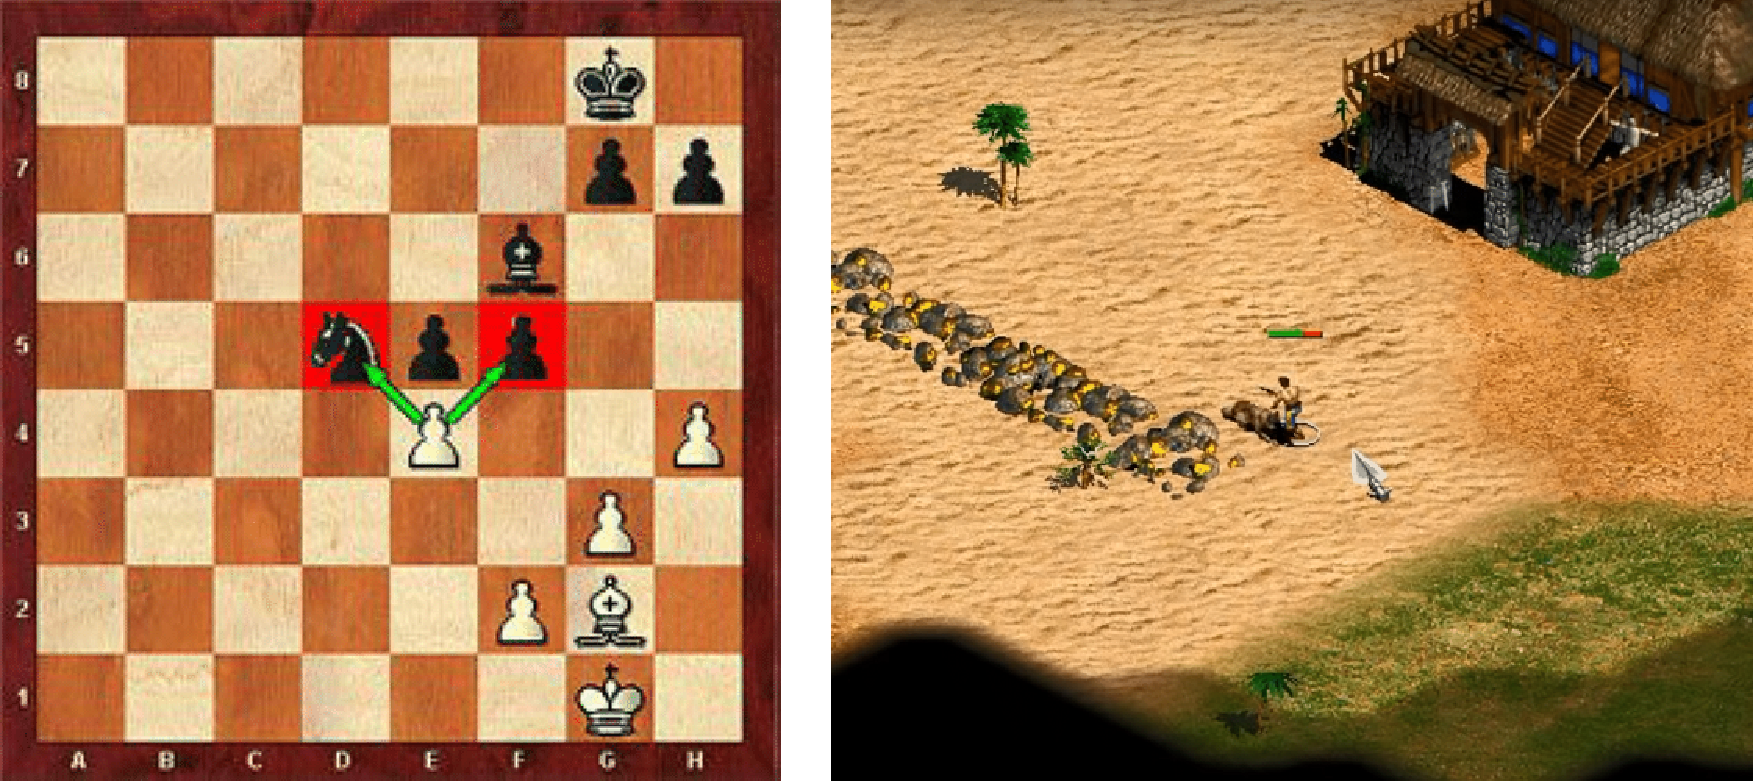
\includegraphics[width=1\textwidth]{photos/horizontal_health.pdf}
	\end{center}
	\caption{Na levi sliki je prikaz požiranja figur v igri šah, kjer se figura kmet lahko premakne na eno izmed dveh diagonalnih polj in s tem uniči trenutno nasprotnikovo figuro na tem polju. 
		Na desni sliki je prikaz vojskovanja delavca z volkom v igri Age of Empires II, kjer se figurama odšteva število življenjskih točk med napadanjem, ki lahko traja več časovnih enot. }
	\label{picPoziranjeFigur}
\end{figure}
\noindent
Sprva moramo opisati figure, ki bodo imele določeno vlogo v igri. 
Nabor figur je majhen, saj nočemo, da preiskovalni prostor prehitro postane prevelik.

\begin{table}
	\begin{center}
		\begin{tabular}{p{0.2\linewidth}|p{0.7\linewidth}}
			Ime figure        & {\tt Opis} \\ \hline
			{\tt polje zlata} & Vir surovin, ki predstavljajo denar v igri, s katerim lahko igralec gradi nove stavbe in uri nove figure. 
								Vir zlata je neomejen in ne more biti uničen. \\
			{\tt delavec}     & Figura, namenjena gradnji stavb in nabiranju zlatnikov. \\
			{\tt vojašnica}   & Stavba, namenjena urjenju vojaških figur. \\
			{\tt vojak}       & Figura, namenjena napadanju nasprotnikovih figur. \\
			{\tt glavna hiša} & Stavba, namenjena urjenju delavcev in odložišče zlatnikov. \\
		\end{tabular}
	\end{center}
	\caption{Določitev figur in njihovih namenov v igri. Definirali smo samo 5 figur, med katerimi je polje zlata nevtralna, saj je igralec ne more nadzorovati. }
	\label{tableFiguresDescription}
\end{table}

Realizirali smo atribute figur. 
Pomembno je, da so ti atributi numerični, da lahko podamo stanje igre kot N-dimenzionalen vektor, ki ga nevronska mreža lahko sprejme in se iz teh numeričnih podatkov uči.
Pomembno je, da ima vsako polje na šahovnici enako število atributov, tudi če je to polje prazno.

\begin{table}
	\begin{center}
		\begin{tabular}{p{0.2\linewidth}|p{0.7\linewidth}}
			Ime kodirnega polja                      & {\tt Opis} \\ \hline
			{\tt ime igralca}                        & Določa igralca, kateremu ta figura pripada. 
			 										   Igralec lahko nadzoruje samo svoje figure, izvaja akcije na svojih figurah in napada nasprotnikove figure. \\
			{\tt tip figure}                         & Atribut predstavlja numerično predstavitev tipa figure, kot je na primer polje zlata, delavec ipd.
													   Stanje igre potrebuje zapise tipov figur na poljih, da program ve, katere akcije tem figuram pripadajo, koliko je strošek izdelave nove figure tega tipa in njenih življenjskih točk.\\
			{\tt število življenjskih točk}          & Zapisuje trenutno število življenjskih točk.
													   Število se lahko povečuje do določene zgornje meje z akcijo zdravi in znižuje z napadom nasprotnikove figure. Če je število točk 0 ali manj, je figura odstranjena s šahovnice. \\
			{\tt nosi zlatnike}                      & Poseben atribut za figuro delavec, ki predstavlja vrednost 1, če figura nosi zlatnike, in 0, če jih ne nosi.
													   Upošteva se pri nabiranju in vračanju zlatnikov, kjer se ti dve akcije ne zgodita v roku ene poteze, ampak se mora stanje prenašati skozi več potez. \\
			{\tt denar}                              & Trenutna količina zbranega denarja za posameznega igralca.
													   To polje se ob spremembi količine denarja spremeni v vseh figurah tega igralca. \\
			{\tt čas igranja}                        & To polje predstavlja, koliko potez se je v trenutni igri že izvedlo.
													   Atribut je prisoten v vseh poljih in se spremeni v vseh poljih šahovnice, ko se izvede nova akcija. \\
		\end{tabular}
	\end{center}
	\caption{Definicija in opis kodirnikov stanja igre, s katerimi je predstavljeno vsako polje na šahovnici. Več o kodiranju teh polj si bomo pogledali v sekciji kodiranje~\ref{kodiranja}.}
	\label{tableEncoders}
\end{table}

Poseben primer je figura polje zlata, ki ne pripada nobenemu igralcu v večini RTS iger. 
V tem primeru smo podali vsakemu igralcu svoje polje zlata, da je igra simetrična in nevronska mreža ne interpretira tega polja kot praznega.
Figuri polje zlata se ne spreminja atribut zdravja, saj jo ne moremo poškodovati. 
Zlatnikov je neomejeno število in ko igralec odloži zlatnike v glavno hišo, se vsem figuram tega igralca nastavi atribut zlatnikov na novo dobljeno vrednost, kar poveča število zlatnikov za tega igralca. 
Pri izgradnji nove stavbe ali urjenju figure se število zlatnikov zmanjša za vse figure tega igralca.

\section{Akcije}

\begin{figure}[h!]
	\begin{center}
		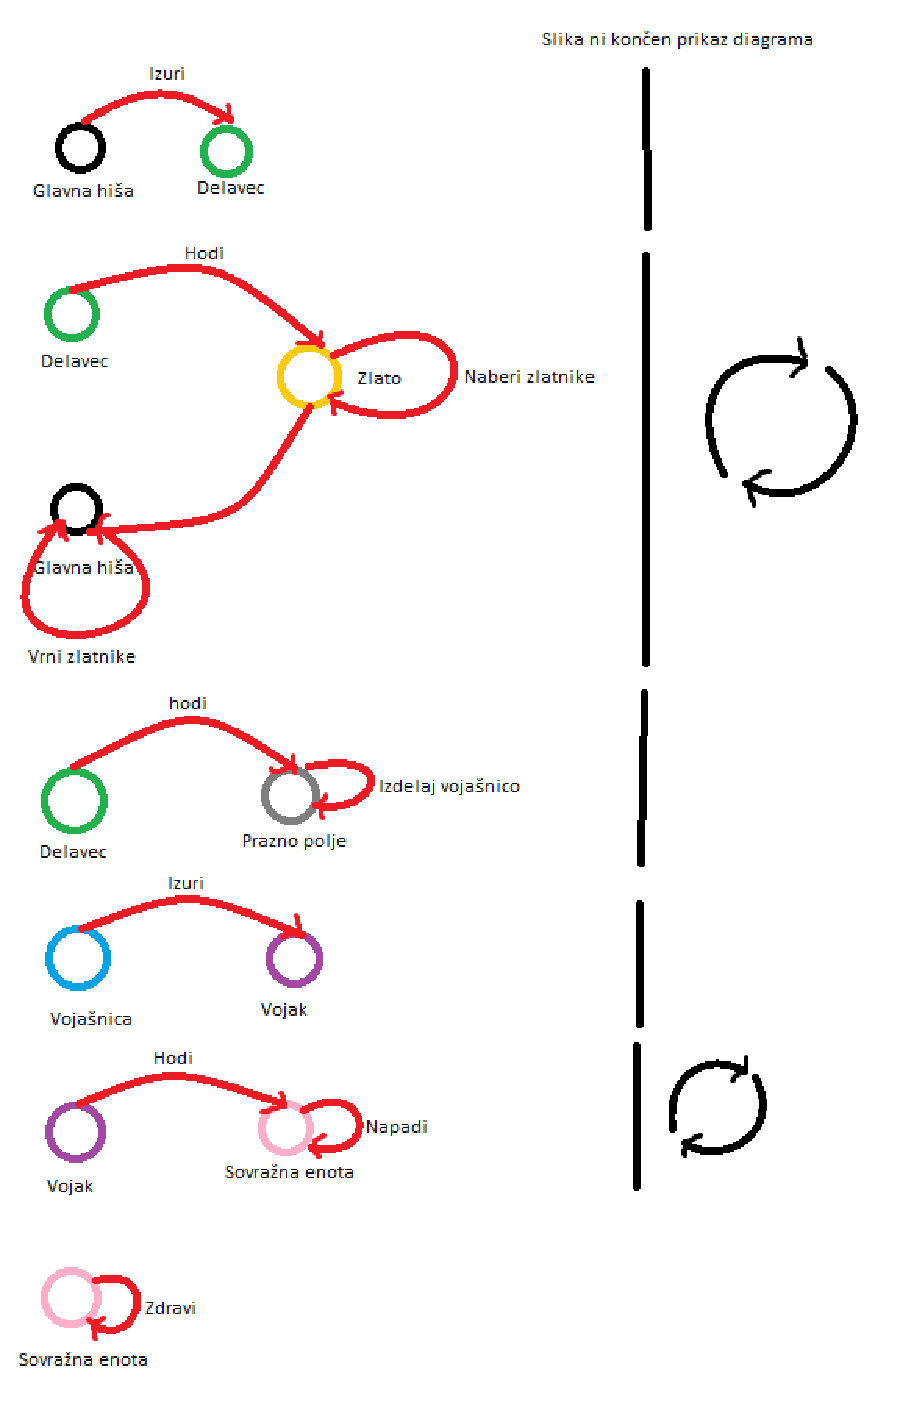
\includegraphics[width=0.9\textwidth]{photos/prikazAkcij.pdf}
	\end{center}
	\caption{Slika prikazuje diagram poteka možnih akcij in njihovih rezultatov ob določenih pogojih.}
	\label{picActions}
\end{figure}

Pri opisu pravil igre smo tudi določili akcije (glej Sliko~\ref{picActions}), ki jih igralčeve figure lahko izvajajo. 
Vsaka figura ne more izvajati vseh akcij. 
Na primer stavbe se ne morejo premikati, figure kot delavec in vojak pa ne morejo uriti novih figur (glej Tabelo~\ref{tabelfigures}).

\begin{table}
	\begin{center}
		\begin{tabular}{p{0.28\linewidth}|p{0.62\linewidth}}
			Ime akcije                          & {\tt Opis} \\ \hline
			{\tt premiki (4~smeri)}             & Figuri vojak in delavec se lahko premakneta na sosednje polje na šahovnici, če je to mesto prazno.
												  Premiki se lahko izvajajo samo v štirih smereh.\\
			{\tt naberi zlatnike (8~smeri)}     & Delavec lahko nabere zlatnike, če je v neposredni bližini figure polje zlata.
												  Zlatnike za tem drži pri sebi, pri čemer se nastavi zastavica nošenja zlatnikov na 1.\\
			{\tt vrni zlatnike (8~smeri)}       & Delavec vrne zlatnike, ki jih drži pri sebi, v glavno hišo, nakar se igralcu prišteje denar, delavcu pa ponastavi zastavica nošenja zlatnikov.\\
			{\tt napadi (4~smeri)}              & Vojak lahko napade nasprotnikovo figuro, če je ta v neposredni bližini, in jo rani za določen faktor. 
												  Če figuri ne preostane več življenjskih točk, je odstranjena s šahovnice. Če je bila uničena igralčeva zadnja figura, je igralec poražen.\\
			{\tt izuri delavca (4~smeri)}       & Glavna hiša lahko izuri novo figuro delavec, če ima dovolj denarja, nakar se igralcu odšteje denar.\\
			{\tt izuri vojaka (4~smeri)}        & Vojašnica lahko izuri novo figuro vojak, če ima dovolj denarja, nakar se igralcu odšteje denar.\\
			{\tt izgradi vojašnico (4~smeri)}   & Delavec lahko izgradi vojašnico na prazno mesto zraven njega, nakar se igralcu odšteje denar.\\
			{\tt izgradi glavno hišo (4~smeri)} & Delavec lahko izgradi glavno hišo na prazno mesto zraven njega, nakar se igralcu odšteje denar.\\
			{\tt zdravi (4~smeri)}              & Figura lahko zdravi sosednjo prijateljsko figuro, če ta nima polnega življenja, nakar se igralcu odšteje denar.\\
		\end{tabular}
	\end{center}
	\caption{Opis akcij, njihovih dejanj in pogojev, ki morajo biti izpolnjeni, da se akcija lahko izvrši.
		Nekatere akcije imajo 4 smeri izvajanja, kar pomeni, da bo npr. akcija izuri delavca dol povzročila, da se izuri delavec na južni strani glavne hiše.}
	\label{tableActions}
\end{table}

Vredno je izpostaviti akcijo nedejavnosti, ki v igri ni prisotna.
Izvedba te akcije konča potezo za trenutnega igralca in ne spremeni stanja igre.
Vpeljava te akcije bi bila smiselna pri nadzorovanju več figur v eni potezi, kjer lahko določene figure stojijo na mestu in s tem stražijo strateško točko ali pa varčujejo z zlatniki, s tem da vsakič ne izgradijo novo vojaško enoto.
V naši igri nadzorujemo samo eno figuro na potezo, tako da je ta akcija odvečna, saj podaljša čas učenja, saj se stanje igre spreminja počasneje.\\\\\\\\\\

Sprva smo določili nekatere izmed zgornjih akcij na način izbire prvega mesta med sosednjimi polji, ki ustreza akciji. 
Naslednje akcije so se izvajale po zaporedju vidnem na sliki~\ref{pickorakiPreverjanja}:
\begin{itemize}
	\item naberi zlatnike,
	\item vrni zlatnike,
	\item napadi,
	\item izuri delavca,
	\item izuri vojaka, 
	\item izgradi vojašnico,
	\item izgradi glavno hišo,
	\item zdravi.
\end{itemize}
\begin{verbatim}
koordinate = [(x - 1, y + 1),
              (x, y + 1),
              (x + 1, y + 1),
              (x - 1, y),
              (x + 1, y),
              (x - 1, y - 1),
              (x, y - 1),
              (x + 1, y - 1)]
for sosednji_x, sosednji_y in koordinate:
    # preveri pogoj akcije
    if (pogoj == ok):
        return sosednji_x, sosednji_y
\end{verbatim}

\begin{figure}[h!]
	\begin{center}
		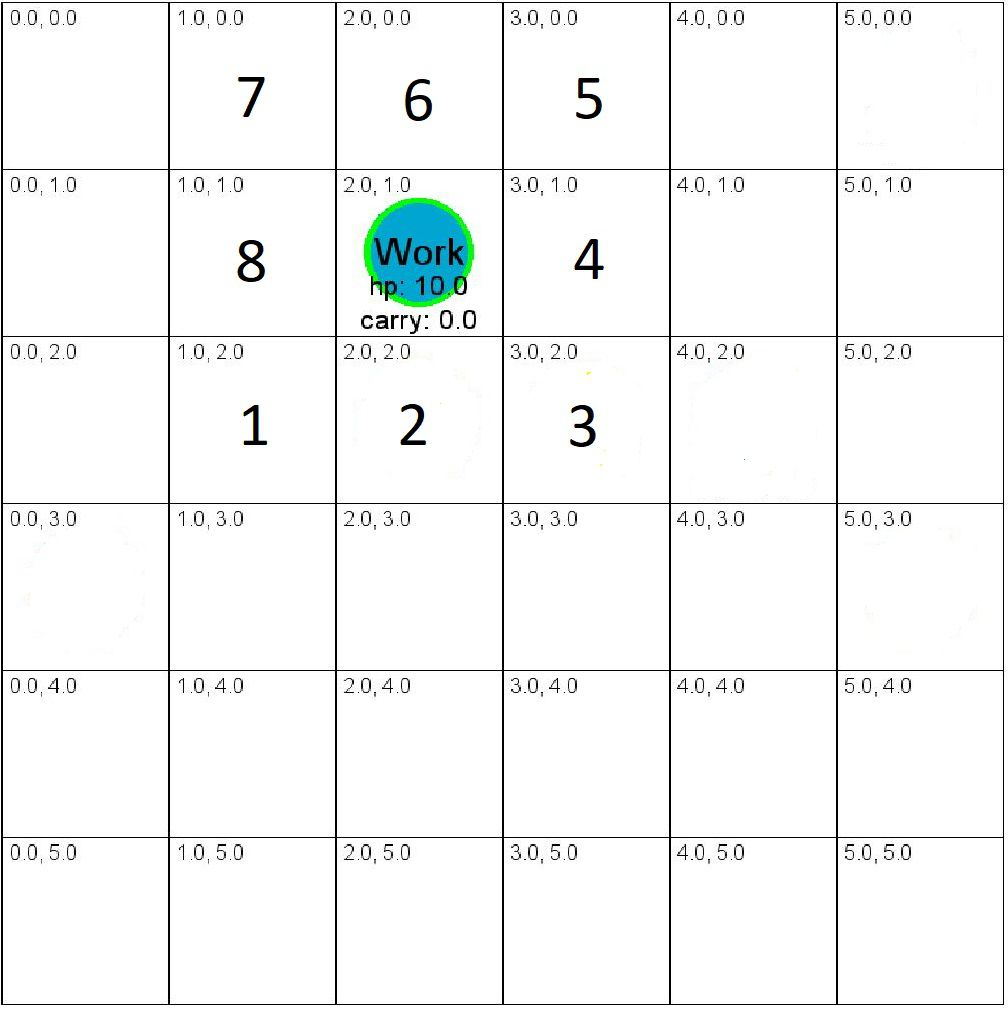
\includegraphics[width=0.6\textwidth]{photos/korakiPreverjanja.pdf}
	\end{center}
	\caption{Na sliki je s številkami označeno zaporedje, v katerem se izvedejo zgoraj navedene akcije. 
		Sprva se vzpostavijo sosednje koordinate, za tem se po zaporedju od prve do zadnje koordinate preverja veljavnost polj. 
		Ko je doseženo prvo veljavno polje, se izbere to polje kot primerno. }
	\label{pickorakiPreverjanja}
\end{figure}

\noindent
Ko je doseženo prvo prazno polje v tem zaporedju, se tam izgradi nova stavba ali izuri nova figura.
Ko je izbrana prva nasprotnikova figura v tem zaporedju, je napadena.
Rezultat tega je gradnja stavb in urjenje figur v spodnji levi kot šahovnice, saj so izbrana prva polja v zaporedju, kot na primer x~-~1, y~+~1, in širjenje proti zgornjim desnim kotom, ko so vsa ostala polja zasedena oziroma tam ni nasprotnikovih figur.

Algoritem smo popravili tako, da smo spremenili te akcije (razen naberi zlatnike in vrni zlatnike), da so posamezne akcije za vsako izmed štirih sosednjih polj.
Za vpeljavo posameznih akcij smo se odločili, ker ne moramo izbrati polja po zgornjem zaporedju tako, da bi bilo za oba igralca enako.\\

\section{Kodiranje}
\label{kodiranja}
\begin{table}
	\begin{center}
	\begin{tabular}{p{0.15\linewidth}|p{0.3\linewidth}|p{0.18\linewidth}|p{0.17\linewidth}}
		Ime figure          & {\tt Akcije}                                                              & {\tt Življenjske točke} & {\tt Strošek izdelave} \\ \hline
		{\tt polje zlata}   & /                                                                         & 10            & 0 \\
		{\tt delavec}       & smeri premikanja, vojašnica, glavna hiša, naberi in vrni zlatnike, zdravi & 10            & 1 \\
		{\tt vojašnica}     & vojak, zdravi                                                             & 10            & 4 \\
		{\tt vojak}         & smeri premikanja, napad, zdravi                                           & 20            & 2 \\
		{\tt glavna hiša}   & delavec, zdravi                                                           & 30            & 7 \\
	\end{tabular}
	\end{center}
	\caption{Tu so opisane figure z njihovimi akcijami in nastavljenimi atributi.}
	\label{tabelfigures}
\end{table}

Določili smo začetno stanje vsake igre, kjer sta glavni hiši igralcev postavljeni v sredino mreže, zraven njiju pa ima vsak igralec svoje polje zlata. 
Vsakemu igralcu se na začetku doda določena količina denarja za izgradnjo začetnih delavcev. 
V našem primeru je bilo to 1, tako da je lahko izgradil samo enega delavca.

Sedaj smo morali zakodirati to stanje igre v numerični prikaz, ki ga bo nevronska mreža lahko interpretirala. 
To stanje lahko zakodiramo z desetiškim kodiranjem, vendar obstaja možnost, da nevronska mreža sloni proti boljšim obravnavanjem pozitivnih števil za igralca +1, kot za igralca -1. 
Ravno iz tega razloga obstaja kodiranje z enico v zapisu vsakega stanja (ang. one-hot encoding; 1-od-N), ki spremeni desetiška števila v binarni vektor (glej Tabelo ~\ref{oneHotEncoder}).

Akciji naberi in vrni zlatnike ostaneta še vedno po 1 akcija, ker za figuro delavec ni razlike, iz katerega sosednjega polja zlata vzame zlatnike, kot tudi ni razlike pri njihovem vračanju.

\subsection{Desetiško}
Pri desetiškim kodiranju, predstavimo vsak atribut figure z eno desetiško številko.
Ker imamo figure s 6 atributi, lahko stanje zakodirane igre predstavimo z dimenzijami širina x višina x 6.
Igralec predstavlja številko -1 za igralca -1, 1 za igralca 1 in 0 za prazno polje.

\subsection{Kodiranje z enicami v zapisu}
\label{oneHotEncoder}
\begin{table}
	\begin{center}
		\begin{tabular}{p{0.19\linewidth}|p{0.13\linewidth}|p{0.58\linewidth}}
			Ime kodirnega polja                        & {\tt št kodirnih bitov} & {\tt Opis} \\ \hline
			{\tt ime igralca}                          & 2                       & Figura na polju je lahko predstavljena z 2 bitoma zaradi treh različnih možnosti: 00 predstavlja prazno polje, 01 predstavlja igralca 1 in 10 igralca -1.\\
			{\tt tip figure}                           & 3                       & Predstaviti moramo 5 različnih figur, kar lahko zakodiramo z najmanj 3 biti.\\
			{\tt število življenjskih točk}            & 5                       & Nekatere figure imajo veliko življenjskih točk (npr. glavna hiša 30), za kar moramo uporabiti 5 bitov. 
																                   Uporabili smo večje število življenjskih točk, tako da lahko uspešno deluje oslabitvena funkcija (Slika~\ref{destroy_formula_2018_11_17}), da se število življenjskih točk figuram ne zmanjša prehitro.\\
			{\tt nosi zlatnike}                        & 1                       & Zastavica, ki se postavi na 1, ko figura delavec nosi zlatnike, drugače je postavljena na 0.\\
			{\tt denar}                                & 5                       & Za ta kodirnik smo uporabili večje število, saj pustimo, da igralec gradi ekonomijo in shranjuje denar, da ga potem lahko na hitro zapravi na figurah, ko ga ima dovolj za njihovo izgradnjo.
																                   To lahko privede v zanimive taktike hranjenja denarja in za tem hitro izgradnjo vojaških enot za napad nasprotnikovih figur.\\
			{\tt čas igranja}                          & 11                      & Atribut, predstavljen z 11 biti ($2^{11}$ = 2048), ki dovoljuje igralcu dovolj časa, da odkriva nove poteze, ampak ga dovolj hitro omeji, da se igra konča in začne nova.\\
		\end{tabular}
	\end{center}
	\caption{Predstavitev števila kodirnih atributov za posamezni kodirnik in pojasnitev odločitve za število kodirnih bitov. }
	\label{tableEncodersOneHot}
\end{table}

Dimenzija zakodiranega prostora je tako širina x višina x 22, kar je 3.6-krat število, ki kodira posamezno stanje igre z desetiškim kodirnikom.
To zna otežiti učenje nevronske mreže, ker se s tem kodiranjem poveča velikost izhodnega vektorja $Pi$, ki predstavlja napoved posamezne akcije.

\section{Konec igre}
\label{sKonecIgre}
Konec igre se izvede pod določenimi pogoji:
\begin{itemize}
	\item igralec nima za izvesti več nobene možne akcije,
	\item vse figure igralca so uničene,
	\item ko se izteče čas.
\end{itemize}
\noindent
Zaradi primera, kjer se igra nikoli ne zaključi, saj se na primer delavci premikajo v ciklu in se tako igra nikoli ne konča, smo morali določiti umeten konec igre.
S tem smo odstranili neskončne cikle igranja igre in prisilili igralca k hitrejšemu izvajanju akcij.

\subsection{Oslabitvena funkcija}
\label{sKillFunction}
Čakanje, da se čas igre izteče je problematično, saj učenje modela poteka zelo počasi, posebej ko algoritem MCTS raziskuje preiskovalni prostor akcij.
Za to smo razvili funkcijo, ki prisili model k izvajanju akcij v zgodnjem času igre, drugače se figuram preveč začnejo zmanjševati življenjske točne in so zato odstranjene s šahovnice.
Figure lahko uporabijo akcijo zdravljenja, s čimer povečajo trenutno število življenjskih točk določene figure največ do njene zgornje meje.

\begin{figure}[h!]
	\begin{center}
		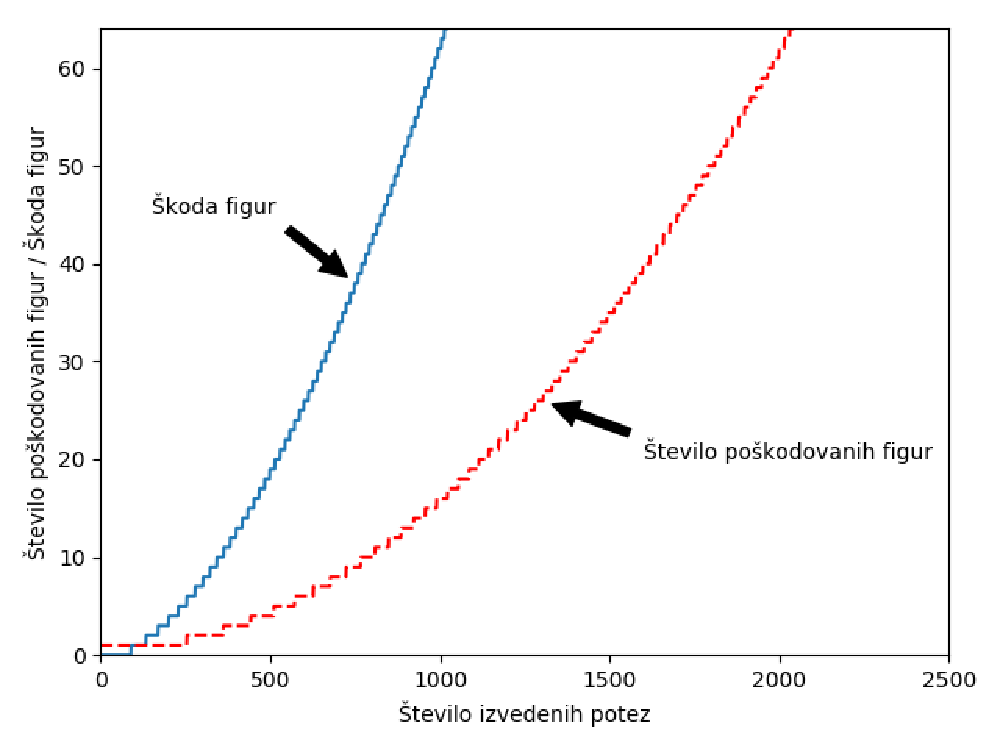
\includegraphics[width=0.8\textwidth]{photos/destroy_formula_2018_11_17.pdf}
	\end{center}
	\caption{Na grafu sta narisani dve funkciji, ki določata zmanjšanje življenjskih točk, kar se obravnava v določeni figuri v danem času igre~(modra) in pri tem se upošteva koliko igralcev je bilo poškodovanih v trenutnem časovnem okviru~(rdeča).
	Vidimo, da je krivulja zmanjšanja življenjskih točk veliko bolj stroga in se v igri začenja že zelo zgodaj. 
	To je zato, ker želimo hitro odpraviti nedejavne igralce in tiste, ki zbirajo zlatnike in pridobivajo nove figure.
	Vidimo tudi y-osi od 0 do 64, kar je največje število igralcev za enega igralca, tako da bo pri približno 2000 korakih vsaka figura dobila smrtno poškodbo, zato časovni potek nikoli ni dosežen.}
	\label{destroy_formula_2018_11_17}
\end{figure}

Z oslabitveno funkcijo je bil problem določiti pravo stopnjo količine zman- jšanja življenjskih točk figur in izločevanje neaktivnih igralcev dovolj zgodaj v igri, in sicer je bil problem z uravnovešanjem količine in stroškom zdravljenja. 
Če so bili stroški dovolj nizki, so igralci stalno zdravili figure in končali igro z vedno več izvedenimi potezami (npr. tisoč), kar je privedlo do vedno daljših iger in daljšega postopka igranja.
Za to je bilo potrebno povišati strošek zdravljenja, kar je privedlo do hitrejšega nenadnega izločevanja figur, saj igralci niso imeli dovolj zlatnikov za zdravljenje, na kar je bilo potrebno povišati količino vrnjenih zlatnikov iz figure zlata.

\subsection{Ustavitveni pogoj}
Ustavitveni pogoj deluje tako, da se na številu določenih potez igra preprosto prekine in oceni zmagovalca po eni izmed spodaj navedenih formul.
Igra se prekine po 100-200 potezah, če si do takrat igralca med sabo nista uničila figur.
V spodnjih treh izrekih sta igralec 1 in 2 označena s p1 in p2.

\begin{izrek}
	\label{ustavitvenipogoj1}
Prvi: igralec 1 zmaga, če ima več denarja kot igralec 2.
	\begin{equation}
p1.zlatniki > p2.zlatniki
	\label{eq:ustavitvenipogoj1}
	\end{equation}
\end{izrek}
\noindent
Prvi izrek je dober ustavitveni pogoj za testiranje igralcev pri nabiranju zlatnikov, kjer zmaga preprosto tisti, ki jih nabere več.

\begin{izrek}
	\label{ustavitvenipogoj2}
Drugi: igralec 1 zmaga, ko je seštevek zdravja vseh figur igralca 1 večje od seštevka zdravja vseh figur igralca 2.
	\begin{equation}
	\sum{p1.figure.zdravje} > \sum{p2.figure.zdravje}
	\label{eq:ustavitvenipogoj2}
	\end{equation}
\end{izrek}
\noindent
Če je pogoj za zmago večje število življenja svojih figur kakor nasprotnikovih, hkrati pomeni, da lahko igralec nabira več zlatnikov in z njimi gradi nove stavbe in uri nove enote, kar zagotavlja za igralca večjo skupno vsoto življenja figur in hkrati zagotavlja težnjo k urjenju vojaških enot z namenom, da nasprotnikovim enotam zmanjša število življenjskih točk.

\begin{izrek}
	\label{ustavitvenipogoj3}
Tretji: igralec 1 zmaga, ko je seštevek zdravja vseh figur igralca 1 plus njegov denar večje od seštevka zdravja vseh figur igralca 2 plus njegov denar.
	\begin{equation}
	\sum{p1.figure.zdravje} + p1.zlatniki > \sum{p2.figure.zdravje} + p2.zlatniki
	\label{eq:ustavitvenipogoj3}
	\end{equation}
\end{izrek}
\noindent
K drugemu izreku smo dodali trenutno število shranjenih zlatnikov igralca, kar dodatno spodbudi motivacijo igralca k nabiranju novih zlatnikov.
V večini učnih primerov, kot smo to opisali v poglavju~\ref{chrezultati}, smo uporabljali tretji ustavitveni pogoj~\ref{ustavitvenipogoj3}, saj združuje tako življenjske točke enot kot tudi denar.
Vendar imajo figure običajno veliko več življenjskih točk kolikor so vredne, tako da je izgradnja nove figure za igralca primernejša, kot da bi denar shranjeval.

%%%%%%%%%%%%%%%%%%%%%%%%%%%%%%%%%%%%%%%%%%%%%%%%%%%%%%%%%%%%%%%%%%%%%%%%%%%%%%%%%%%%%%%%%%%%%%%%%%%%%%%%%%%%%%%%%%%%%%%%
%%%%%%%%%%%%%%%%%%%%%%%%%%%%%%%%%%%%%%%%%%%%%%%%%%%%%%%%%%%%%%%%%%%%%%%%%%%%%%%%%%%%%%%%%%%%%%%%%%%%%%%%%%%%%%%%%%%%%%%%
%%%%%%%%%%%%%%%%%%%%%%%%%%%%%%%%%%%%%%%%%%%%%%%%%%%%%%%%%%%%%%%%%%%%%%%%%%%%%%%%%%%%%%%%%%%%%%%%%%%%%%%%%%%%%%%%%%%%%%%%
%%%%%%%%%%%%%%%%%%%%%%%%%%%%%%%%%%%%%%%%%%%%%%%%%%%%%%%%%%%%%%%%%%%%%%%%%%%%%%%%%%%%%%%%%%%%%%%%%%%%%%%%%%%%%%%%%%%%%%%%
%%%%%%%%%%%%%%%%%%%%%%%%%%%%%%%%%%%%%%%%%%%%%%%%%%%%%%%%%%%%%%%%%%%%%%%%%%%%%%%%%%%%%%%%%%%%%%%%%%%%%%%%%%%%%%%%%%%%%%%%

\chapter{Učenje modela}
\label{chucenjemodela}
Ena izmed glavnih komponent učnega postopka je seveda nevronska mreža, ki hrani moči povezav določenih akcij ob določenem stanju igre.
V tem poglavju bomo sprva predstavili zgradbo nevronske mreže s tehničnega vidika, nato se bomo posvetili predstavitvi parametrov, ki so nastavljivi pri postopku učenja.
Od njih je odvisno, koliko časa in na kakšen način se bo naš model učil ob nastavljeni konfiguraciji igre.
Na koncu poglavja se bomo poglobili v možno tehniko postopnega učenja modela, kjer postopno dodajamo zahtevnejše konfiguracije in pravila igre.

\section{Zgradba nevronske mreže}
Implementirali smo štiri vrste igralcev, ki lahko igrajo strateško igro.
Prva vrsta je človeški igralec, za katerega smo morali implementirati uporabniški vmesnik, preko katerega izvršuje akcije na prikazani šahovnici.
Druga je naključni igralec, ki naključno izvaja akcije, ki so v trenutnem stanju igre možne.
Njegova izboljšava je igralec, ki temelji na požrešni metodi.
Ta stremi k čim hitrejšemu povečanju točk, ki temeljijo na enem izmed ustavitvenih pogojev.
O četrti implementaciji igralca pa govori jedro diplomske naloge, in sicer ga predstavlja nevronska mreža z naučenimi utežmi.

Za implementacijo nevronske mreže smo uporabili modul Keras znotraj knjižnice TensorFlow.
Programska koda za izgradnjo modela je lažje berljiva v modulu Keras kakor v TensorFlow, zato smo se zanj tudi odločili.
Ker je modul Keras od verzije 1.9, izdane leta 2017, impementiran znotraj knjižnice TensorFlow, ni bilo večjih težav z njeno namestitvijo na odjemalčevem računalniku z vtičnikom TensorFlow-UE4~\cite{ue4tf}.

Model za vhod vzame učne množice stanja iger dimenzij širina x višina x število kodirnikov, kar je v primeru numeričnega kodirnika 8 x 8 x 6 in v primeru kodirnika 1-od-N 8 x 8 x 30.
Potem gre ta učna množica skozi 4 konvolucijske nivoje, kjer je velikost filtra 3 in ima nastavljivo globino, ki je v našem primeru 128.
Prva dva konvolucijska nivoja imata oblogo ničel okrog matrike, tako da se velikost nivoja ne zmanjša, druga dva te obloge nimata, kar zniža velikost nivoja z 8 x 8 na 4 x 4, tako da je izhod zadnjega konvolucijskega nivoja dimenzije velikost serije x (širina - 4) x (višina - 4) x število kanalov.

Vsak izhod konvolucijskih nivojev s postopkom normalizacije serije (ang. batch normalization) normalizira aktivacijo prejšnjega nivoja ob vsaki seriji.
Izhodi tega se preuredijo z relu aktivacijsko funkcijo, ki za vsa negativna števila vzame vrednost 0.
Za tem se izhod zadnjega nivoja normalizirane konvolucije izravna v 1-dimenzionalni vektor in se poda dvema polno povezanima nivojema, ki sta ponovno normalizirana z normalizacijo serije.
Ta dva nivoja sta potem ponovno preoblikovana z relu aktivacijsko funkcijo in podana v izpadno funkcijo (ang. dropout), ki prepreči prekomerno prileganje.

Za tem je izgrajen polno povezan nivo $Pi$, ki ima tolikšno število izhodov, kolikor je možno število akcij v igri za vsako celico, ki ima aktivacijsko funkcijo softmax.
Izgrajen je tudi polno povezan nivo $V$, ki ima en izhod, ki predstavlja zmago ali poraz s tanh aktivacijsko funkcijo.
Za izhod $Pi$ se nastavi funkcija izgube kategorična prečna entropija, in MSE za izhod $V$.

\begin{figure}[h!]
	\begin{center}
		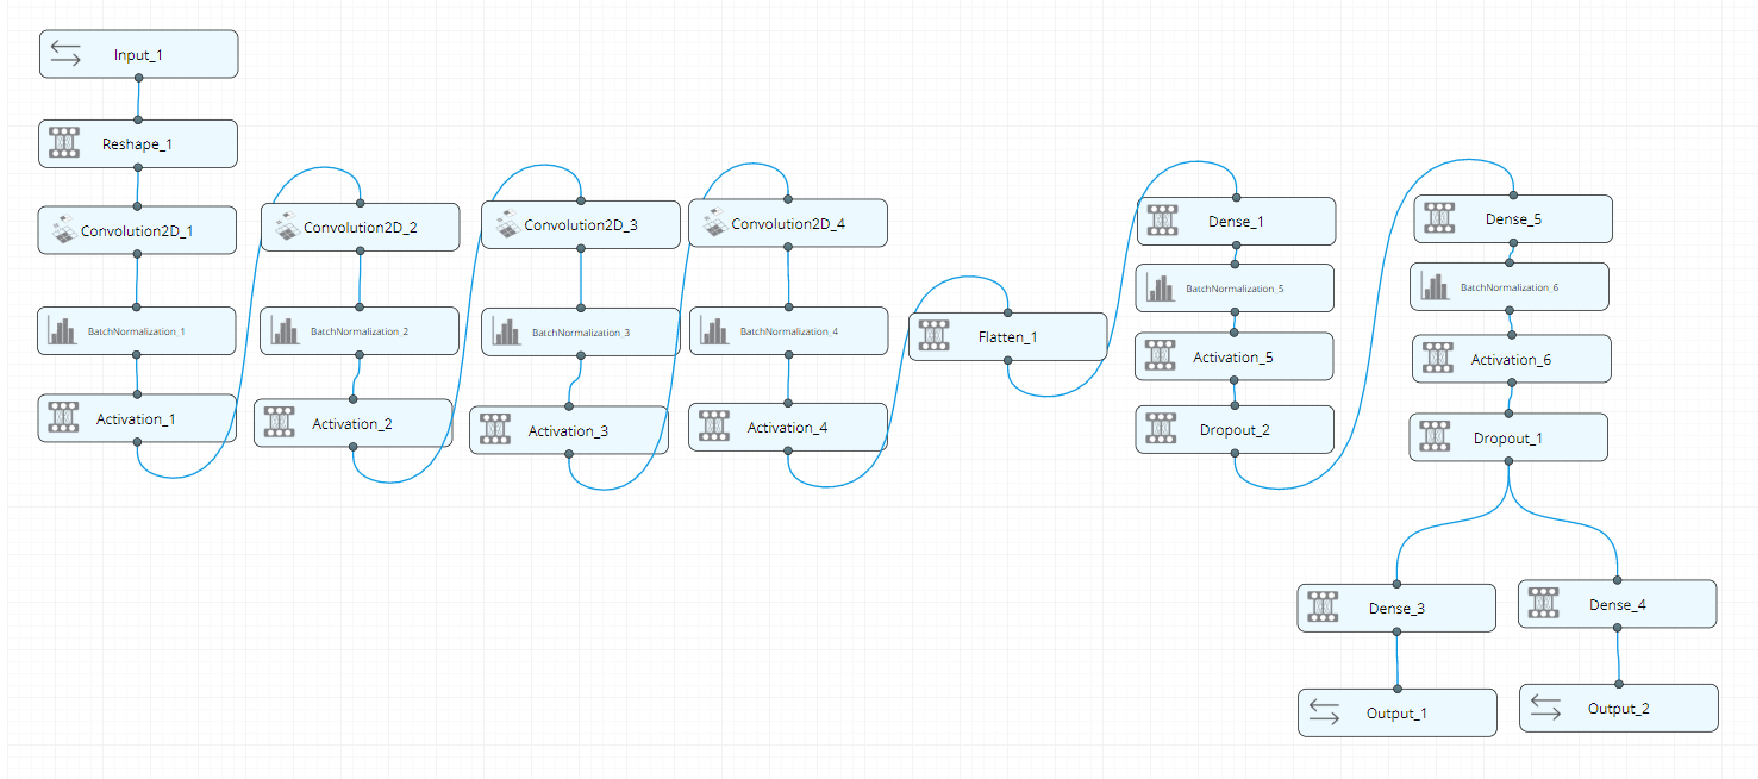
\includegraphics[width=0.55\textwidth]{photos/model_using_deepcognition.pdf}
	\end{center}
	\caption{Model nevronske mreže, uporabljen za učenje igre. Izgrajen je iz štirih konvolucijskih nivojev, med katerimi je izhod normaliziran in preoblikovan z relu aktivacijsko funkcijo. 
		Nato se poda izhod zadnjega konvolucijskega nivoja v dva polno povezana nivoja, za katerima se določi izhod $V$ in $Pi$, ki predstavljata napoved zmage (V) in napovedi verjetnosti akcij (Pi).
		Slika je bila izdelana z uporabo aplikacije Deep Learning Studio~\cite{deepcognition}.}
	\label{vizualzacijaModela}
\end{figure}

\section{Predstavitev parametrov}
\label{parametri}
Učni algoritem uporablja množico parametrov za učenje, ki zelo vplivajo na hitrost in moč učenja.
Ti predstavljajo različno število iteracij igranja iger (iteracije in epizode igranja), kot tudi iteracij učenja nevronske mreže oziroma število epoh (ang. epoch).
Predstavljajo tudi same nastavitve raziskovanja algoritma MCTS (C\textsubscript{p,uct}) in število primerjav, kateri naučen model je boljši.

V tabeli opisa parametrov~\ref{tableParameters1} so predstavljeni najpomembnejši parametri, ki smo jih spreminjali ob učenju modela na naši RTS igri.
\begin{table}
	\begin{center}
		\begin{tabular}{p{0.15\linewidth}|p{0.13\linewidth}|p{0.62\linewidth}}
			Ime parametra                             & {\tt Privzeta vrednost} & {\tt Opis} \\ \hline
			{\tt C\textsubscript{p,uct}}               & 1 						& Parameter drevesnega raziskovanja, ki neposredno vpliva na raziskovanje algoritma MCTS. 
																				  Večja kot je vrednost parametra, bolj bo MCTS dajal prednost neraziskanim vozliščem. 
																				  V našem primeru smo izbrali vrednost 1 in s tem nismo prispevali k dodatni uteži k raziskovanju.\\
			{\tt število iteracij}                    & 30-100				    & Predstavlja število učenj algoritma na odigranih igrah in število izbir boljšega modela.
																				  Parameter tudi predstavlja, kolikokrat se bo igra odigrala v celoti, kjer bo konec predstavljal končni pogoj oziroma poraz nasprotnika.\\
			{\tt število epizod}                      & 4-8 					& Število epizod nam zagotovi pridobitev dovolj velikega nabora odigranih iger, nad katerimi se potem model uči.
																				  Ta parameter določa število ponovitev iger ob vsaki iteraciji.\\
			{\tt število MCTS iskanj}                 & 30-50					& Predstavlja število raziskanih vozlišč v iteraciji igre. 
														 						  MCTS iskanja se ne izvršijo do konca igre, ampak do neraziskanega vozlišča ali če je raziskano vozlišče konec igre~\cite{silver2018general}.
														 						  Bodimo pozorni na majhno število MCTS iskanj (30-50), za razliko od tradicionalnih algoritmov MCTS, ki na primer v igri šah odigrajo več desettisoč iteracij~\cite{kohne}.\\ 
		\end{tabular}
	\end{center}
	\label{tableParameters1}
\end{table}

\begin{table}
	\begin{center}
		\begin{tabular}{p{0.16\linewidth}|p{0.13\linewidth}|p{0.61\linewidth}}

			{\tt število primerjanj modelov}  		  & 10 						& Pove, olikokrat se bosta trenutni model, ki se uči, in njegova prejšna različica pomerila med sabo, da se ohrani boljši.
																				  Naučena modela se med sabo pomerita z igranjem iger od začetka do konca, kjer je rezultat zmaga nekoga izmed modelov oziroma neodločeno.\\
			{\tt število iteracij učnih primerov}     & 8 						& Zagotavlja nam, da ohranjamo novejše učne primere in starejše zavržemo.
																				  Vsako epizodo se doda nova zbirka iger ter odstrani najstarejša, če število shranjenih epizod presega ta parameter.
																				  To nam zagotavlja dovolj svežo učno množico, nad katero se nevronska mreža uči.
																				  V našem primeru je bil nastavljen na manjšo vrednost (8), saj kodiranja stanj naše igre zasedejo veliko pomnilnika.\\
			{\tt število epoh}     					  & 30-100 				    & Število iteracij učenja nevronske mreže skozi učne primere.\\
		\end{tabular}
	\end{center}
	\caption{Opis najpomembnejših učnih parametrov, uporabljenih pri učenju algoritma AlphaZero. Pri parametrih so zapisana tudi njihova okvirna oziroma največkrat uporabljena konfiguracijska števila.}
	\label{tableParameters2}
\end{table}

\section{Postopno učenje}
Učenje te igre je zapleteno zaradi pogojev konca igre. 
Algoritem izvaja igranje igre, dokler ne doleti do ustavitvenega pogoja.
Ta pri RTS igri lahko ni nikoli dosežen, saj se lahko vojaška enota stalno premika v istem krogu, kakor bi se lahko trdnjava vedno premikala samo po dveh istih poljih.
Cikel akcij se lahko reši z uporabo časovnih omejitev, kjer se igranje igre ustavi, ko se izteče čas, vendar to povzroča bolj površen približek ocene stanja igre, ki vpliva na učenje nevronske mreže.
Zaradi kompleksnejšega ustavitvenega pogoja se lahko model hitro prekomerno prilagodi na napačno igranje igre.
Dober primer je ustavitveni pogoj z vsoto zdravja igralčevih enot in njegovih trenutnih zlatnikov (Izrek~\ref{eq:ustavitvenipogoj3}), kjer se igralca ne naučita pravilno napadati nasprotnikovih enot, da znižujeta nasprotnikove življenjske točke, ampak konstantno nabirata nove zlatnike in gradita in urita nove enote, ker igralca nista naučena, kako zaključiti igro z uničevanjem nasprotnikovih enot.

Iz tega razloga se nam je porodila učna ideja s postopnim učenjem modela. 
Ideja govori o spreminjanju pravil iger in nastavitev parametrov med učenjem.
S tem bi lahko v začetnih fazah učenja dali prednost nabiranju zlatnikov in s tem naučili algoritem uspešnega in hitrega nabiranja kot ustavitveni pogoj 1 (Izrek~\ref{eq:ustavitvenipogoj1}).
Za tem bi ta naučeni model nadgradili na tak način, da bi mu spremenili ustavitveni pogoj na 2 (Izrek~\ref{eq:ustavitvenipogoj2}) in h konfiguraciji akcij dodali možnost gradnje stavb, s čimer bi zdajšnji model, ki dobro nabira zlatnike, z nadaljnjim učenjem nadgradili, da bi poleg nabiranja gradil hiše in s tem povečeval število življenjskih točk enot, ki jih igralec obvladuje.
Ta model bi v tretji fazi nadgradili z akcijami urjenja vojaških enot in napadom drugega igralca.

Poskusili smo naučiti model po zgoraj opisanem postopku, vendar učenje ni potekalo uspešno.
Nevronska mreža je vzpostavila začetna stanja vrednosti vozlišč akcij po vnaprej naučenih utežeh, pridobljenih iz naučenega modela, ki v fazi 2 ali 3 ni vseboval novo dodanih akcij, kot so gradnja stavb oziroma napadanje.
Zaradi majhnega ocenjenega stanja novih akcij so te manjkrat obiskane in zato manj raziskane.
Algoritem zaradi sprememb pravil igre deluje zelo naključno, saj naučene uteži delujejo v nasprotju z igralčevimi željami.
MCTS pri tem iskanju ne pripomore veliko, saj so neraziskana stanja igre vzpostavljena glede na uteži iz nevronske mreže.
Stanje se popravi, ko doseže končno stanje, kar se zgodi redko.

%%%%%%%%%%%%%%%%%%%%%%%%%%%%%%%%%%%%%%%%%%%%%%%%%%%%%%%%%%%%%%%%%%%%%%%%%%%%%%%%%%%%%%%%%%%%%%%%%%%%%%%%%%%%%%%%%%%%%%%%
%%%%%%%%%%%%%%%%%%%%%%%%%%%%%%%%%%%%%%%%%%%%%%%%%%%%%%%%%%%%%%%%%%%%%%%%%%%%%%%%%%%%%%%%%%%%%%%%%%%%%%%%%%%%%%%%%%%%%%%%
%%%%%%%%%%%%%%%%%%%%%%%%%%%%%%%%%%%%%%%%%%%%%%%%%%%%%%%%%%%%%%%%%%%%%%%%%%%%%%%%%%%%%%%%%%%%%%%%%%%%%%%%%%%%%%%%%%%%%%%%
%%%%%%%%%%%%%%%%%%%%%%%%%%%%%%%%%%%%%%%%%%%%%%%%%%%%%%%%%%%%%%%%%%%%%%%%%%%%%%%%%%%%%%%%%%%%%%%%%%%%%%%%%%%%%%%%%%%%%%%%
%%%%%%%%%%%%%%%%%%%%%%%%%%%%%%%%%%%%%%%%%%%%%%%%%%%%%%%%%%%%%%%%%%%%%%%%%%%%%%%%%%%%%%%%%%%%%%%%%%%%%%%%%%%%%%%%%%%%%%%%

\chapter{Vizualizacije}
\label{chvizualizacija}

\section{Pygame}
S Python knjižnico Pygame smo izdelali vizualizacijo, ki je primerna za pregled igre med samim razvijanjem. 
Šahovnica je označena s črtami, med katerimi so s krogi izrisane figure, kjer njihove barve predstavljajo svoj tip figure in obroba krogca igralca -1 ali +1.
V krogcih je tudi napisano število življenjskih točk za to figuro in zastavica, ali delavec prenaša zlatnike.
Zgoraj je izpisano, koliko denarja ima posamezen igralec in koliko potez sta igralca že odigrala ter vse možne akcije, ki jih igralec lahko izvrši z določeno figuro.

Igralec lahko nadzoruje svoje figure s tipkovnico in miško.
Uporabnik mora najprej izbrati figuro z levim miškinim klikom in potem izbrati določeno akcijo, ki je izpisana na zaslonu. 
Uporabnik lahko spremeni figuro, tako da jo odznači s klikom desnega miškinega gumba na prazno mesto.

\begin{itemize}
	\item premikanje: Igralec lahko premakne delavce in vojake za 1 kvadratek v vseh 4 smereh, če so prazni, s klikom na eno od 4 mest.
	\item napadanje: Z izbrano vojaško figuro lahko uporabnik napade nasprotnikove figure, ki so v dosegu.
	\item zbiranje in vračanje sredstev: Z izbranim delavcem lahko uporabnik nabere zlatnike, tako da klikne z desno miškino tipko na polje zlata, če je v dosegu polja zlata.
	Podobno lahko stori za vračanje zlatnikov, kjer pa mora z izbranim delavcem, ki nosi zlatnike in je v bližini glavne hiše, klikniti na glavno hišo, na kar delavec vrne zlatnike igralcu.
	\item gradnja: Za gradbene figure in zgradbe mora uporabnik uporabiti eno od bližnjic na tipkovnici.
\end{itemize}
\noindent
Igralec lahko igro igra tudi s pisanjem akcij v Python konzolo.

\begin{figure}[h!]
	\begin{center}
		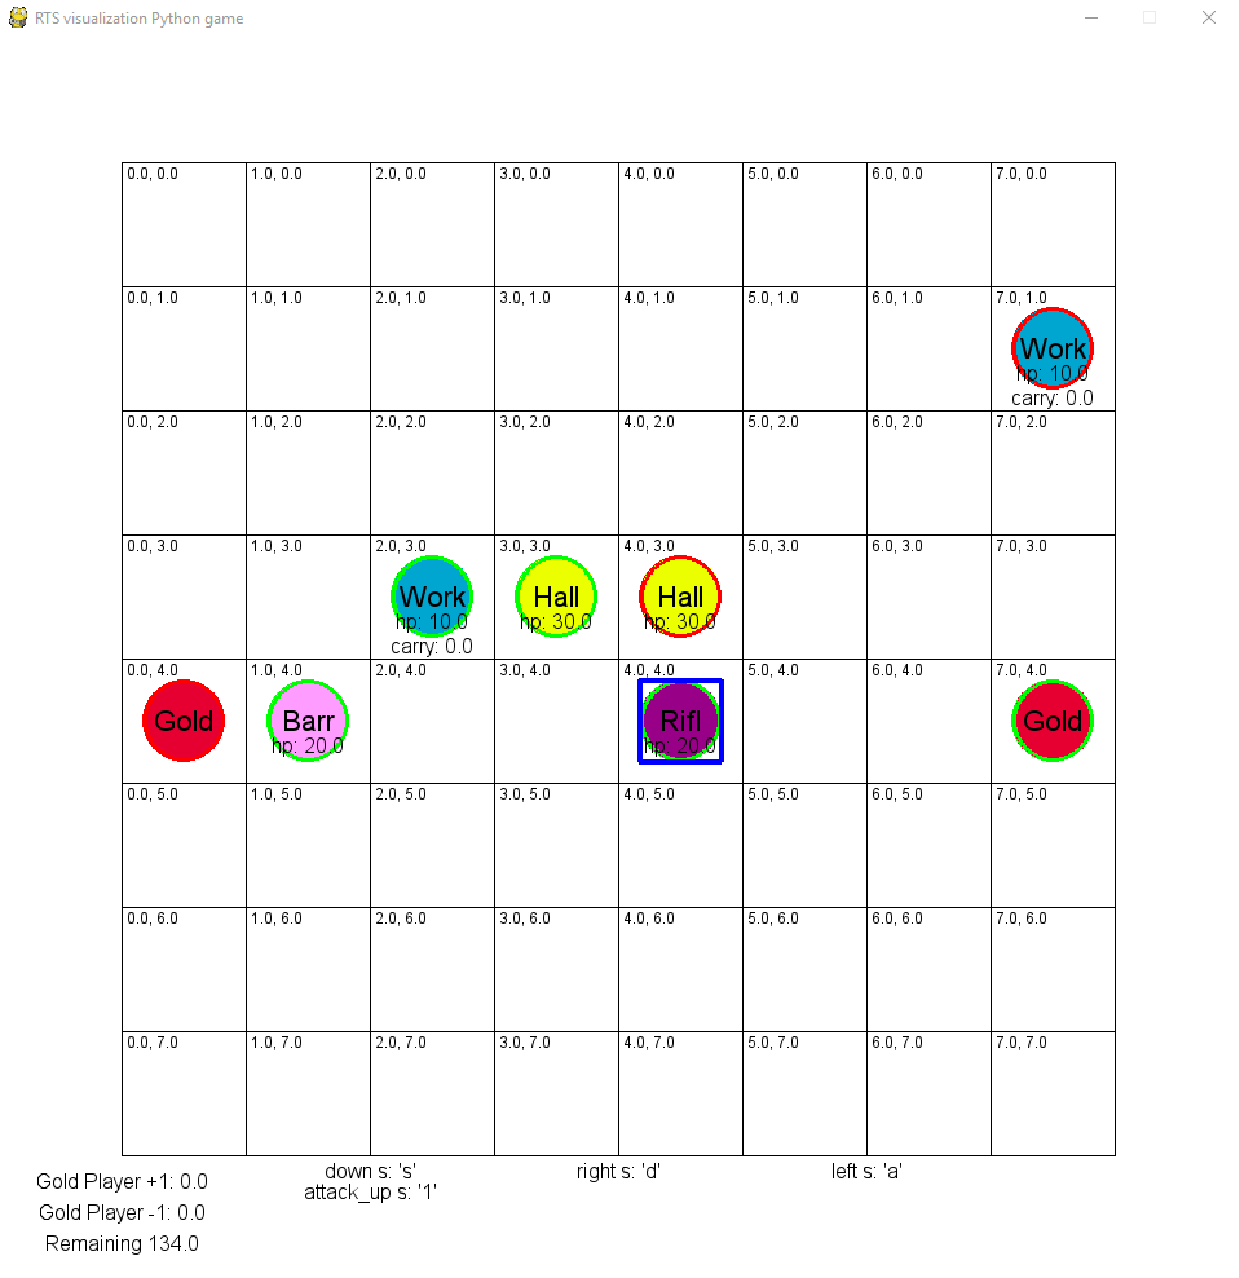
\includegraphics[width=0.9\textwidth]{photos/visualization_pygame.pdf}
	\end{center}
	\caption{Na zgornji sliki človeški igralec igra izgrajeno strateško igro proti računalniškim nasprotnikom.}
	\label{visualization_pygame}
\end{figure}

\section{Unreal Engine 4}
\label{UnrealEngine}

Celostni pogon Unreal Engine 4 (ang. game engine Unreal Engine 4; UE4) je odprto-kodni program podjetja Epic Games, ki je namenjen hitri izdelavi računalniških iger. 
Obstajajo drugi celostni pogoni, kot je na primer Unity.\\
Unreal Engine 4, ki omogoča hitro ustvarjanje iger s pomočjo posebnih diagramov (ang. blueprint) in hkrati podpira programski jezik C++, ki ga uporabimo za hitro izvedbo velikega števila matematičnih izrazov~\cite{diploma2}.

\begin{figure}[h!]
	\begin{center}
		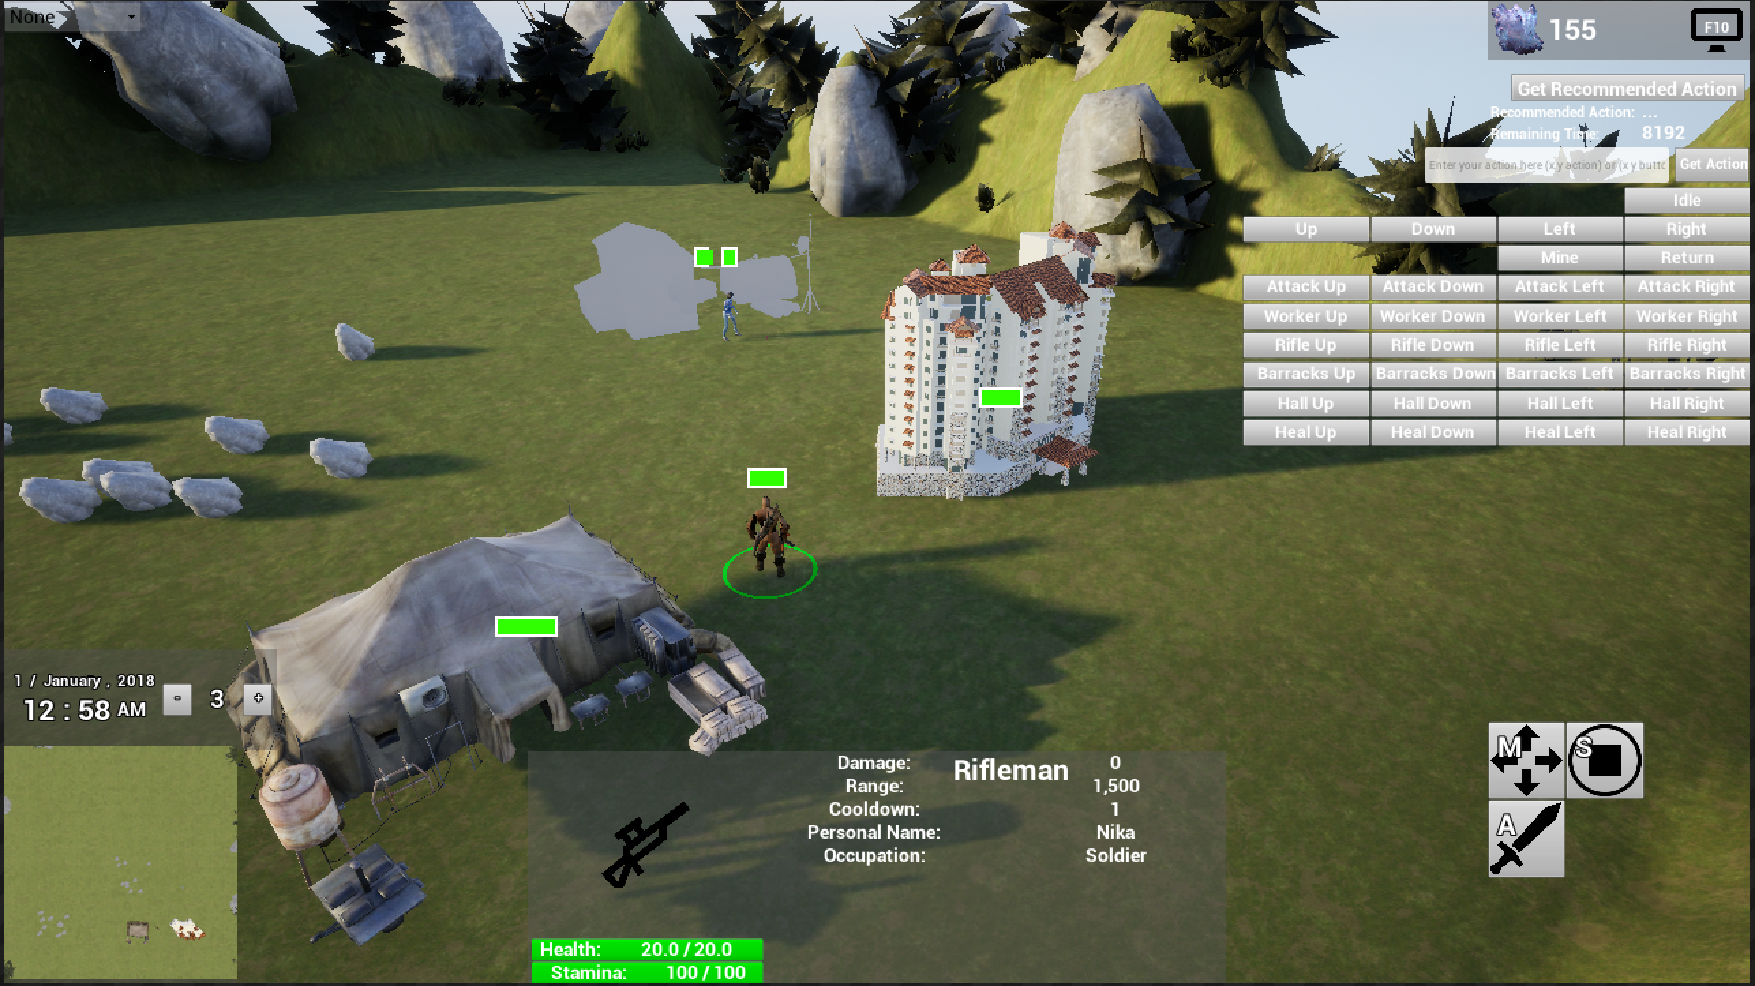
\includegraphics[width=0.8\textwidth]{photos/ue4-widget.pdf}
	\end{center}
	\caption{Zgornja slika predstavlja igro, izdelano v Unreal Engine 4 z uporabniškim vmesnikom. 
		Na sliki so vidni glavna hiša, vojašnica, vojak in delavec ter polje zlata na levi. 
		Igralec lahko upravlja z vmesnikom za pošiljanje prošenj, s katerimi predlaga poteze in je nakazan v vnosnem polju in z gumbi na desni strani slike.}
	\label{ue4-game}
\end{figure}

V temu programu smo oblikovali vizualizacijo igre, ki nam je omogočila bolj moderen in realističen prikaz realno-časovne strateške igre, saj je vizualizirana v 3-D in ne 2-D kot v Pygame.

V igri lahko izvajamo akcije preko uporabniškega vmesnika kot tudi z bližnjicami na tipkovnici.
Kompleksnejši uporabniški vmesnik nam zagotavlja več funkcionalnosti kakor igra, izdelana v Pygame.
Z njim lahko izbiramo več figur ter jih združujemo v skupine.
Figuram postavljamo več zaporednih akcij, ki jih ta izvršuje v tem vrstnem redu.
Človeški igralec ima tudi vpogled na manjši zemljevid, prikazan v levem spodnjem kotu, na katerem vidi nasprotnikove in svoje figure.
Nekaj je tudi kozmetičnih funkcij, kot so npr. prekrivanje zemljevida z meglo (ang. fog of war), dnevno-nočni cikel, animacije za vojskovanje, premikanje, nastavitve hitrosti časa ipd.

Igra ima tudi implementirana izvajalna drevesa, kjer na primer agentu naročimo nabiranje zlatnikov in ta jih sam vrača na najbližje odlagališče zlatnikov.
Izvajalna drevesa so implementirana tudi za napadanje, agentovo nedejavnost, kjer se agent prosto premika okrog, išče stavbe itd.
Igra ima implementirane tudi razne zvočne efekte, učinke delcev za prikaz zmanjšanja življenjskih točk nasprotnikovim enotam.
Stanje igre lahko shranimo na disk in ga pozneje naložimo, da igro lahko igramo naprej.
Ob tem zapisovanju igre smo ugotovili pravi postopek, kako zajeti igro v Unreal Engine in ga zapisati v določen format, ki ga potem lahko lažje prenašamo.
To nam je koristilo tudi pri kodiranju igre v notacijo za označevanje JavaScript objektov (ang. JavaScript Object Notation; JSON), da smo jo lahko poslali Python modula kot parameter v zahtevku.
Igra podpira tudi preprosto analitiko za primerjavo denarja med igralci, tipi figur ipd.

Igra je zasnovana tako, da se lahko dva igralca med sabo pomerita preko mreže s spletnim podsistemom Steam ali preko lokalne mreže, preko katerih lahko tudi komunicirata.
Oba igralca v tem primeru na svojem lokalnem računalniku poganjata naučena modela in od njega zahtevata priporočila akcij.
Ker lahko igralca izbereta več različnih map, na katerih bosta igrala, je potrebno za vsako izmed teh map naučiti svoj model, saj imajo lahko mape drugačne dimenzije v širini in višini.
S sedanjim algoritmom niso pokriti primeri, da določeno polje na šahovnici ni dosegljivo (voda, skalovje), tako da morajo biti mape kvadratne in vsa polja dosegljiva.
Nekatere izmed zgoraj navedenih funkcij je izdelal Nick Pruehs v vtičniku ue4-rts~\cite{rtsUe4}, kot recimo nekatera izvajalna drevesa, zemljevid in prekrivanje zemljevida z meglo.

Akcije in figure je bilo potrebno preslikati v urejevalnik Unreal Engine, da se tam figure primerno premikajo in izvajajo akcije.
To je bilo potrebno storiti tudi za animacije in efekte, da premikanje in napadanje zgleda dokaj realistično.
Ko igralca pričneta z igranjem igre, se naloži TensorFlow model, katerega bosta igralca uporabljala za pridobivanje akcij.
Za lažjo komunikacijo s Python modulom in za vračanje povratnih klicev v celostni pogon smo uporabili vtičnik TensorFlow-UE4~\cite{ue4tf}, ki nadgradi vtičnik UnrealEnginePython~\cite{ue4python} s TensorFlow komponento. 
Ta komponenta se avtomatično naloži na odjemalčevem računalniku in zagotavlja, da lahko ta uporablja vse funkcionalnosti knjižnice TensorFlow.
 
Ko igralec ali računalniški nasprotnik poda zahtevo za pridobitev akcije, se najprej izvede poizvedba o trenutnem stanju igre, ki se jo preslika v JSON zapis, da se ga potem posreduje Python skripti.
V tem JSON zapisu so zapisane figure s kodirniki (x, y, igralec, tip figure, število življenjskih točk, nosi zlatnike, zlatniki, preostali čas).
Potem se JSON zapis asinhrono pošlje Python skripti, da ta izgradi novo šahovnico s figurami na podlagi prejetih zakodiranih figur.
Skripta prejme tudi ime igralca, ki je poslal zahtevek za pridobitev akcije.
Skripta za tem pokliče funkcijo za pridobitev verjetnosti akcij, ki izvede določeno število MCTS iteracij in izbere tisto z največjo verjetnostjo.
Python skripta vrne koordinati x in y ter akcijo, ki se potem izvede v celostnem pogonu s svojimi preslikanimi akcijami za gor, dol, napad, naberi ipd.
Potrebno je bilo tudi paziti z orientacijo koordinatnega sistema, saj je bil v Python igri drugače orientiran kot v pogonu Unreal Engine. 
Potrebno ga je bilo obrniti za -90° v osi Z (pogon Unreal Engine 4: +x~gor, +y~desno, Python igra: +x~desno, +y~dol)

Ta predstavitev omogoča tudi igranje dveh človeških igralcev enega proti drugemu preko internetne mreže, kjer vsak igralec pridobiva priporočene ukaze iz modela.
Človeški igralec lahko igra tudi proti računalniškem igralcu, ki vsake 0.5 sekund zahteva za novo najboljšo akcijo.
Lahko si tudi ogledamo dva računalniška igralca, ki igrat drug proti drugemu.

\subsection{Prenos stanja igre}
Za vsakega od igralcev se vzpostavi svoja komponenta za pridobivanje akcij, ki naloži model, da je pripravljen na pridobivanje napovedi.
V trenutku lahko samo eden od igralcev pridobi napoved, saj pride do konfliktov, če se na primer oba igralca odločita figuro premakniti na isto polje.
Ko igralec pošlje prošnjo za napoved, zraven pošlje svoje stanje igre in kateri igralec je tisti, ki pošilja prošnjo.
Nato algoritem nastavi trenutno igro na poslano in izbere najbolj primerno akcijo.
Po izvedbi izbrane akcije, igra počaka določen čas, da se akcija izvede do konca, za tem lahko ta postopek ponovi drugi igralec.

Človeški igralec lahko akcijo pridobi kadarkoli, a mora počakati, da se trenutna prošnja za napoved konča. Za njim se postavi v čakalno vrsto tudi računalniški nasprotnik.

%%%%%%%%%%%%%%%%%%%%%%%%%%%%%%%%%%%%%%%%%%%%%%%%%%%%%%%%%%%%%%%%%%%%%%%%%%%%%%%%%%%%%%%%%%%%%%%%%%%%%%%%%%%%%%%%%%%%%%%%
%%%%%%%%%%%%%%%%%%%%%%%%%%%%%%%%%%%%%%%%%%%%%%%%%%%%%%%%%%%%%%%%%%%%%%%%%%%%%%%%%%%%%%%%%%%%%%%%%%%%%%%%%%%%%%%%%%%%%%%%
%%%%%%%%%%%%%%%%%%%%%%%%%%%%%%%%%%%%%%%%%%%%%%%%%%%%%%%%%%%%%%%%%%%%%%%%%%%%%%%%%%%%%%%%%%%%%%%%%%%%%%%%%%%%%%%%%%%%%%%%
%%%%%%%%%%%%%%%%%%%%%%%%%%%%%%%%%%%%%%%%%%%%%%%%%%%%%%%%%%%%%%%%%%%%%%%%%%%%%%%%%%%%%%%%%%%%%%%%%%%%%%%%%%%%%%%%%%%%%%%%
%%%%%%%%%%%%%%%%%%%%%%%%%%%%%%%%%%%%%%%%%%%%%%%%%%%%%%%%%%%%%%%%%%%%%%%%%%%%%%%%%%%%%%%%%%%%%%%%%%%%%%%%%%%%%%%%%%%%%%%%

\chapter{Rezultati}
\label{chrezultati}

Za uspešno učenje modela moramo sprva ugotoviti primerno konfiguracijo učnih parametrov, ki znatno vplivajo na hitrost učenja in primerna pravila igre, ki bodo dala algoritmu dovolj velik začetni vzgon, da se bo pričel uspešno učiti in izboljševati svoje rezultate.
Med konfiguracijo učnih parametrov spada tudi izbira kodirnika, kjer bomo testirali na isti učni konfiguraciji kateri kodirnik deluje boljše in tega uporabljali v nadaljnjih učenjih.
Naučen model bomo povezali s pogonom Unreal Engine, kjer bosta v v prvem primeru dva računalniška nasprotnika igrala igro drug proti drugemu ter v drugem primeru človeški igralec proti računalniškemu igralcu, ki uporablja naučen model za izbiro akcij.

Pri učenju smo uporabili knjižnico TensorFlow 1.9.0, programski jezik Python 3.6, za vizualizacijo knjižnico Pygame 1.9.4 in celostni pogon Unreal Engine 4.20.
Za učenje smo na voljo podali vse možne akcije.

\section{Definiranje pravilne konfiguracije igre}

Sprva si oglejmo slabo naučen model, pri katerem lahko izpostavimo napake in morebitne vzroke zanje na Sliki~\ref{vizualizacijaRezultatovSpremembaZlata}.
\begin{figure}[h!]
	\begin{center}
		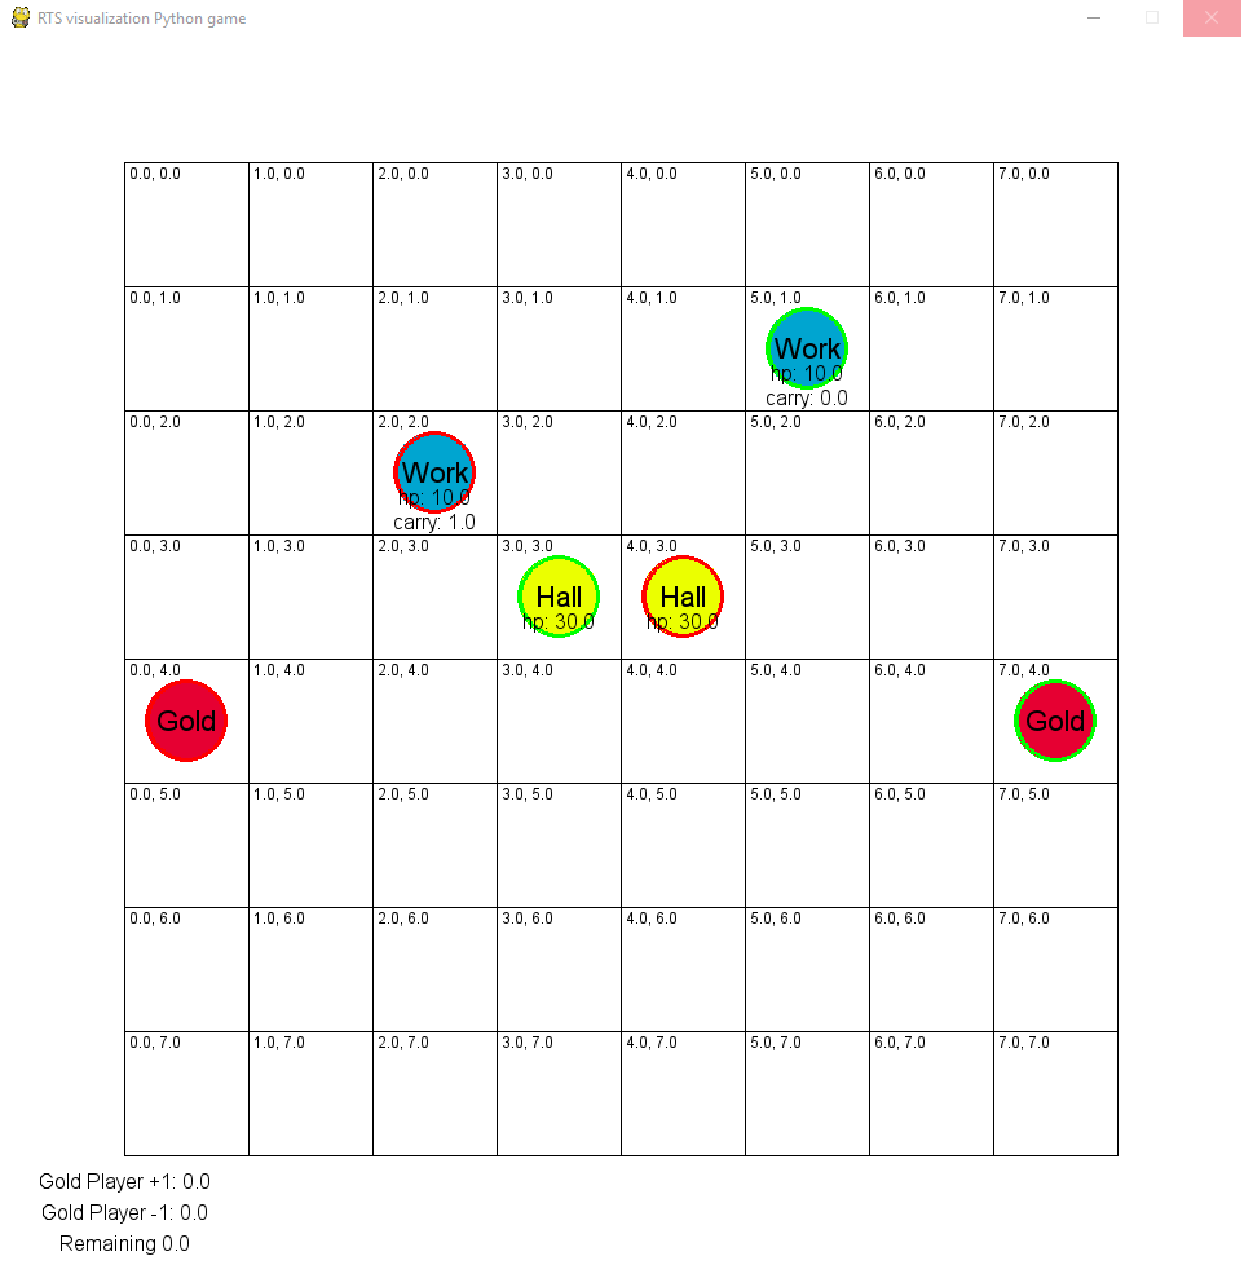
\includegraphics[width=0.9\textwidth]{photos/third-2018-11-14.pdf}
	\end{center}
	\caption{Vizualizacija naučenega modela v Pygame s polji zlata na robovih in glavnimi hišami v sredini. Delavci morajo hoditi daljšo razdaljo do polj zlata, da iz njih naberejo zlatnike, ki jih za tem morajo vrniti v glavno hišo sredi šahovnice. }
	\label{vizualizacijaRezultatovSpremembaZlata}
\end{figure}

Določili smo konfiguracijo igre (Tabela~\ref{tabelLearnConfig}), kjer sta igralca začela s samo glavnima hišama in enim zlatnikom, s katerim sta lahko izgradila po enega začetnega delavca.
Polji zlatnikov sta bili pomaknjeni na rob šahovnice, kar bi zagotavljalo, da morata igralca izbrati mnogo pravih sekvenc pomikanja do polja zlata, pridobiti zlatnike in jih vrniti v glavno hišo, preden bi lahko izgradili novo enoto.

Čeprav se zdi zelo preprosta, ni bila uspešno naučena, saj po skupno 48 urah učenja na Nvidia gtx 1070 grafični kartici in Intel i7 4770 procesorju igralca nista uspešno nabirala zlatnikov in jih vračala v glavno hišo.\\

\begin{table}
	\begin{center}
		\begin{tabular}{p{0.5\linewidth}|p{0.4\linewidth}}
			Tip konfiguracije                          & {\tt Nastavitev parametra} \\ \hline
			{\tt časovna omejitev}                     & 200                     \\
			{\tt iteracije}                            & 30 + 30                 \\
			{\tt epizod}                               & 8                       \\
			{\tt MCTS iskanj}                          & 30                      \\
			{\tt primerjave}                           & 20                      \\
			{\tt zgodovina učnih primerov}             & 8                       \\
			{\tt število epoh}                         & 100                     \\
			{\tt začetni zlatniki}                     & 1                       \\
			{\tt povečevanje zlatnikov}                & 1                       \\
			{\tt zmanjšanje življenjskih točk}         & 20                      \\
			{\tt količina zdravljenja}                 & 20                      \\
			{\tt stroški zdravljenja}                  & 5                       \\
			{\tt število polj}                         & 8 x 8                   \\
			
		\end{tabular}
	\end{center}
	\caption{Nastavitve konfiguracij igre in učnih parametrov pri neuspešnem učenju modela.}
	\label{tabelLearnConfig}
\end{table}

Izdelana delavca sta se prosto sprehajala po šahovnici, kjer sta občasno, vendar naključno, nabrala zlatnike s polja zlatnikov.
Igralca nabranih zlatnikov do izteka časa v skoraj nobeni izmed iger nista vrnila v glavno hišo, kar jima je prinašalo večino neodločenih izidov.
Čeprav sta delavca hodila z nabranimi zlatniki okrog glavne hiše in bi z njihovo vrnitvijo povečala število igralčevih točk, tega nista storila, kar privede do pomislekov o primernosti implementacije MCTS algoritma.
Uteži stanja v raziskovalnem drevesu so bile v tem primeru skoraj naključne, saj se samega učenja ni zgodilo skoraj nič, vendar sam MCTS teh uteži stanj igre ni pravilno popravil.
Za to bi bila možna rešitev nastavitev začetnih stanj igre v nevronski mreži na enaka in ne na naključna, kakor je implementirano v trenutni različici algoritma.

Učenje je potekalo inkrementalno, in sicer 2x po 30 iteracij, pri čemer je igralec po prvi seriji tridesetih iteracij akcije izvajal zelo naključno in so skoraj vse akcije predstavljale naključne premike delavcev po šahovnici.
Po nadaljnjem učenju druge serije sta igralca občasno nabrala zlatnike in jih tudi včasih vrnila v glavno hišo.
To razbitje učenja nam pokaže, da učenje poteka zelo počasi, vendar uspešno.

Tako kot smo opisali v sekciji o poteku učenja~\ref{potekUcenja}, smo v tem primeru naleteli na težavo prekomernega prileganja, saj algoritem ni pravilno prepoznaval neodločenih izidov.
Neodločeni izidi niso bili kaznovani s strani primerjanja dveh modelov, pri katerih so se primerjale samo zmage in porazi novejšega modela proti starejšemu.
Neodločenih izidov je bilo skozi učenje vedno več, pri čemer so pri 40. iteraciji učenja ostali samo neodločeni izidi, z redko zmago katerega izmed modelov.
Rezultat tega je bila naključna hoja delavcev, s čimer so dosegli nov neodločen izid.
Popravek izbire modela je prinašal boljše rezultate, vendar je izbira novejšega modela veliko težja, saj dobra algoritma velikokrat dosežeta neodločen izid, posebej v začetnih stopnjah igre, kjer imata oba igralca malo zlatnikov in figur.

%%%%%%%%%%%%%%%%%%%%%%%%%%%%%%%%%%%%%%%%%%%%%%%%%
Ker je učenje potekalo dokaj neuspešno, smo se odločili zmanjšati velikost šahovnice z 8~x~8 na 6~x~6, kar bi zmanjšalo število možnih stanj igre in poenostavilo nevronsko mrežo, ki bi s to konfiguracijo imela manj končnih uteži, ki se jih mora pravilno naučiti.
Zmanjšali smo tudi število iteracij s 30 na 20, saj bi teoretično bilo potrebnih manj iteracij za učenje manjše šahovnice.

Zmanjševanje šahovnice je privedlo do pričakovanih rezultatov.
Igralca sta občasno nabirala zlatnike, saj je polje zlatnikov v bližini glavne hiše, tako da se delavec postavi med glavno hišo in zlatnike in jih nabira, ne da bi se moral premakniti.
Zaradi nabranih zlatnikov potem igralca izdelata nove delavce in s tem povečata število igralčevih točk.
Število nabranih zlatnikov in izdelanih delavcev je še vedno majhno.
Glavni razlog večjega uspeha te konfiguracije proti prejšnji je bilo postavitev zlatnikov bližje glavni hiši in ne znižanje števila uteži nevronske mreže.

%%%%%%%%%%%%%%%%%%%%%%%%%%%%%%%%%%%%%%%%%%%%%%%%

Poskusili smo še spremembo ustavitvene funkcije na konfiguracijo, ki zmanjšuje število življenjskih točk figuram, kar je opisano v sekciji~\ref{sKillFunction}.

Po določenem številu potez (v našem primeru 90) funkcija prične izmenično zmanjševati življenjske točke igralčevih enot.
Uporaba funkcije v primerjavi z ustavitvenim časom je proizvedla slabše rezultate.
Igralca nabereta manj zlatnikov in posledično izdelata manj figur.

\begin{figure}[h!]
	\begin{center}
		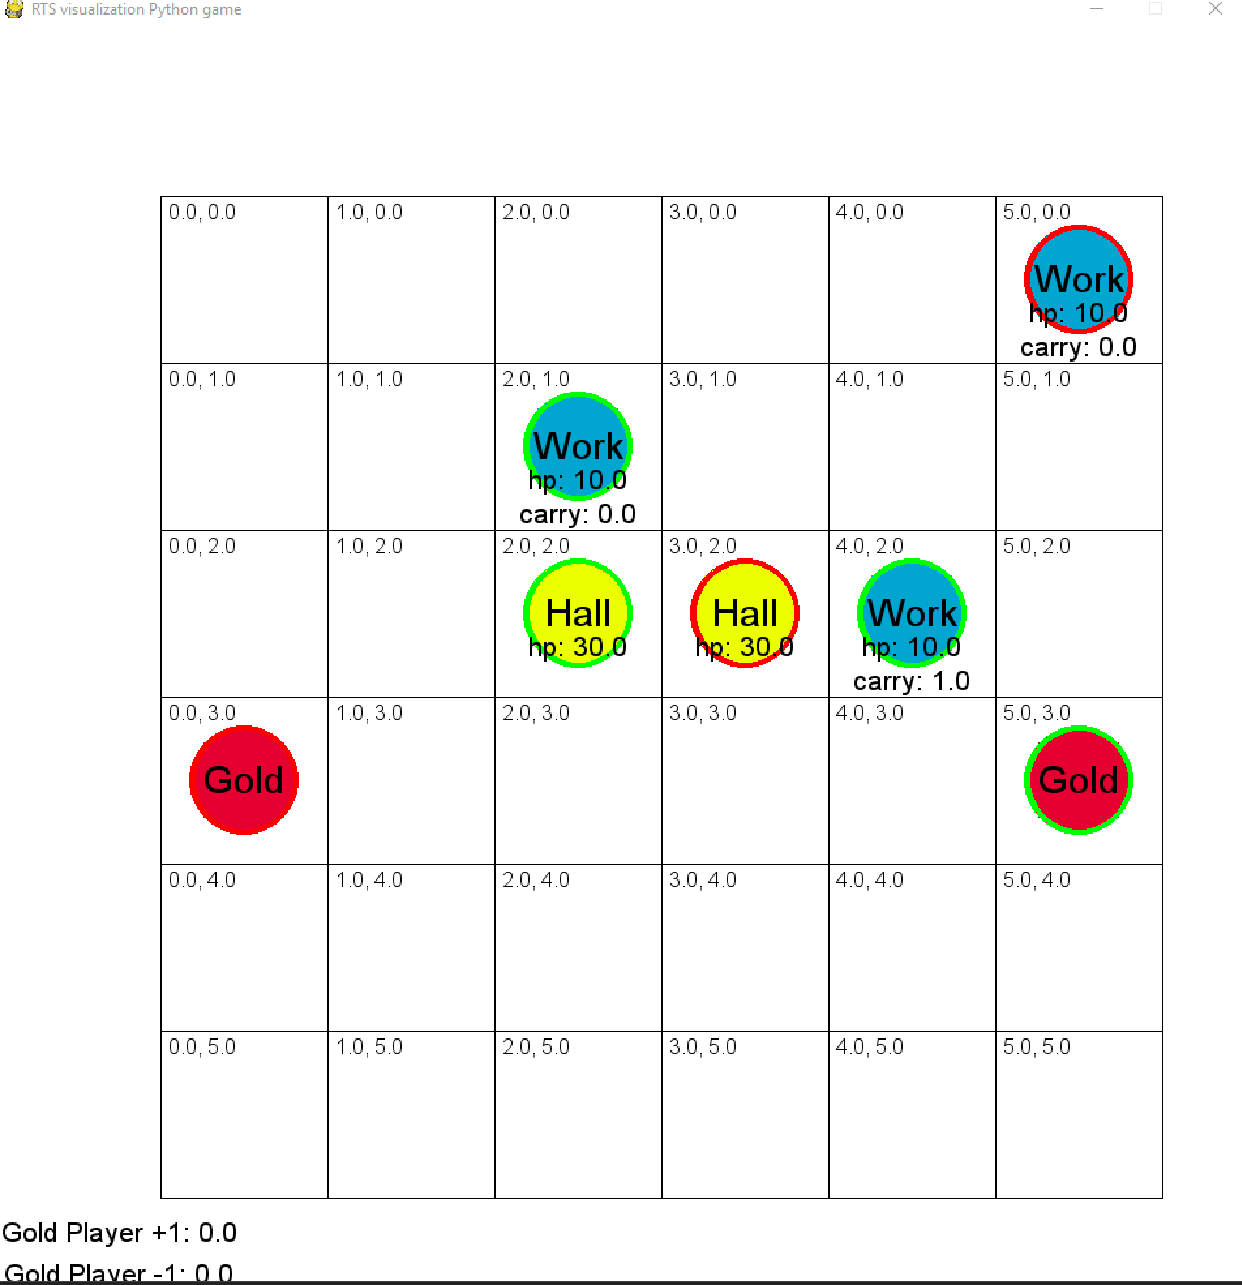
\includegraphics[width=0.6\textwidth]{photos/killFunction.pdf}
	\end{center}
	\caption{Zgornja slika prikazuje stanje igre pri 70. potezi, ki je naučena z uporabo ustavitvene funkcije zmanjšanja življenjskih točk. 
		Igralca sta nabirala zlatnike, in izurila nova delavca, vendar je postopek potekal slabše kakor brez te ustavitvene funkcije. }
	\label{vizualizacijaRezultatovKillFunction}
\end{figure}

Način učenja modela ni primeren, saj ni v skladu z običajnimi RTS igrami, saj se igralčevim enotam življenjske točke ne odštevajo zaradi neznanega razloga.
Možno bi bilo ta način učenja aplicirati v igre, kjer nekatere izmed figur lahko prejmejo znižanje življenjskih točk zaradi naravnih dejavnikov, kot so npr. mraz, strupen plin ipd.

%%%%%%%%%%%%%%%%%%%%%%%%%%%%%%%%%%%%%%%%%%%%%%%%
Sedaj lahko povzamemo zakaj učenje pri zgoraj navedenih konfiguracijah ni potekalo uspešno:
\begin{itemize}
	\item Polji zlatnikov sta bili preveč oddaljeni od glavnih hiš, kar je privedlo do ogromno naključnih premikov, saj igralca nista bila naučena preproste sekvence nabiranja in vračanja zlatnikov, s čimer bi si povečala število točk.
	To je privedlo do veliko neodločenih izidov, iz katerih se igralca nista premaknila, saj primerjava novejšega in starejšega modela ni potekala uspešno.
	\item V konfiguraciji je nastavljeno relativno majhno število iteracij (npr. 60), kjer na koncu vsake iteracije poteka primerjava in učenje ter veliko število epizod (npr. 8), ki generirajo učno množico.
	Zaradi povečane učne množice učenje poteka počasneje kar privede do daljšega časa učenja. Učno množico lahko povečamo tudi na ta način, da ohranimo več iteracij učnih primerov, ki pa je v tem primeru nastavljena samo na 8.	
	\item Najpomembnejši nastavitveni parameter pri učenju je število začetnih zlatnikov.
	Zaradi majhnega števila začetnih zlatnikov (1) sta igralca lahko na začetku igre izdelala samo 1 delavca, s katerim sta zatem morala nabirati in vračati zlatnike.
	Če pa število začetnih zlatnikov povečamo na npr. 10, damo igralcema dovolj veliko število kombinacij začetnih postavitev in izgradnje figur, dokler jima ne zmanjka zlatnikov.
	S tem se naučita pravil, da jima povečevanje števila figur prinaša večje število točk in posledično zmago proti nasprotniku.
	Igralca se zaradi večjega števila kombinacij med sabo na koncu igre tudi večkrat razlikujeta, kar privede do uspešne primerjave novejšega modela proti starejšemu, kjer je manj neodločenih rezultatov.
\end{itemize}

\section{Primerjava kodirnikov}

Določiti moramo še primerni kodirnik, ki bo pospešil učenje in ne bo dajal prednosti določenim poljem šahovnice oziroma igralcem.
Na tej novi konfiguraciji, ki primerja rezultate desetiškega s kodirnikom 1-od-N, smo uporabili vse prejšnje ugotovitve iz neuspešnih učenj.
Za njuno primerjavo smo morali pognati dve identični učenji, z drugačnima kodirnikoma, ki sta vidna v Tabeli~\ref{tableCompareOneHotNumeric}.

\begin{table}
	\begin{center}
		\begin{tabular}{p{0.5\linewidth}|p{0.4\linewidth}}
			Tip konfiguracije                          & {\tt Nastavitev parametra} \\ \hline
			{\tt časovna omejitev}                     & 200                        \\
			{\tt iteracije}                            & 20                         \\
			{\tt epizod}                               & 4                          \\
			{\tt MCTS iskanj}                          & 5                          \\
			{\tt primerjave}                           & 7                          \\
			{\tt zgodovina učnih primerov}             & 5                          \\
			{\tt število epoh}                         & 30                         \\
			{\tt začetni zlatniki}                     & 10                         \\
			{\tt povečevanje zlatnikov}                & 1                          \\
			{\tt zmanjšanje življenjskih točk}         & 20                         \\
			{\tt količina zdravljenja}                 & 20                         \\
			{\tt stroški zdravljenja}                  & 5                          \\
			{\tt število polj}                         & 8 x 8                      \\	
		\end{tabular}
	\end{center}
	\caption{Nastavitve konfiguracij igre in učnih parametrov pri učenjih z 1-od-N in numeričnem kodirnikom.}
	\label{tableCompareOneHotNumeric}
\end{table}

Iz rezultatov, prikazanih z grafoma~\ref{onehot_numeric_score} in~\ref{onehotPrimerjavaAkcij}, je razvidno, da učenje uspešno poteka s kodirnikom 1-od-N tudi pri majhnem številu iteracij (20) z zelo majhnim številom MCTS iskanj in epizod.

Izkazalo se je, da kodiranje 1-od-N prinaša boljše rezultate.
Po ocenitvi modelov z igranjem 100 iger drug proti drugemu je bil rezultat 72~:~15~:~13 (zmaga 1-od-N igralca: zmaga desetiškega igralca: neodločeni izidi).
Zaradi izjemnih rezultatov kodiranja 1-od-N smo ga uporabljali še pri nadaljnjih učenjih.
Za vse akcije smo v Tabeli~\ref{tableencoders} prikazali še razmerja med 1-od-N in desetiškim kodirnikom.

%%%%%%%%%%%%%%%%%%%%%%%%%%%%%%%%%%%%%%%%%%%%%%%%
\begin{table}
	\begin{center}
		\begin{tabular}{p{0.25\linewidth}|p{0.2\linewidth}|p{0.2\linewidth}|p{0.2\linewidth}}
			Akcije             & {\tt Število akcij desetiški kodirnik} & {\tt Število akcij 1-od-N kodirnik} & {\tt razlika v procentih}\\ \hline
			{\tt Premik}       & 49561                   & 43327                      & 12,57\%                                           \\
			{\tt Nabiranje}    & 3026                    & 5638                       & -46,32\%                                          \\
			{\tt Vračanje}     & 2654                    & 5243                       & -49,38\%                                          \\
			{\tt Napad}        & 160                     & 62                         & 61,25\%                                           \\
			{\tt Delavec}      & 2685                    & 3823                       & -29,76\%                                          \\
			{\tt Vojak}        & 666                     & 307                        &53,9\%                                             \\
			{\tt Vojašnica}    & 1052                    & 1215                       & -13,41\%                                          \\
			{\tt Glavna hiša}  & 179                     & 367                        & -51,22\%                                          \\
			{\tt Zdravljenje}  & 9                       & 10                         & -10\%                                             \\
		\end{tabular}
	\end{center}
	\caption{Iz tabele je razvidno da je kodirnik 1-od-N dal večji poudarek na nabiranje zlatnikov in posledično lahko gradil dodatne figure.
	Numerični kodirnik pa je dal večji poudarek na izgradnjo vojaških enot in napadanju.}
	\label{tableencoders}
\end{table}

%%%%%%%%%%%%%%%%%%%%%%%%%%%%%%%%%%%%%%%%%%%%%%%%%%

\begin{figure}[h!]
	\begin{center}
		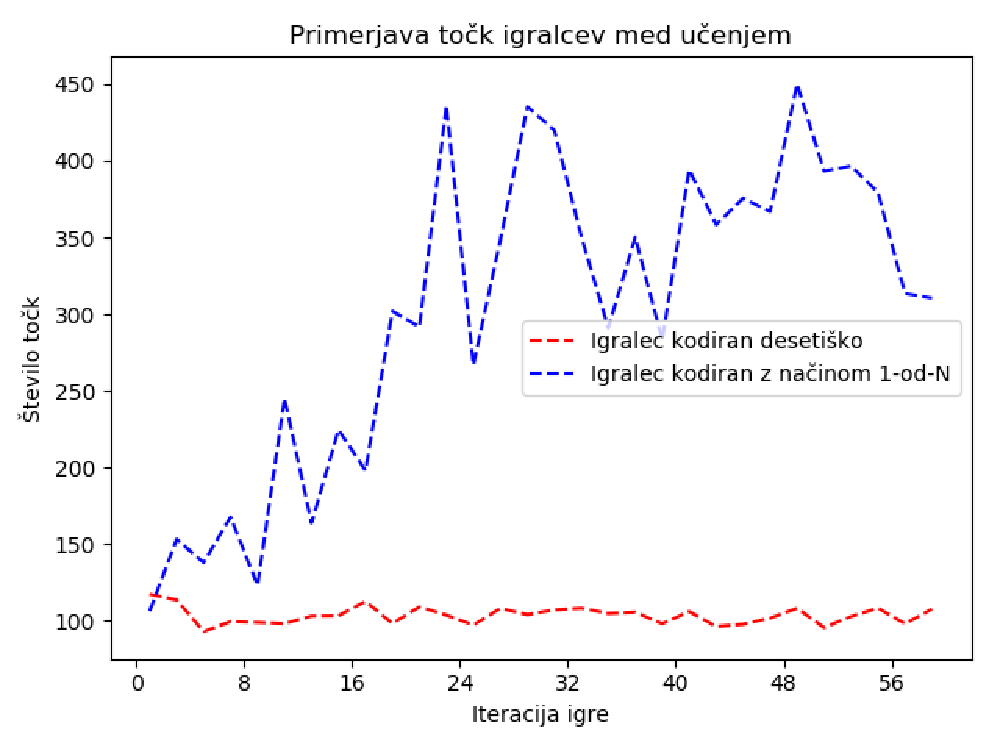
\includegraphics[width=0.8\textwidth]{photos/onehot_numeric_score.pdf}
	\end{center}
	\caption{Graf predstavlja razmerje števila točk z iteracijo igre med učenjem obeh kodirnikov.
		Igralec, kodiran z načinom 1-od-N, je dosegal veliko večje število točk skozi učni postopek, kakor igralec kodiran desetiško, pri katerem učenje ni potekalo uspešno.}
	\label{onehot_numeric_score}
\end{figure}

\begin{figure}[h!]
	\begin{center}
		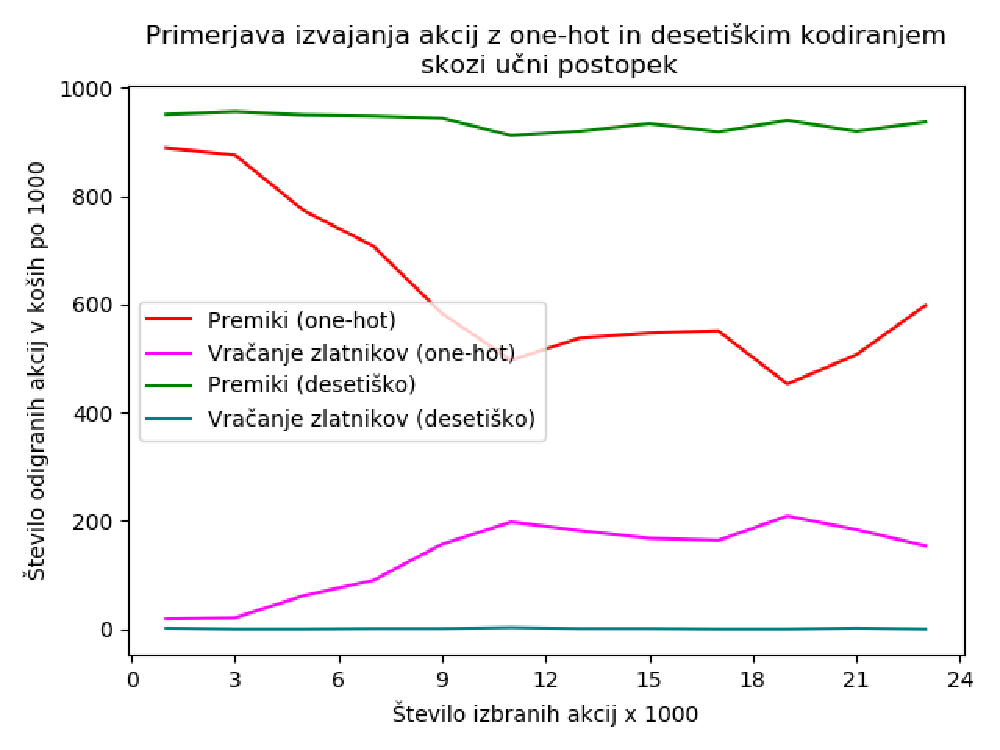
\includegraphics[width=0.8\textwidth]{photos/onehot_numeric_primerjava_akcij.pdf}
	\end{center}
	\caption{Na grafu so prikazane 4 krivulje, ki predstavljajo število posameznih akcij za oba igralca. 
		Prikazane so samo določene akcije, in sicer premiki in vračanje, ostale akcije pa so zaradi preglednosti izpuščene.
		Prikazana je primerjava obeh kodirnikov in njuno izvajanje akcij skozi učni postopek.
		Pri modelu, kodiranem z načinom 1-od-N, je razvidno, da je skozi učni postopek začel zniževati število premikov (rdeča) in hkrati povečeval število vračanj zlatnikov (roza), kar mu je omogočilo večje število točk v ocenjevalni funkciji.
		Igralec je pričel zniževati število premikov, saj so bili na začetku učenja premiki predvsem naključni. Z učenjem pa je igralec dobil idejo, da mu nabiranje zlatnikov prinaša večje število točk.
		Igralec, kodiran desetiško, pa skozi učenje ni izboljšal izbiranja akcij in je še vedno večino akcij posvečal premikanju delavcev in vojaških enot. }
	\label{onehotPrimerjavaAkcij}
\end{figure}

\section{Učenje igranja igre}
S kodirnikom 1-od-N in določenimi pravili igre in učnimi nastavitvami lahko sedaj dokončno naučimo model, da se bo naučil igrati RTS igro.

konfiguraciji, uporabljeni med primerjanjem kodirnikov (Tabela~\ref{tableencoders}), smo spremenili število iteracij in zgodovine učnih primerov, ki sta povečana na 100 in 30.
Pomembno je, da se pri učenju dovoljkrat izvede učenje nevronske mreže in primerjanje trenutnega modela s prejšnjim.
Število ohranjenih iteracij zgodovine učnih primerov je nastavljeno na 30, kar zagotavlja dovolj močno učenje z veliko učnimi primeri, vendar posamezno učenje poteka zelo dolgo, tudi na grafični kartici.

\begin{figure}[h!]
	\begin{center}
		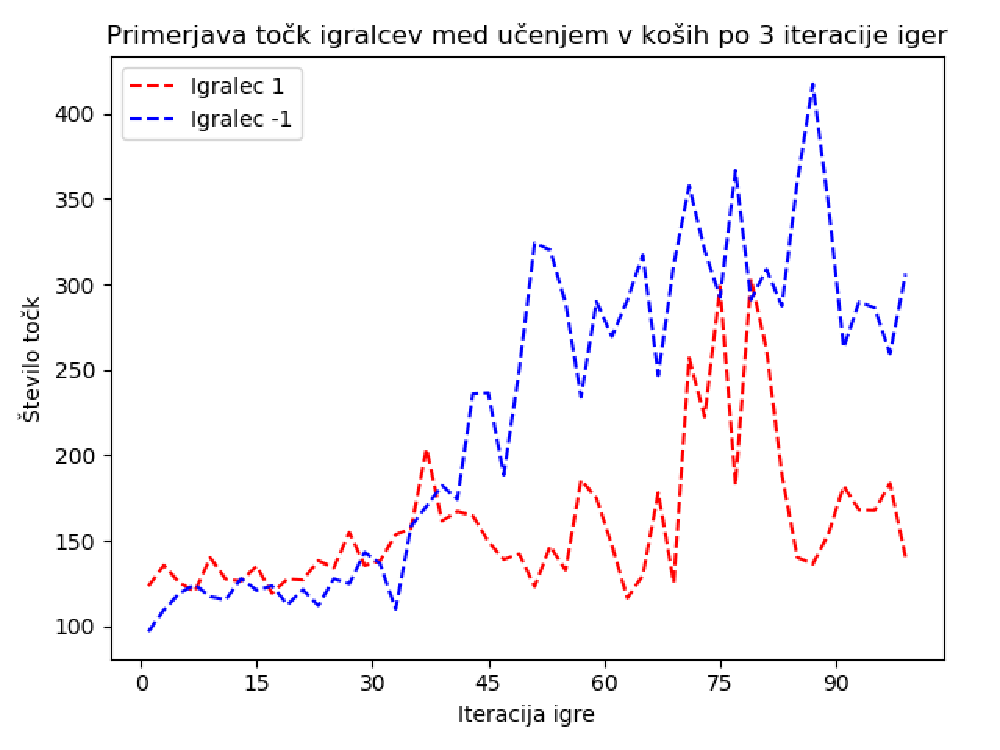
\includegraphics[width=0.8\textwidth]{photos/learn_plot.pdf}
	\end{center}
	\caption{Na grafu je predstavljeno preverjanje trenutnega igralca(-1) proti prejšnjemu igralcu(1) med izvajanjem učnega postopka.
		Razvidno je da je učenje igralca -1 potekalo uspešno, saj se je z iteracijami igre povečevalo število točk.}
	\label{learn_plot}
\end{figure}

\begin{figure}[h!]
	\begin{center}
		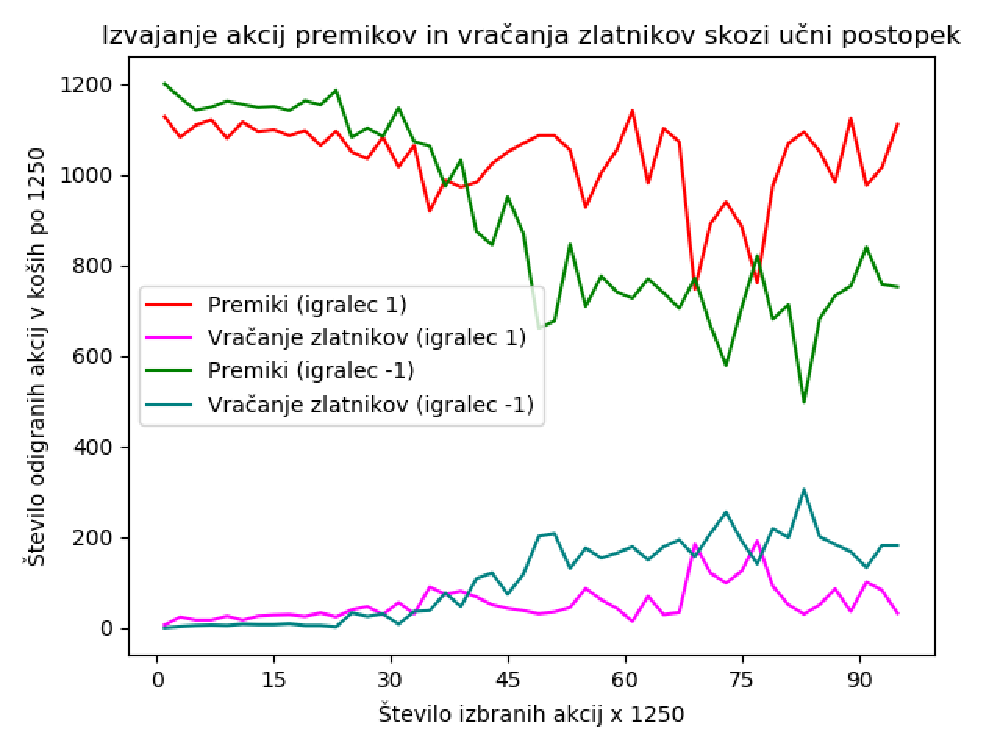
\includegraphics[width=0.8\textwidth]{photos/return_move_learn.pdf}
	\end{center}
	\caption{Tudi tu je kot pri primerjavi akcij kodirnikov (Slika~\ref{onehotPrimerjavaAkcij}) razvidno uspešno učenje s tem da se je zmanjšalo število premikov in povečalo vračanje zlatnikov.
		Posebno se to izkaže pri iteracijah 68 in 76, kjer igralec 1 drastično poveča število vračanj zlatnikov in zmanjša število premikov.}
	\label{return_move_learn}
\end{figure}

\begin{figure}[h!]
	\begin{center}
		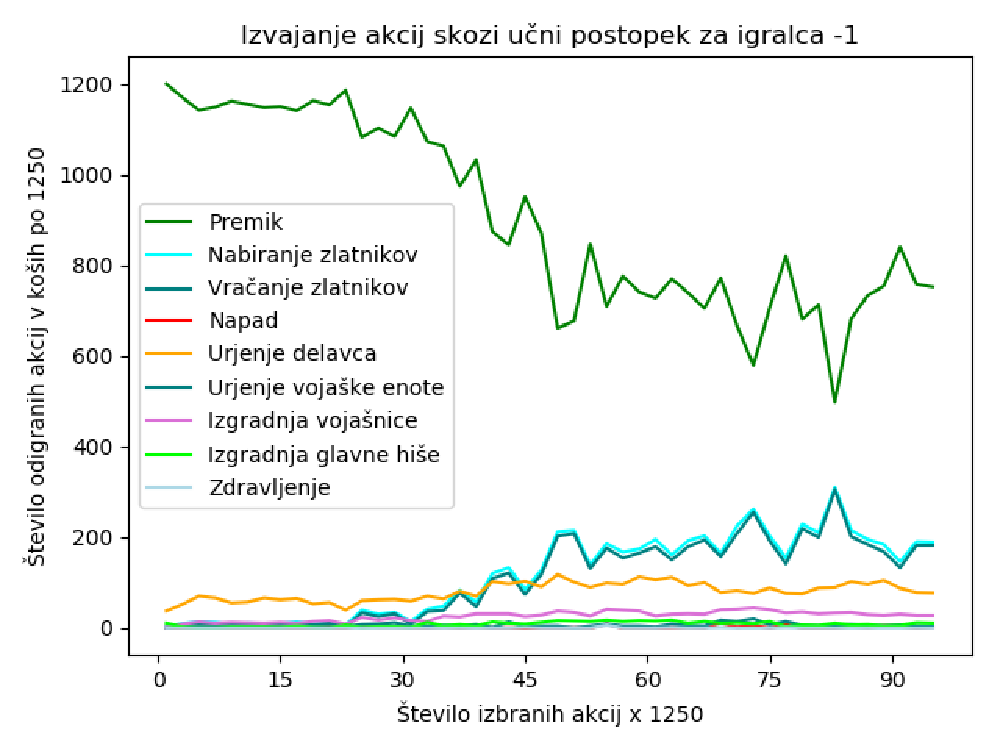
\includegraphics[width=0.8\textwidth]{photos/all_acts_playerminus1.pdf}
	\end{center}
	\caption{Na grafu so predstavljene vse akcije igralca -1 med učnim postopkom.
		Vidno je, da se število premikov zniža, poveča pa se število nabiranj in vračanj zlatnikov, medtem ko število urjenj delavca ostane enako, poveča pa se tudi število izgrajenih vojašnic, kar pa igralcu doprinese več točk kakor urjenje delavca.
		Akcija, kot je npr. napad, ostaja zelo nizko, saj ji igralca ne dajeta prednosti, akcija zdravljenje je pa koristna šele, če je katera od igralčevih enot poškodovana. }
	\label{all_acts_playerminus1}
\end{figure}

S to konfiguracijo se je model uspešno naučil igranja igre~(Slika~\ref{learn_plot}),\\\\tako da zelo pogosto nabira zlatnike in občasno napada nasprotnikove enote (Slika~\ref{all_acts_playerminus1}).
Pri tem učenju je, kakor pri primerjavi kodirnikov, vidna povezava med izvajanjem akcij premikov in vračanjem zlatnikov, ki največ vpliva na izboljšavo točk~(Slika~\ref{return_move_learn}).
Igralca napadata nasprotnikove enote, ko so postavljene poleg vojaške enote, vendar se taktično lovljenje nasprotnikovih figur z vojaškimi enotami ne zgodi.
Igralca pa še vedno ne zaključita igre z eliminacijo nasprotnika, saj to ni njuna glavna prioriteta, ker sta bolj osredotočena na povečevanje svojih točk in ne na znižanje nasprotnikovih z napadanjem.
To privede v šahovnico, ki ima veliko polj zasedenih z novimi figurami~(Slika~\ref{pit_100_game1}).

\begin{figure}[h!]
	\begin{center}
		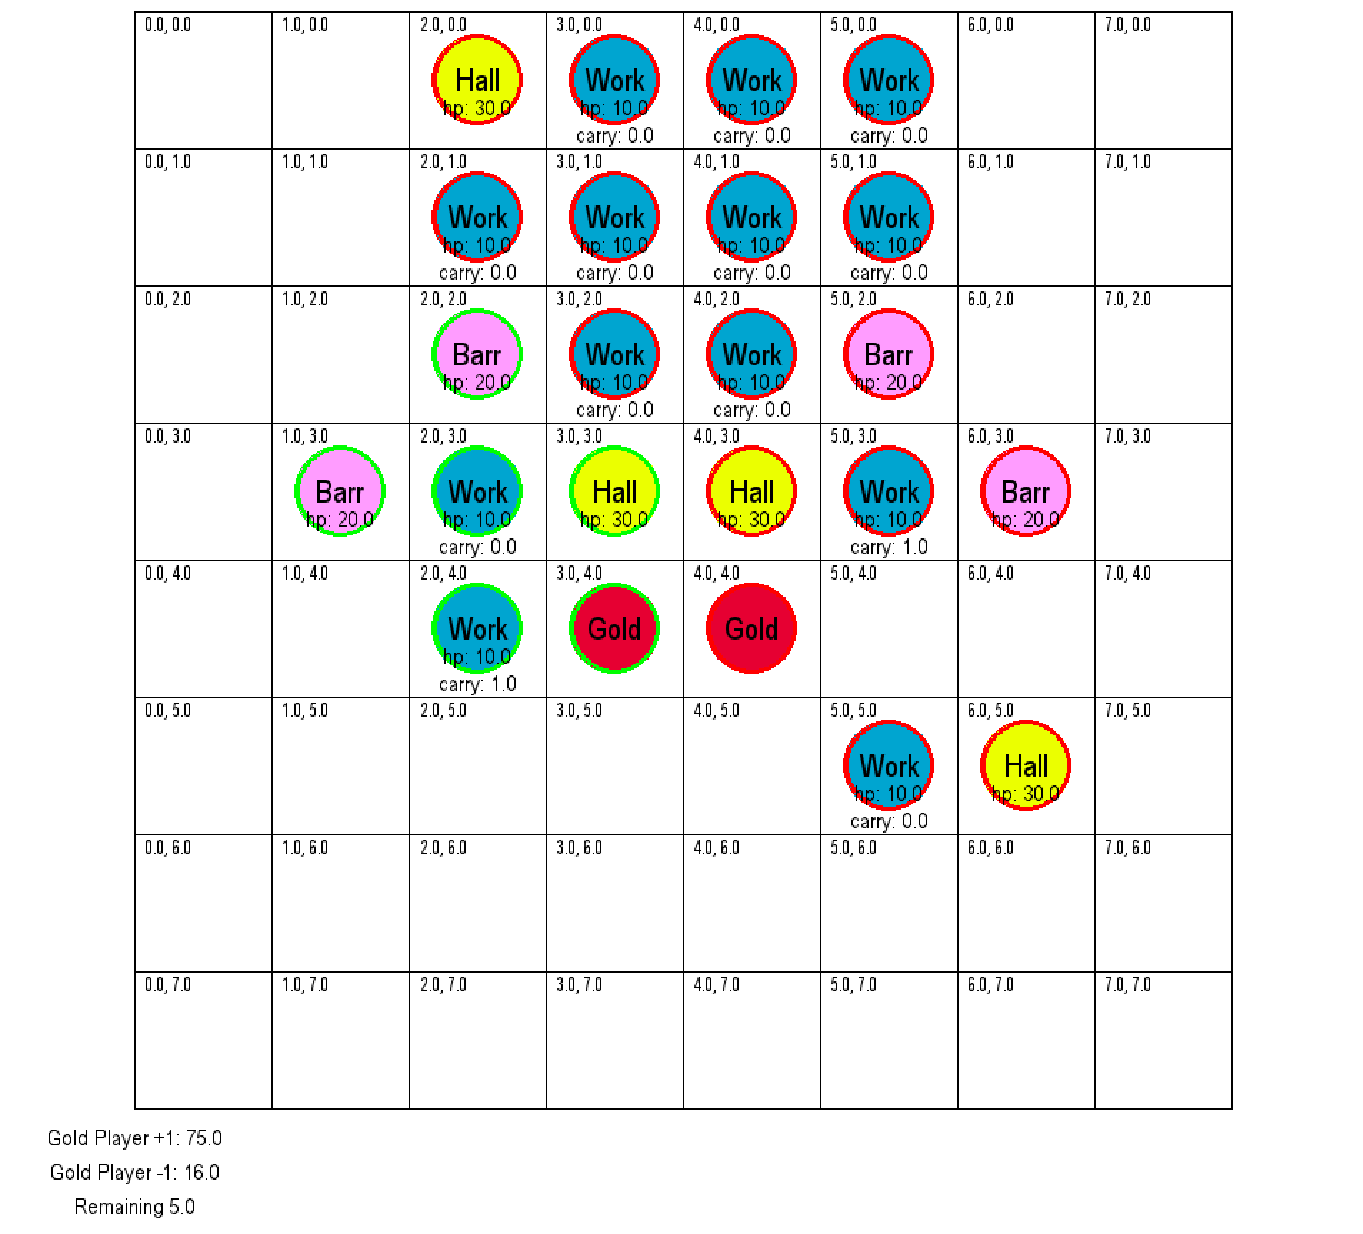
\includegraphics[width=0.8\textwidth]{photos/pit_100_game1.pdf}
	\end{center}
	\caption{Primerjanje naučenega modela v Pygame. 
		Vidno je, da sta igralca izdelala veliko število figur in redno nabirala zlatnike. 
		V levem spodnjem kotu je razvidno, koliko zlatnikov ki jih lahko zapravita za urjenje enot in gradnjo infrastrukture imata igralca v banki.
		Igralec 1 (zelena) ima ogromno število zlatnikov, ki mu doprinašajo dodatne točke z ocenjevalno funkcijo.
		Vsak izmed igralcev ima vsako igro na voljo 100 potez, pri katerih porabi 2 potezi za nabiranje in vračanje zlatnikov, če je delavec postavljen zraven polja zlatnikov in glavne hiše, na kar po posameznem vračilu igralec pridobi 3 zlatnike. Največje možno število zlatnikov za igralca je tako 147, saj mora igralec prvo potezo izgraditi delavca, z ostalimi pa lahko nabere po 3 zlatnike vsako drugo potezo.
		Igralec je pridobil 75 zlatnikov, s tem da je izdelal še dodatnega delavca (1 zlatnik in 1 poteza) in dve vojašnici (8 zlatnikov in 2 potezi).
		Igralec je tako veliko število potez porabil za nabiranje in vračanje zlatnikov.
		Medtem ko se je igralec -1 (rdeča) bolj osredotočil na urjenje delavcev in izgradnjo dodatnih glavnih hiš, ki mu doprinesejo veliko število točk, ampak ima zato manj zlatnikov v banki.}
	\label{pit_100_game1}
\end{figure}

\begin{figure}[h!]
	\begin{center}
		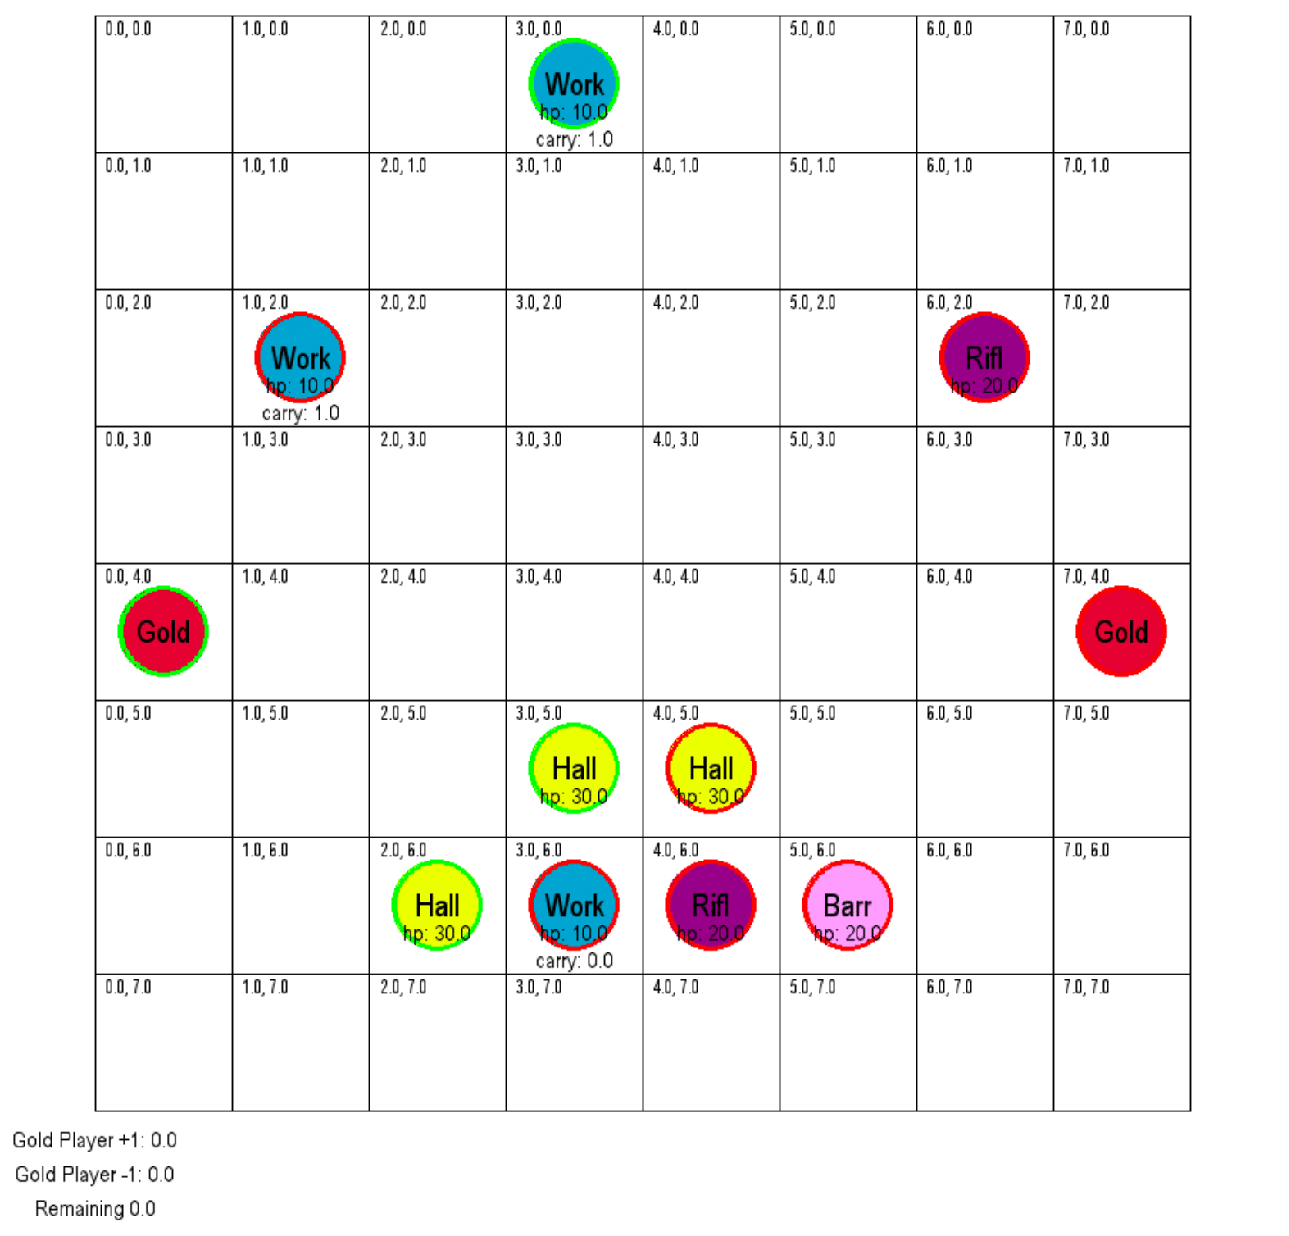
\includegraphics[width=0.8\textwidth]{photos/pit_minerals_apart_100.pdf}
	\end{center}
	\caption{Primerjava naučenega modela z drugačno postavitvijo šahovnice, pri katerih sta polji zlatnikov na robovih.
		Igralca uspešno nabereta zlatnike, ko se približata polju zlata, in jih vrneta, ko se približata glavni hiši.
		Napadi vojaških enot so pri tej konfiguraciji bolj očitni, saj ni velikega števila delavcev in drugih figur kot v prejšnem primeru (Slika~\ref{all_acts_playerminus1}).}
	\label{pit_minerals_apart_100}
\end{figure}

Igralec, naučen s to konfiguracijo, tudi prepozna polja zlatnikov na oddaljenem polju na šahovnici brez posebnega učenja (Slika~\ref{pit_minerals_apart_100}).
Te zlatnike igralec pobere in jih vrne v glavno hišo, ko delavec pride zraven nje, vendar igralec ne izvaja namernih premikov delavca do polja zlatnikov, da bi jih nabral in vrnil v glavno hišo.
Z naknadno konfiguracijo, kjer so polja zlatnikov na robovih šahovnice, igralec ne pridobi tako dobrih rezultatov, saj nevronska mreža ni naučena na pozicijsko neodvisnost.
%To bi bilo možno popraviti, tako da bi vsako iteracijo igre spremenil začetno konfiguracijo pozicij glavnih hiš in polj zlata na šahovnici.

%%%%%%%%%%%%%%%%%%%%%%%%%%%%%%%%%%%%%%%%%%%%%%%%

\section{Vizualizacija rezultatov v pogonu Unreal Engine}
Rezultate smo vizualizirali v pogonu Unreal Engine 4, ki ga je izdelalo podjetje Epic Games.
Izbiranje potez deluje izmenjujoče z zamikom pol sekunde, da se akcije končajo, preden se pošlje nov zahtevek z novim kodiranjem stanja igre.
Če so v UE4 nastavljena enaka pravila, kot na primer stroški enot in število začetnih zlatnikov, kot v Python skripti, potem igralca igrata igro identično kot v Pygame.

\begin{figure}[h!]
	\begin{center}
		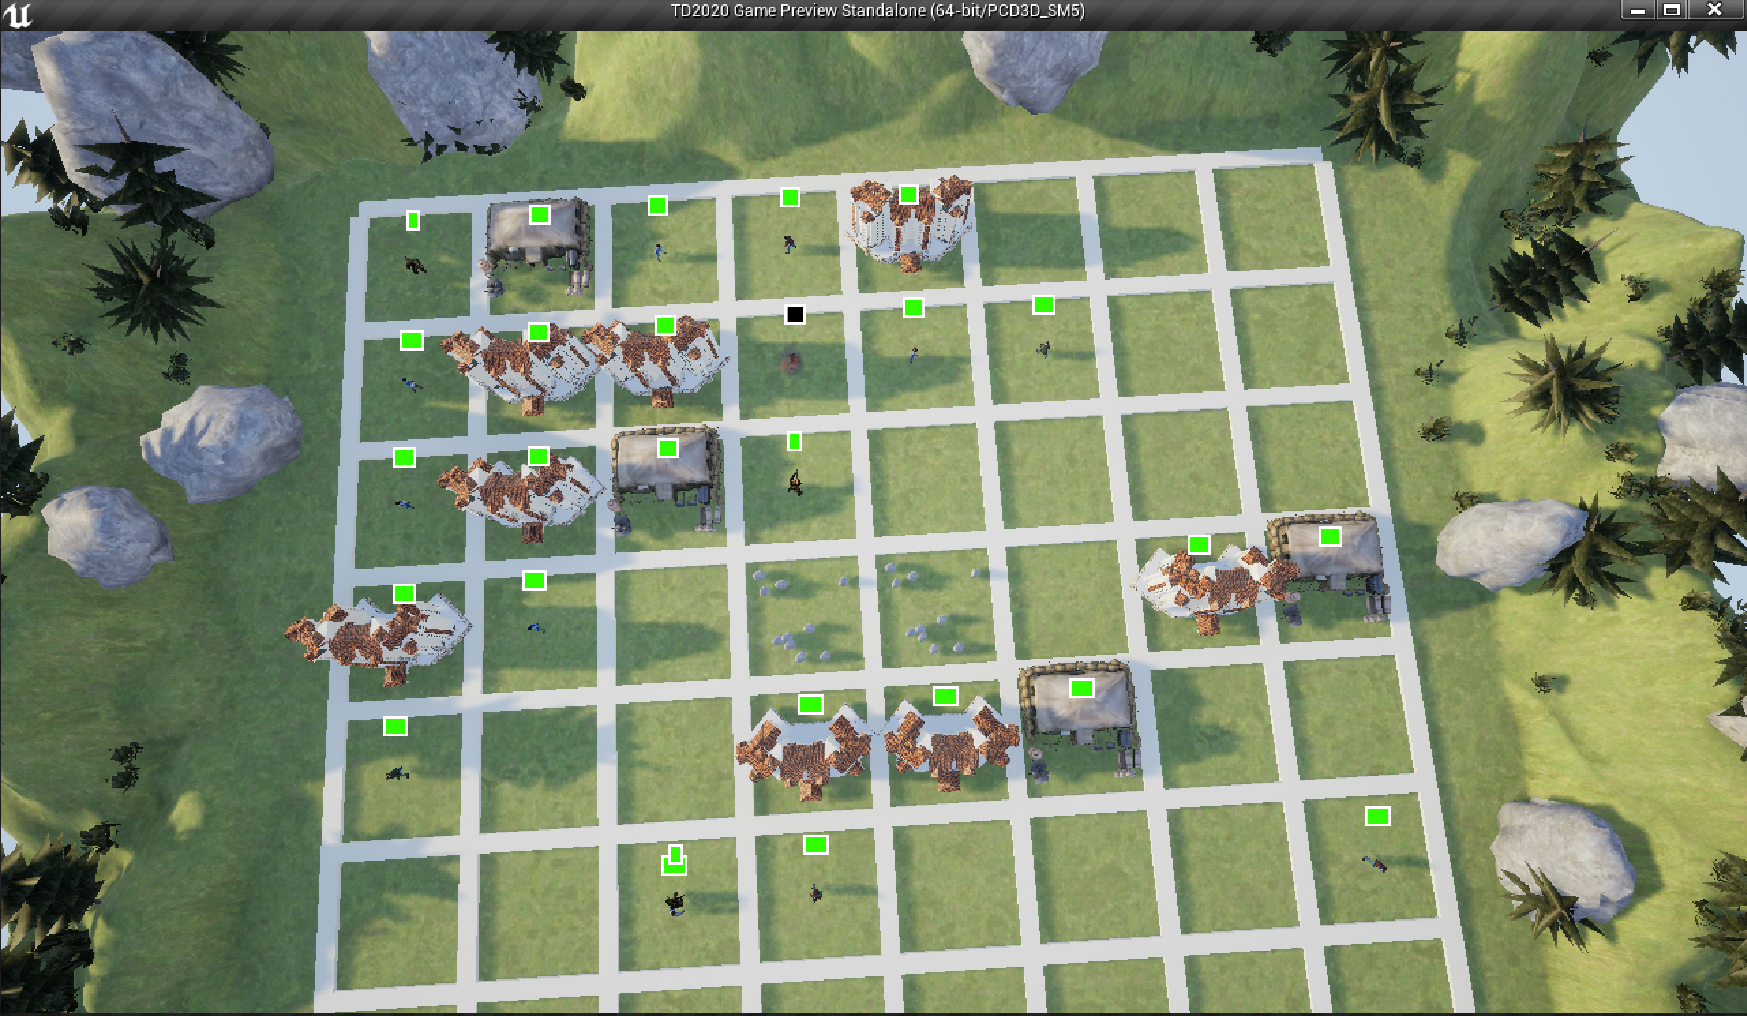
\includegraphics[width=0.8\textwidth]{photos/ue4attack.pdf}
	\end{center}
	\caption{Igranje dveh računalniških nasprotnikov enega proti drugemu v UE4. 
		V sredini vidimo glavni hiši in polja zlata, okrog pa vojašnice, delavce, glavne hiše in vojaške enote.
		Na sliki je vidnen napad vojaške enote na enega izmed delavcev. }
	\label{visualization_ue4}
\end{figure}

Igranje proti računalniškemu nasprotniku je z uporabo tega algoritma možno, vendar računalniški nasprotnik ne igra dovolj inteligentno, da bi bil primeren za njegovo aplikacijo v modernejše strateške igre, kjer bi ga lahko implementirali kot glavnega računalniškega nasprotnika.
Naučen model bi bil primeren samo za določen zemljevid, če ga seveda ne bi učili na različnih postavitvah šahovnice, kjer bi dodajali zasedena polja ipd.

%%%%%%%%%%%%%%%%%%%%%%%%%%%%%%%%%%%%%%%%%%%%%%%%%%%%%%%%%%%%%%%%%%%%%%%%%%%%%%%%%%%%%%%%%%%%%%%%%%%%%%%%%%%%%%%%%%%%%%%%
%%%%%%%%%%%%%%%%%%%%%%%%%%%%%%%%%%%%%%%%%%%%%%%%%%%%%%%%%%%%%%%%%%%%%%%%%%%%%%%%%%%%%%%%%%%%%%%%%%%%%%%%%%%%%%%%%%%%%%%%
%%%%%%%%%%%%%%%%%%%%%%%%%%%%%%%%%%%%%%%%%%%%%%%%%%%%%%%%%%%%%%%%%%%%%%%%%%%%%%%%%%%%%%%%%%%%%%%%%%%%%%%%%%%%%%%%%%%%%%%%
%%%%%%%%%%%%%%%%%%%%%%%%%%%%%%%%%%%%%%%%%%%%%%%%%%%%%%%%%%%%%%%%%%%%%%%%%%%%%%%%%%%%%%%%%%%%%%%%%%%%%%%%%%%%%%%%%%%%%%%%
%%%%%%%%%%%%%%%%%%%%%%%%%%%%%%%%%%%%%%%%%%%%%%%%%%%%%%%%%%%%%%%%%%%%%%%%%%%%%%%%%%%%%%%%%%%%%%%%%%%%%%%%%%%%%%%%%%%%%%%%

\chapter{Diskusija}
\label{chdiskusija}

Kot smo ugotovili v poglavju~\ref{chrezultati}, učenje modela poteka počasi, vendar se uspešno uči.
Zasnova opisa igre in njenega kodiranja je prava, ker učenje poteka uspešno.
Počasi poteka zaradi ustavitvenega pogoja in ocenjevalnih funkcij, ki ugotovjo zmagovalca ob ustavitvenem pogoju, čeprav mogoče ni pravi zmagovalec ob koncu igre.
MCTS naredi zelo majhno število iskanj in ne simulira igre do konca oziroma do določene globine, kjer bi ugotovil stanje igre ter to stanje propagiral nazaj po drevesu.
Stanje igre pridobi od naučenega modela, ki na začetku učenja ni pravo.
Možna izboljšava bi bila uporaba MCTS s simulacijo igre do ustavitvenega pogoja v začetku učenja namesto napovedi nevronske mreže, saj te niso prave.

Pri opisu igre je veliko problemov povzročalo uravnovešanje parametrov igre, kot je na primer število vrnjenih zlatnikov, količina in cena zdravljenja ipd.
Dober primer neuravnovešene konfiguracije igre sta bila prav količina in cena zdravljenja.
Pri napačni konfiguraciji je igralec stalno samo nabiral zlatnike in zdravil svoje figure, tako da je dosegal vedno večje število narejenih potez pri ustavitvenem pogoju z zmanjševanjem števila življenjskih točk.
Zaradi tega je učenje potekalo zelo počasi, saj so posamezne igre trajale predolgo, preden so se zaključile.
Podoben primer nastavitve parametrov je število začetnih zlatnikov, ki zelo vpliva na hitrost učenja modela, s tem da igralcema poda dovolj veliko število možnih kombinacij gradnje stavb in urjenja figur, da rezultat po časovnem izteku ni neodločen.

Največ problemov je pri opisu igre povzročal ustavitveni pogoj.
Časovna omejitev na npr. 200 potez se ne preslika naravno v moderno 3D-računalniško igro, saj te običajno nimajo časovne omejitve.
Prav tako ni običajno zniževa- nje življenjskih točk igralčevih enot po določenem času, razen če je scenarij igre postavljen v nevarno okolico.
Ocenitev stanja igre po časovni omejitvi ni najboljša, saj je pridobljena po preprosti formuli, ki seveda ne zajame vseh dejavnikov igre.

Algoritem se da dobro aplicirati v pogon Unreal Engine z nekaj vtičniki, opisanimi v razdelku~\ref{UnrealEngine}. Več igralcev lahko na istem računalniku zahteva priporočila akcij. 
Če igra poteka preko mreže, vsak igralec na svojem računalniku poganja algoritem, ki ne ovira delovanja drugih TensorFlow sej na računalnikih drugih igralcev.
%Sama igra, napisana v programskem jeziku Python, na kateri je bil naučen model, se ne preslika direktno v dejansko igro, napisano v Unreal Engine.

V tej igri se akcije ne zgodijo takoj ob izvršitvi ukaza, saj vojaške enote in delavci potrebujejo nekaj časa, da se premaknejo na drugo lokacijo, izvedejo akcijo, kot na primer nabiranje zlatnikov, ki se tudi ne izvede takoj.
Zaradi trajanja akcij, asinhronosti pridobivanja priporočila, ki jih vrača Python modul, se lahko zgodi, da stanje igre ni več takšno, kakršno je bilo pri pošiljanju zahtevka za priporočilo, in bi bila priporočena akcija z asinhrono skripto drugačna. 
V nekaterih primerih se ob takih pogojih dve figuri premakneta na isto polje, oziroma se izgradi stavba na polju, kjer je trenutno enota. 
Rešitev za to je vpeljava zahtevanja priporočil akcij, ko so te zaključene, ter nezmožnost izvajanja akcij v času od zahtevka priporočila do vrnjenega rezultata.
Ta rešitev je primerna za strateške igre, vendar ne za podkategorijo realno-časovnih strateških iger, ki pa zahtevajo takojšno napoved akcije.

Naučeni model vrača samo 1 akcijo, ki ne more vključevati večje skupine figur, kot na primer vseh vojaških enot, da se premaknejo proti nasprotniku za napad.
Večina teh akcij, kot na primer pomik gor, dol, napad gor ipd., je tudi omejenih na sosednja polja, kar tudi ni primerna aplikacija v dejansko igro, kjer se lahko figure premikajo po poljubnih dovoljenih točkah in smereh.

%%%%%%%%%%%%%%%%%%%%%%%%%%%%%%%%%%%%%%%%%%%%%%%%%%%%%%%%%%%%%%%%%%%%%%%%%%%%%%%%%%%%%%%%%%%%%%%%%%%%%%%%%%%%%%%%%%%%%%%%
%%%%%%%%%%%%%%%%%%%%%%%%%%%%%%%%%%%%%%%%%%%%%%%%%%%%%%%%%%%%%%%%%%%%%%%%%%%%%%%%%%%%%%%%%%%%%%%%%%%%%%%%%%%%%%%%%%%%%%%%
%%%%%%%%%%%%%%%%%%%%%%%%%%%%%%%%%%%%%%%%%%%%%%%%%%%%%%%%%%%%%%%%%%%%%%%%%%%%%%%%%%%%%%%%%%%%%%%%%%%%%%%%%%%%%%%%%%%%%%%%
%%%%%%%%%%%%%%%%%%%%%%%%%%%%%%%%%%%%%%%%%%%%%%%%%%%%%%%%%%%%%%%%%%%%%%%%%%%%%%%%%%%%%%%%%%%%%%%%%%%%%%%%%%%%%%%%%%%%%%%%
%%%%%%%%%%%%%%%%%%%%%%%%%%%%%%%%%%%%%%%%%%%%%%%%%%%%%%%%%%%%%%%%%%%%%%%%%%%%%%%%%%%%%%%%%%%%%%%%%%%%%%%%%%%%%%%%%%%%%%%%

\chapter{Zaključek}
\label{chzakljucek}
V diplomski nalogi smo povzeli, kaj realno-časovna strateška igra.
Pregledali smo nivoje nadzorovanja figur in abstrakcije prostora ter s kakšnega zornega kota nanje gledajo nevronske mreže.
Za tem smo se podali v raziskovanje algoritmov za učenje te strateške igre in naleteli na algoritem AlphaZero.
Na hitro smo pregledali njegovo zgodovino in korake k samostojnemu algoritmu, ki je primeren za reševanje poljubne igre z metodami samoučenja.
Ta algoritem smo potem podrobneje pregledali, da smo njegov proces učenja in igranja iger razumeli in opisali svojo strateško igro v jeziku Python.

Določili smo pravila igre in glavne cilje, ki jih strateška igra mora imeti.
Pri tem smo morali paziti, da smo se držali okvira Surag-Nairjeve implementacije algoritma AlphaZero~\cite{alphazerogeneral}, da smo lahko zanj pripravili svojo strateško igro, ki je združljiva z njegovim algoritmom.
Nato smo določili akcije, ki jih figure lahko izvajajo, in jih abstrahirali, tako da so za algoritem nedvoumne in hitre.
Da smo nevronski mreži lahko podali stanje igre, smo ga morali pravilno zakodirati.
Izbrali smo desetiški in 1-od-N način kodiranja, med katerima se je 1-od-N izkazal kot uspešnejši, saj v prednost ne postavlja večjih zakodiranih števil kot boljših.
Nato smo ugotovili pravi način evalvacije stanja igre in njen ustavitveni pogoj.

Določili smo ustavitveno oslabitveno funkcijo, ki dovoljuje bolj aktivnim igralcem daljše igranje, vendar jih kaznuje iz razlogov, ki sami strateški igri niso naravni.
Drugi pristop ustavitvenega pogoja je bil časovni iztek, pri katerem se je po določenem številu potez presodilo, kateri igralec je zmagovalen po določenem kriteriju.
Ko smo imeli opisano igro, smo morali ugotoviti primerne nastavitve in jih uporabiti pri samem učenju igre in izbrati parametre.

Potem smo pripravili vizualizacijo igre v jeziku Python z modulom Pyga- me, ki prikaže igro v preprosti šahovnici in figure s krogci.
V pogonu Unreal Engine 4 smo pripravili bolj kompleksno strateško igro, ki je boljša predstavitev dejanske realno-časovne strateške igre.
V tej igri pošiljamo zahtevke za akcije preko vtičnika v Python skripto, v katero podamo trenutno stanje igre in nazaj dobimo priporočeno akcijo.
Zahtevke lahko pošilja računalniški nasprotnik ali človeški igralec, ko v najboljšo akcijo ni prepričan.
Nato smo se posvetili predvsem učenju modelov z različnimi konfiguracijami ter jih vizualizirali v Pygame in Unreal Engine.

Ugotovili smo, da je učenje počasnejše zaradi kompleksnosti igre in načina zgradbe nevronske mreže, vendar poteka uspešno, s tem da zaradi izbire kodirnika 1-od-N ne daje večje prednosti igralcu 1 kot -1.
Model smo uspešno naučili osnovnega igranja igre, s tem da je igralec nabiral zlatnike, ustvarjal nove figure in občasno napadal nasprotnikove enote.

Diplomska naloga je v času pisanja (januar 2019) zelo aktualna, saj je ekipa podjetja DeepMind razvila algoritem AlphaStar, ki je premagal dva profesionalna StarCraft 2 igralca ekipe Team Liquid, in sicer TLO in MaNa~\cite{alphastar}.
Poleg spodbujevalnega učenja, opisanega v diplomski nalogi, je AlphaStar uporabljal še sistem lig, ki so pomagale agentom razviti različne vrste taktik in strategij~(Slika~\ref{photo_alphastar}).
Zaradi popularnosti igre StarCraft 2 znotraj žanra realno-časovnih strateških iger, obstaja tudi veliko število posnetkov iger, iz katerih se je AlphaStar naučil ob začetku učenja.
Na tem osnovnem znanju pa se je začel učiti s pomočjo spodbujevalnega učenja.
Igranje realno-časovnih strateških iger je zelo aktualno na področju raziskovanja umetne inteligence, ki pa se hitro razvija.\\\\
\begin{figure}[h!]
	\begin{center}
		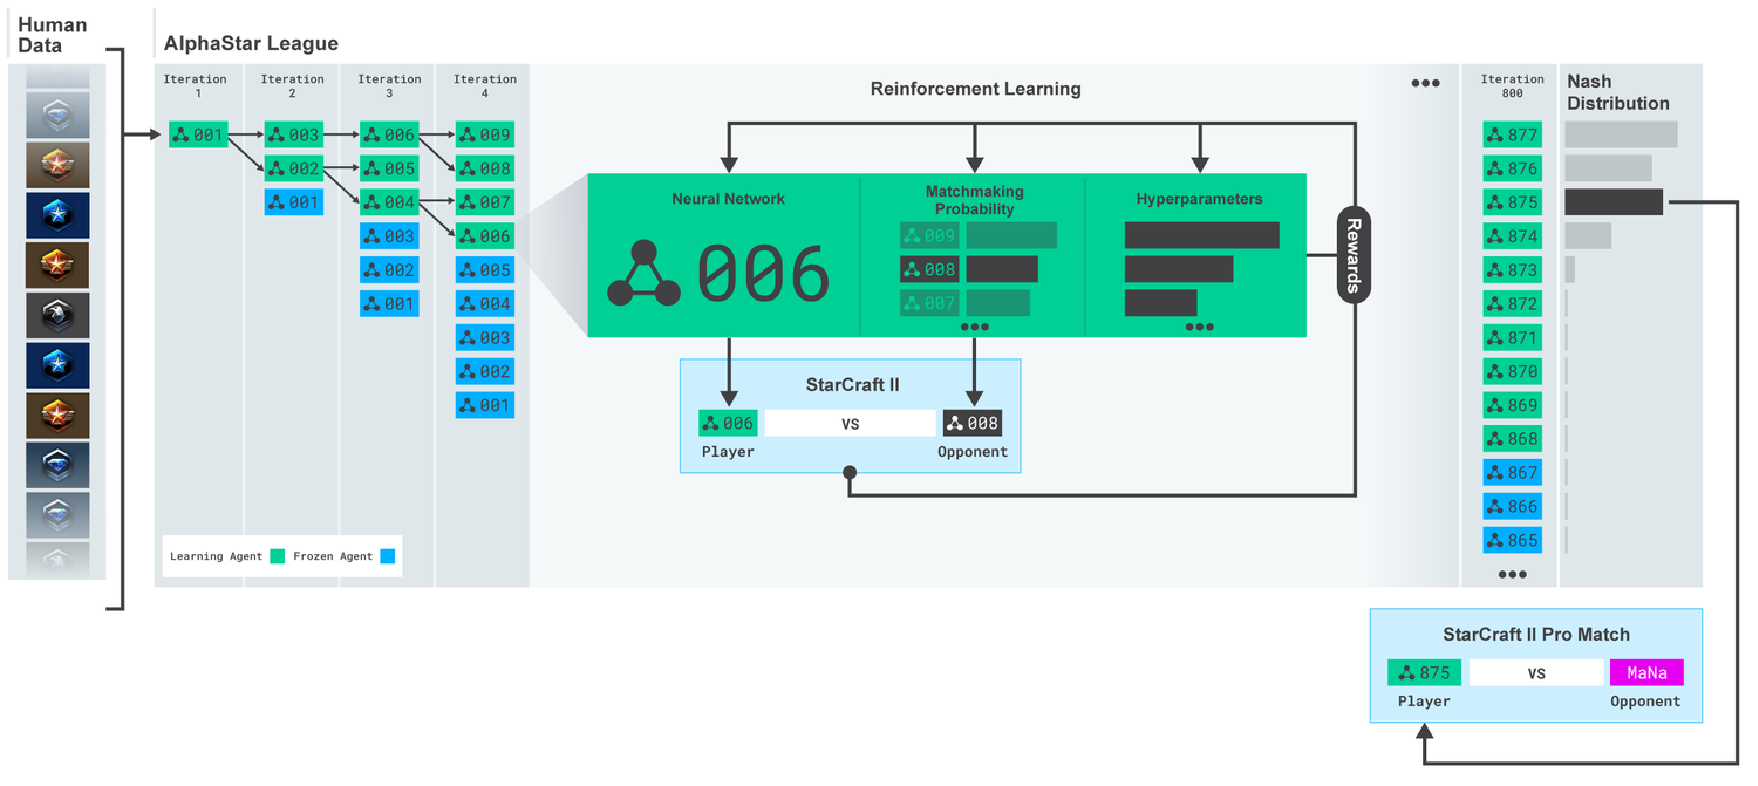
\includegraphics[width=1\textwidth]{photos/alphastar.pdf}
	\end{center}
	\caption{Sistem lig, uporabljen v algoritmu AlphaStar. }
	\label{photo_alphastar}
\end{figure}

Diplomska naloga je dober prispevek k Surag-Nairjevim igram za AlphaZero, ki razširi preproste igre črno-belih figur v figure večih atributov.
V to igro smo pripeljali tudi časovne kompleksnosti in jo razširili z vizualizacijo v Pygame in Unreal Engine 4.
Igro, izdelano v UE4~\cite{td2020}, in AlphaZero General algoritem s Pygame igro~\cite{pygameAlphaZeroGeneral} in njenimi izdajami smo dodali na spletno gostovanje GitHub pod odprto licenco.

\newpage %dodaj po potrebi, da bo številka strani za Literaturo v Kazalu pravilna!
\ \\
\clearpage
\addcontentsline{toc}{chapter}{Literatura}
\bibliographystyle{plain}
\bibliography{literatura}


\end{document}

